%% LyX 2.1.4 created this file.  For more info, see http://www.lyx.org/.
%% Do not edit unless you really know what you are doing.
\documentclass[a4paper,oneside,brazil,11pt,a4paper,openright,titlepage,usenames,dvipsnames]{book}
\usepackage[T1]{fontenc}
\usepackage[utf8]{inputenc}
\setcounter{secnumdepth}{3}
\setcounter{tocdepth}{3}
\usepackage{array}
\usepackage{verbatim}
\usepackage{calc}
\usepackage{textcomp}
\usepackage{amssymb}
\usepackage{graphicx}
%\usepackage[mathscr]{euscript}
\usepackage{eucal}



%Pacote para uso de pseudo código
\usepackage{algorithm}
\usepackage{algorithmicx}
\usepackage{algpseudocode}

%Mudando para o pt-br
\makeatletter
\renewcommand{\ALG@name}{Algoritmo}
\makeatother

%lista de símbolos
\usepackage{nomencl}
\usepackage{listings}
\renewcommand{\nomname}{Lista de Símbolos}
\makenomenclature
\newcommand\T{\rule{0pt}{2.6ex}}
\newcommand\B{\rule[-1.2ex]{0pt}{0pt}}

%letras estilizadas \mathpzc \mathantt
\DeclareMathAlphabet{\mathantt}{OT1}{antt}{li}{it}
\DeclareMathAlphabet{\mathpzc}{OT1}{pzc}{m}{it}

\makeatletter

%%%%%%%%%%%%%%%%%%%%%%%%%%%%%% LyX specific LaTeX commands.
\pdfpageheight\paperheight
\pdfpagewidth\paperwidth

%% Because html converters don't know tabularnewline
\providecommand{\tabularnewline}{\\}

%%%%%%%%%%%%%%%%%%%%%%%%%%%%%% User specified LaTeX commands.
% Classe alternativa, apropriada para impressão frente-verso. Inclui páginas em branco
% de forma que capítulos sempre tenham início na página à direita:
% \documentclass[11pt,a4paper,openright,titlepage]{book}

% Pacotes
\usepackage[T1]{fontenc}
\usepackage[brazilian]{babel}
\usepackage{epsfig}
\usepackage{subfigure}
\usepackage{amsfonts}
\usepackage{amsmath}
\usepackage[thmmarks,amsmath]{ntheorem}%\usepackage{amsthm}
\usepackage{boxedminipage}
\usepackage{geometry}
\usepackage{theorem}
\usepackage{fancybox}
\usepackage{fancyhdr}
\usepackage{ifthen}
\usepackage{url}
\usepackage{afterpage}
\usepackage{color}
\usepackage{colortbl}
\usepackage{rotating}
\usepackage{makeidx}
\usepackage{indentfirst}
% Pacotes para adiçao de figuras do inkscape
\usepackage{graphicx}
\usepackage{import}
\usepackage{placeins}
\usepackage{tabularx}

% Escolher um dos seguintes formatos:
\usepackage{ft2unb} % segue padrão de fontes do Latex



\makeindex

\makeatother

\usepackage{babel}
\begin{document}
\setcounter{secnumdepth}{3}
\setcounter{tocdepth}{2}
\pagestyle{empty}

\grau{Engenheiro de Controle e Automação}

\tipodemonografia{TRABALHO DE GRADUAÇÃO}

\begin{comment}
Título
\end{comment}

\titulolinhai{EZ3D: Rastreamento Visual de Movimentos Faciais}

\titulolinhaii{sem Marcadores para Modelos de Animação Tridimensionais}

\titulolinhaiii{}

\titulolinhaiv{}

\begin{comment}
Autores. Basta retirar o texto totalmente caso não haja um determinado
autor.
\end{comment}


\autori{Juarez Aires Sampaio Filho}

\autorii{Rodrigo de Assis Ramos Lima}

\autoriii{}

\begin{comment}
Membros da banca. Basta retirar o texto totalmente caso não haja um
determinado membro da banca.
\end{comment}


\membrodabancai{Prof. Flávio de Barros Vidal, CIC/UnB}

\membrodabancaifuncao{Orientador}

\membrodabancaii{Prof. Wilson Henrique Veneziano, CIC/UnB}

\membrodabancaiifuncao{Examinador interno}

\membrodabancaiii{Prof. Dianne Magalhães Viana, ENM/UnB}

\membrodabancaiiifuncao{Examinadora interna}

\membrodabancaiv{}

\membrodabancaivfuncao{}

\membrodabancav{}

\membrodabancavfuncao{}

\begin{comment}
Data de defesa: mês e ano
\end{comment}


\mes{dezembro} 
\ano{2016}

\begin{comment}
Comandos para criar a capa e a página de assinaturas
\end{comment}


\capaprincipal 
\capaassinaturas

\begin{comment}
Ficha Catalográfica
\end{comment}


\noindent \textbf{FICHA CATALOGRÁFICA}

\noindent %
\fbox{\begin{minipage}[t]{1\columnwidth}%
SAMPAIO FILHO, JUAREZ AIRES; LIMA, RODRIGO DE ASSIS RAMOS

EZ3D: Sistema de Rastreamento Visual de Movimentos Faciais sem Marcadores
para Modelos de Animação Tridimensionais,

\medskip{}


{[}Distrito Federal{]} 2016.

\medskip{}


xiii, 68p., 297 mm (FT/UnB, Engenheiro, Controle e Automação, 2016).
Trabalho de Graduação \textendash{} Universidade de Brasília.Faculdade
de Tecnologia.

\medskip{}


1. Animação Auxiliada por Computação\hfill{}2.Rastreamento Visual\hfill{}

3. Mistura de Poses

\medskip{}


I. Mecatrônica/FT/UnB\hfill{}II. Título (Série)\hfill{}

%
\end{minipage}}

\noindent \medskip{}


\noindent \textbf{REFERÊNCIA BIBLIOGRÁFICA}

Juarez Aires Sampaio Filho e Rodrigo de Assis Ramos Lima(2016). EZ3D: Rastreamento Visual de Movimentos Faciais sem Marcadores para Modelos de Animação Tridimensionais. Trabalho de Graduação
em Engenharia de Controle e Automação, Publicação FT.TG-$n^{\circ}-/2016$,
Faculdade de Tecnologia, Universidade de Brasília, Brasília, DF, 68p.

\noindent \bigskip{}


\noindent \textbf{CESSÃO DE DIREITOS}

\noindent AUTOR: Juarez Aires Sampaio Filho e Rodrigo de Assis Ramos Lima

TÍTULO DO TRABALHO DE GRADUAÇÃO: EZ3D: Rastreamento Visual de Movimentos Faciais sem Marcadores para Modelos de Animação Tridimensionais.

\noindent \medskip{}


\noindent GRAU: Engenheiro de Controle e Automação\hfill{}ANO: 2016\hfill{}

\noindent \medskip{}


É concedida à Universidade de Brasília permissão para reproduzir cópias
deste Trabalho de Graduação e para emprestar ou vender tais cópias
somente para propósitos acadêmicos e científicos. O autor reserva
outros direitos de publicação e nenhuma parte desse Trabalho de Graduação
pode ser reproduzida sem autorização por escrito do autor.

\noindent \bigskip{}


\noindent \rule[0.5ex]{1\columnwidth}{1pt}

\noindent Juarez Aires Sampaio Filho e Rodrigo de Assis Ramos Lima

\noindent Campus Darcy Ribeiro, SG-11, Universidade de Brasília

\noindent 70919-970 Brasília \textendash{} DF \textendash{} Brasil.


\begin{comment}
Dedicatória
\end{comment}


\frontmatter

\begin{comment}
Texto de dedicatória do primeiro autor.
\end{comment}


\dedicatoriaautori{a Ana Valderez Ayres Neves de Alencar, 
porque não teria me tornado engenheiro se não tivesse começado cedo}

\begin{comment}
Texto de dedicatória do segundo autor. Caso não tenha um segundo autor,
este texto não será mostrado 
\end{comment}


\dedicatoriaautorii{Ao meu pai Esmaragdo e à minha mãe Gilmara}

\begin{comment}
Texto de dedicatória do terceiro autor. Caso não tenha um terceiro
autor, este texto não será mostrado 
\end{comment}


\dedicatoriaautoriii{}

\begin{comment}
Comando para criar a página de dedicatória
\end{comment}


\dedicatoria 

\begin{comment}
Agradecimentos
\end{comment}


\begin{comment}
Texto de agradecimentos do primeiro autor.
\end{comment}


\agradecimentosautori{Agradeço aos meus pais Juarez Aires Sampaio e Raquel Maria do Couto por fornecerem as condições para que eu dedicasse todos esses anos ao desenvolvimento das habilidades que melhor utilizam meus talentos, aos professores das Universidade de Brasília por dedicarem seu trabalho a extrair o melhor dos alunos, e aos amigos e familiares por me ajudarem a chegar são ao final desta jornada.}


\agradecimentosautorii{Primeiramente gostaria de agradecer minha família, que sempre apoiou minhas decisões. Em especial os meu pais Esmaragdo Ramos Lima e Gilmara de Assis Ramos Lima, que me deram a educação necessária para eu me tornar quem sou.

Agradeço meu orientador Flávio Vidal pelo suporte e dedicação. Também quero agradecer meu amigo Juarez, com quem escrevi este trabalho, por ser uma ótima dupla.

Agradeço os amigos que fiz durante o meu curso na UnB, eles tornaram todos esses anos de esforço acadêmico em anos muito mais descontraídos. Agradeço também os amigos que fiz durante meu intercâmbio, por fazerem parte dessa experiência tão importante na minha vida. Por fim agradeço os meus amigos de longa data, por não deixar que o estresse universitário me consumisse, sempre me proporcionando com excelentes memórias.}

\agradecimentos

\resumo{Resumo}{
Tarefa presente na indústria cinematográfica e de jogos digitais, a modelagem e a animação de objetos tridimensionais permitem gerar sequências de imagens dificilmente filmadas de outra forma. Mesmo em produções com atores reais, as técnicas de
Animação Computacional se fazem presente, seja transformando o cenário do filme, projetando
sobre o ator uma textura que modifica suas feições ou adicionando à obra um personagem completamente
digital. Presente em praticamente qualquer grande produção, as técnicas de animação
tridimensional apresentam custos proibitivos para aplicações independentes. Visando reduzir o número de horas de trabalho criativo requerido pelo processo de animação, técnicas de Animação Auxiliada por Computação são empregadas para auxiliar os artistas gráficos. Em particular, uma das técnicas consiste em transferir movimentos e expressões de um ator para a malha tridimensional do modelo.  Este trabalho propõe uma aplicação de baixo custo que utiliza rastreamento visual, estimação de tridimensionalidade, filtragem digital e mistura de poses para transferir movimentos faciais para uma malha tridimensional a partir de uma sequencia de imagens capturadas por um par de câmeras.

\medskip{}


Palavras Chave: animação auxiliada por computação, rastreamento visual, mistura de poses
}\vspace*{2cm}


\resumo{Abstract}{
Present within the movie and digital games industry, tridimensional computer modeling and animation allow generation of image sequencies hardly shot in another way. Even in live-action productions, Computer Animation techniques are used during the film making process, be it transforming the stage, rendering over the actor a realistic texture or adding to the piece a complete digital character. Despite commonly used in big productions, techniques of tridimensional animation imposes prohibitive costs over independent productions. Targeting to reduce the number of creative work hours required by the animation process, techniques of Computer Aided Animation are applied to auxiliate graphic designers. In particular, one of those techniques consists of transfering movements and expressions from a live actor to a tridimensional computacional mesh. This work presents a low cost application that aaplies Visual Tracking, Tridimensionality Estimation, Digital Filtersing and Misture of Poses to transfer facial movements to a model mesh from a sequence of images captured with a pair of cameras. 
\medskip{}


Keywords: computer assisted animation, visual tracking, mixture of poses
}

\begin{comment}
Listas de conteúdo, figuras e tabelas
\end{comment}


\sumario 
\listadefiguras 
\listadetabelas
\printnomenclature

% %TCIDATA{LaTeXparent=0,0,these.tex}


%\chapter*{\setfontarial\mdseries LISTA DE SÍMBOLOS} % se usar ft1unb.sty, descomente esta linha



\chapter*{LISTA DE SÍMBOLOS}

% se usar ft2unb.sty, descomente esta linha



\subsection*{Símbolos Latinos}

\begin{tabular}{p{0.1\textwidth}p{0.63\textwidth}>{\PreserveBacklash\raggedleft}p{0.15\textwidth}}
$v$  & Velocidade linear  & {[}m/s{]}\tabularnewline
\end{tabular}


\subsection*{Símbolos Gregos}

\begin{tabular}{p{0.1\textwidth}p{0.63\textwidth}>{\PreserveBacklash\raggedleft}p{0.15\textwidth}}
$\omega$ & Velocidade angular & {[}rad/s{]}\tabularnewline
\end{tabular}


\subsection*{Grupos Adimensionais}

\begin{tabular}{p{0.1\textwidth}p{0.8\textwidth}}
i, k & Contador\tabularnewline
\end{tabular}


\subsection*{Subscritos}

\begin{tabular}{p{0.1\textwidth}p{0.8\textwidth}}
$ref$  & referência \tabularnewline
$fer$  & ferramenta \tabularnewline
$sis$  & sistema \tabularnewline
$des$ & desejado\tabularnewline
\end{tabular}


\subsection*{Sobrescritos}

\begin{tabular}{p{0.1\textwidth}p{0.8\textwidth}}
$\cdot$  & Variação temporal \tabularnewline
$-$  & Valor médio \tabularnewline
\end{tabular}


\subsection*{Siglas}

\begin{tabular}{p{0.1\textwidth}p{0.8\textwidth}}
PCI  & \textit{Peripheral Component Interconnect}\tabularnewline
CPU & Unidade Central de Processamento - \textit{Central Processing Unit} \tabularnewline
AO & Saída Analógica - \textit{Analog Out}\tabularnewline
DO & Saída Digital - \textit{Digital Out}\tabularnewline
CS & Seletor de \textit{Chip - Chip Select}\tabularnewline
SC & Sem Conexão\tabularnewline
P.I. & Placa de Interface\tabularnewline
ICW & \textit{Initialization Command Words}\tabularnewline
OCW & \textit{Operational Control Word}\tabularnewline
\end{tabular}


\mainmatter 
\setcounter{page}{1} 
\pagenumbering{arabic} 
\pagestyle{plain}

\chapter{Introdução\label{chap:Introducao}}

O mercado global de animação e jogos foi avaliado em \$122.20 bilhões em 2010 e
é esperado que esta cifra atinja  \$242.93 bilhões em 2016. Esse mercado global
pode ser dividido em mercados específicos voltados para a Educação, o
Desenvolvimento para Web e a Animação para Entretenimento, podendo esse último
ser ainda subdividido em várias categorias \cite{animationMarketSize}, sendo
\textbf{Filmes} e \textbf{Efeitos Visuais} categorias de especial interesse para
este trabalho. 

Uma tarefa recorrente dentro da indústria cinematográfica é a modelagem e
animação de objetos tridimensionais. Tais objetos não estão sujeitos às
restrições do mundo físico e permitem gerar cenas e movimentos dificilmente
filmados de outra forma. Mesmo em produções com atores reais as técnicas de
Animação Computacional se fazem presentes, seja transformando o cenário do
filme, projetando sobre o ator uma textura que modifica suas feições ou
adicionando à obra um personagem completamente digital. Presentes em
praticamente qualquer novo \textit{blockbuster}, as técnicas de animação
tridimensional ainda apresentam custos elevados e proibitivos para certas
aplicações.

O orçamento para a produção de um filme inclui custos de pré-produção, filmagem,
pós-produção e divulgação, devendo-se levar em conta os direitos pelo roteiro,
salários dos atores, salários da equipe de produção, construção do set de
filmagens, efeitos especiais, figurino e tudo o mais \cite{movieProductionCost}.
Apesar da Animação Computacional diminuir o custo de alguns dos componentes
citados, ela é em si uma técnica cara. Dessa forma, ao passo que a animação
computacional  reduz custos com montagem de cenários e até mesmo maquiagem,
muitas vezes um único quadro de um filme pode requerer a animação de milhões de
partes móveis. No filme \textit{Monstros SA (2001)}, por exemplo, foram
utilizados mais de 2 milhões de fios de cabelo individualmente nomeados para a
construção do personagem Sully. Um único quadro com o personagem custou em média
de 11 a 12 horas de trabalho criativo \cite{sullyExample}. Com tantas horas de
trabalho criativo gastas durante o processo de animação, é evidente a
necessidade do desenvolvimento de técnicas que auxiliem os animadores.

Uma técnica importante que vem ao auxílio dos animadores consiste em transferir
movimentos e expressões de um ator para um modelo computacional. Metodologias
para captura ótica de performance teatral capazes de registrar expressões de um
ator em geometria detalhada são utilizadas na indústria já há algum tempo.
Exemplo conhecido do uso dessa tecnologia é o personagem \textit{Gollum} no
filme \textit{O Senhor dos Anéis: A Sociedade do Anel } (2001), onde o ator Andy
Serkis utiliza uma roupa especial com marcadores visuais durante as gravações
para que mais tarde a equipe de efeitos visuais renderize sobre ele um modelo
computacional tridimensional da criatura amaldiçoada. Mais recentemente, a mesma
tecnologia - em estado aprimorado e muito mais rica em detalhes - é utilizada em
\textit{O hobbit} (2015), onde o ator Benedict Cumberbatch dá vida ao dragão
Smaug. A Figura \ref{fig:smaug} ilustra o processo. Na Figura \ref{fig:smaugA}
observa-se o modelo que está sendo animado pela performance do ator. Na Figura
\ref{fig:smaugB} mostra-se em detalhes pontos colocados no rosto do ator para
auxiliar a captura de expressões. 

\begin{figure*}[!htb]
   \centering
 \begin{subfigure}[]{\label{fig:smaugA}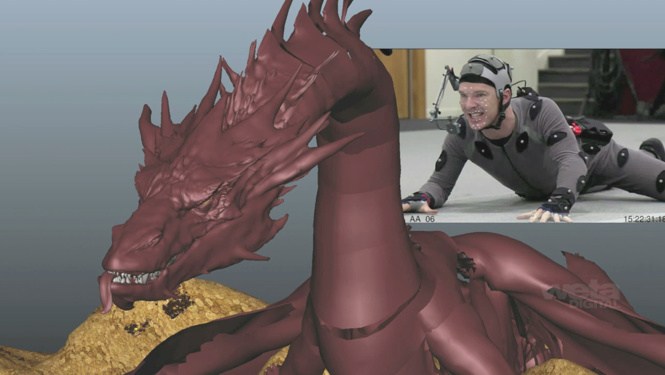
\includegraphics[width=0.4\linewidth]{./figs/exemploSmaug.jpg}}
  \end{subfigure}   
   \begin{subfigure}[]{\label{fig:smaugB}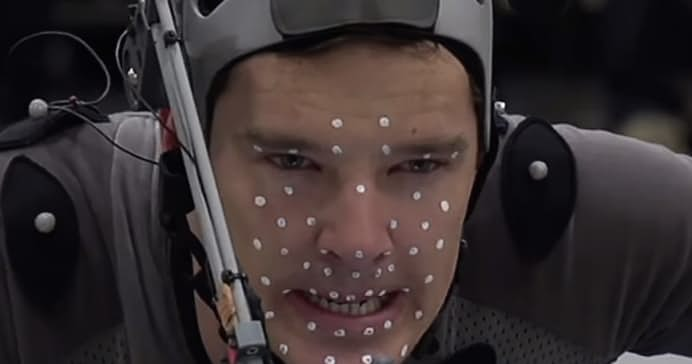
\includegraphics[width=0.4\linewidth]{./figs/Smaug_Benedict.jpg}}
  \end{subfigure}   
    \caption{Exemplo de utilização de captura de movimentos e expressões 
    na indústria cinematográfica. Pontos cuidadosamente colocados no rosto
  do ator são utilizados para transferir expressões para o modelo 
  tridimensional do personagem (retirado de \cite{sherlocksmaug}).}
    \label{fig:smaug}
\end{figure*}

Nesse tipo de aplicação cinematográfica requer-se do sistema de animação
computacional uma alta precisão no ajuste do modelo computacional ao ator em
cena. Para esse fim, utilizam-se ambientes especiais onde a iluminação é
controlada e marcadores visuais no cenário e no ator, sendo que muitas vezes a
captura da imagem é feita por um arranjo de câmeras ou ainda por câmeras de alta
resolução. Além disso, o resultado do processamento recebe um ajuste fino
realizado por vários artistas para que o resultado apresentado seja o mais
convincente possível. Vale notar que não é possível realizar esse ajuste fino
caso não haja um longo prazo disponível entre a captura da imagem e o instante
em que os resultados precisam ser apresentados ao público.

Outro recurso utilizado para a animação auxiliada por captura de vídeo é o uso
de fantoches digitais, mas neste caso os requisitos de tempo são muito mais
severos. Nessa aplicação, vista em programas televisivos e em parques de
diversão ao redor do mundo, um ator em uma câmera escondida anima em tempo real
um modelo renderizado em projetor e responde ao vivo às perguntas do público. O
personagem animado apresenta expressões corporais e faciais que encantam o
público, deixando os mais novos convencidos de que conversaram com seu
personagem preferido e os mais velhos se perguntando como aquilo pode ser
possível. Nessa aplicação, os requisitos de tempo são muito mais severos, devido
ao tempo de resposta curto necessário para a interação entre público e
personagem digital, não é possível o ajuste fino dos artistas, mas ainda sim é
possível fazer uso de iluminação controlada, câmera(s) de alta qualidade e
marcadores visuais. A equipe por trás do personagem pode ainda fazer uso de
controles pré-programados.

Apesar das soluções existentes apresentarem resultados adequados para as
aplicações citadas, elas apresentam um alto custo. Dessa forma, ainda que
grandes empresas se disponham a bancar o preço da tecnologia atual, ele se torna
proibitivo para aplicações desenvolvidas por pequenas empresas. Portanto, o
surgimento de produtos que realizem as mesmas tarefas a custos mais baixos é
certamente de interesse do mercado global de animação. Tal produto poderia, por
exemplo, ser utilizado por animadores independentes para acelerar seus projetos.
A motivação inicial deste trabalho foi justamente a de atender esses animadores
independentes.

Pode-se observar, ainda, que programas de televisão educacionais para crianças
abundam no mercado, mas são em sua maioria direcionados ao público infantil
geral. Um nicho não atendido é o de crianças autistas. Apesar das dificuldades
encontradas por essas crianças variarem muito de um indivíduo para o outro, é
comum que crianças autistas apresentem dificuldade em manter contato visual,
mesmo que seja com personagens de um filme. Assim sendo, as animações
convencionais não são adequadas para esse público e há certamente motivação para
o desenvolvimento de desenhos infantis próprios para as crianças autistas.

Uma empresa interessada em desenvolver tais animações muito provavelmente não
objetiva fins lucrativos, mas sim busca realizar um interesse social. Logo, a
empresa dificilmente terá os mesmos recursos financeiros de uma que trabalhe com
o público geral e não poderá arcar com os custos envolvidos.  Uma das motivações
deste trabalho é que o produto desenvolvido possa ser utilizado como ferramenta
para auxiliar o desenvolvimento de programas infantis com foco em crianças
autistas.

O Capítulo 2 deste trabalho discorre sobre a fundamentação teórica por trás das
técnicas utilizadas. Reconhecimento de pontos do rosto, renderização de objetos
tridimensionais, filtragem digital e estimação de profundidade são tópicos
abordados. No Capítulo 3 as técnicas introduzidas são relacionados para compor a
metodologia da aplicação proposta neste trabalho.  No Capítulo 4 os resultados
obtidos são apresentados e discutidos.  O último capítulo elabora conclusões e
aponta propostas de melhorias futuras para o trabalho.


\chapter{Fundamentos\label{chap:FundamentacaoMatematica}}

% Resumo opcional. Comentar se não usar.
Esta seção introduz os conceitos por trás das técnicas utilizadas no sistema
de animação computacional proposto neste trabalho. O objetivo deste capítulo 
é introduzir o necessário da teoria das técnicas utilizadas, 
para que se entenda as propriedades dosresultados obtidos. A aplicação 
consiste do encadeamento de diversas técnicas oriundas dos domínios de 
Visão Computacional, Geometria Computacional e Filtragem Digital. Como frequentemente
acontece, as técnicas de Visão Computacional muitas vezes empregam conceitos de 
Aprendizado de Máquina. 


\section{Definições Básicas}

\begin{itemize}
\item Imagem

Uma imagem pode ser definida como uma função bidimensional, $\mathpzc{f}(x,y)$,
onde $x$ e $y$ são coordenadas espaciais e a amplitude de $\mathpzc{f}$ em
qualquer par de coordenadas $(x,y)$ é dita a intensidade ou intensidade de cinza
da imagem naquele ponto. Quando $x$, $y$ e o os valores de intensidade de
$\mathpzc{f}$ são todos finitos e discretos, diz-se que a imagem é uma uma
imagem digital. Uma imagem digital é composta de um número finito de elementos,
cada um destes possuindo um valor e uma localização particular. Estes elementos
são mais comumente chamados de pixeis \cite{gonzalesDigitalImageProc}.

\item Sequência de Imagens

Uma sequência de imagens é uma função tridimensional $\mathpzc{h}(x,y,t)$ que
possui uma ou mais imagens $\mathpzc{f}(x,y)$ tomadas em instantes de tempo
discretos $t$ \cite{def:imageSequence}.

\item Rastreamento

Rastreamento é o problema de inferir o movimento de um objeto dada uma sequência
de imagens. Em um problema típico de rastreamento, tem-se um modelo para o
movimento do objeto e um conjunto de medidas oriundas de uma sequência de
imagem. Não é garantido que essas medidas sejam relevantes, podendo elas conter
informação de outros objetos que não o objeto de interesse
\cite{computer-vision-modern-approach-forsithy}.

\end{itemize}


\section{Ajuste de Modelo Deformável}

Ajuste de Modelo Deformável é o problema de ajustar os parâmetros de um modelo
paramétrico a uma imagem de forma que os pontos chaves correspondam com
localizações do objeto de interesse. É uma tarefa difícil uma vez que envolve
uma otimização em um espaço de alta dimensão, no qual a forma de um objeto pode
variar drasticamente entre instâncias do objeto devido a condições de
iluminação, ruído na imagem, resolução e fontes intrínsecas de variabilidade
\cite{saragih2011deformable}.

Ainda segundo \cite{saragih2011deformable}, uma das abordagens mais proeminentes
para o problema consiste em modelar um objeto utilizando observações
espaço-temporalmente coerentes de imagens locais (\textit{image patches})
centradas nos pontos de interesse dentro do objeto. Nesta abordagem, assume-se
que os \textit{patches} são condicionalmente independentes uns dos outros para
fins computacionais e de generalização da técnica. Os detectores locais são
tipicamente aprendidos, a partir de imagens marcadas de treinamento, para cada
ponto proeminente do objeto.

A Figura \ref{fig:pontos-de-interesse} mostra pontos de interesse que podem ser
utilizados em um modelo deformável para a face humana.

Devido ao pequeno suporte destes detectores e a alta variabilidade de aparência
nos dados de treinamento, estes detectores locais estão fadados à ambiguidade
\cite{saragih2011deformable}. 

\begin{figure*}[!htb]
   \centering
\begin{tabular}{cc}
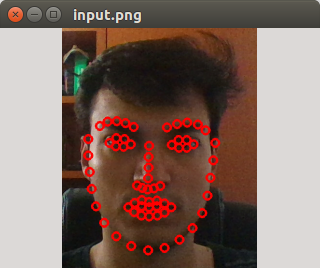
\includegraphics[width=0.4\linewidth]{./figs/sample-detection.png}&
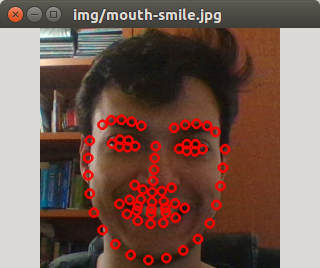
\includegraphics[width=0.4\linewidth]{./figs/sample-detection-2.png}
\end{tabular}
    \caption{Exemplo de regiões de interesse que devem ser marcadas em uma imagem.}
    \label{fig:pontos-de-interesse}
\end{figure*}

\subsection{Ajuste de Modelo Deformável por Deslocamento Regularizado de Média de Pontos Chaves}

O ajuste de modelo deformável por Deslocamento Regularizado de Média de Pontos
Chaves, do inglês \nomenclature{RLMS}{\textit{Regularized Landmark
Mean-Shift}}{\textit{Regularized Landmark Mean-Shift} (RLMS) é uma técnica que
trata o problema de ajuste de modelo deformável empregando sinergicamente as
informações de cada detector local não paramétrico dos pontos proeminentes
\footnote{Ao longo do texto os termos `pontos chave', `pontos proeminentes',
`pontos de interesse' e `marcadores' são sinônimos e referem-se ao conjunto de
pontos rastreados do modelo deformável.} , enquanto limita o efeito de suas
ambiguidades ao ajustar os parâmetros do modelo deformável.

Como é visto a seguir, o modelo deformável paramétrico consiste em um conjunto
de pontos chaves do objeto de interesse. Para cada um desses pontos chaves, o
RMLS utiliza um detector treinado independentemente dos demais. Treiná-los assim
é mais fácil, mas os detectores aprendidos são ruidosos e muitas vezes produzem
resultados ambíguos. O RMLS é uma técnica que permite utilizar as informações de
todos os outros rastreadores para detectar a posição de um ponto proeminente e
não só o rastreador que foi treinado para aquele ponto em específico. Em um
problema de detecção facial, por exemplo, pode-se pensar que se o rastreador
para nariz está em dúvida sobre qual de dois pontos é, mais certamente, o centro
de um nariz, ele pode utilizar informação dos rastreadores dos olhos e da boca
para escolher qual dos dois pontos melhor representa o nariz. 

O exemplo anterior deve ser entendido como uma motivação para a utilização
sinérgica de rastreadores e não mais do que isso. O RLMS é uma técnica de
propósito geral e não assume nenhuma forma para o modelo ou mesmo requer que a
forma como os pontos se arranjam seja informada explicitamente como entrada. O
RLMS aprende conformações prováveis para o conjunto de pontos a partir de dados
de treinamento e poderia ser utilizado tanto para detectar pontos da face humana
como pontos no contorno de um carro. A única diferença seriam os dados de
entrada e, consequentemente, as matrizes aprendidas no processo. 

Quando requerido para ajustar o modelo paramétrico a uma imagem de entrada,
pode-se dizer simplificadamente que o RMLS tentará buscar na imagem de entrada
uma combinação das configurações com as quais ele já foi familiarizado. Como em
muitos outros métodos de Aprendizagem de Máquina, a busca pelos parâmetros que
melhor se adequam é realizada por meio de um processo de otimização de uma
equação de probabilidade. Como parte do objetivo desta fundamentação teórica,
alguns detalhes do RLMS serão apresentados.



\subsection{Modelo de Distribuição de Pontos}

Essa seção especifica o modelo paramétrico utilizado pelo RLMS. O Modelo de
Distribuição de Pontos, do inglês \nomenclature{PDM}{\textit{Point Distribution
Model}} \textit{Point Distribution Model} (PDM), propõe que o objeto a ser
entendido deve ser caracterizado como um conjunto de pontos chaves
bidimensionais no domínio da imagem. O PDM modela linearmente variações de forma
não-rígidas e as compõe com uma transformação rígida global, colocando o i-ésimo
ponto de interesse $\bm{v_i}$ em:

\begin{equation}
 \bm{v_i} = s \bm{R} ( \bm{v}_{i,0} + \bm{\Phi}_i \bm{q}) \bm{t}
\label{eq:PDM-equation}
\end{equation}
 
onde $\mathbf{p}=\{s,\bm{R},\bm{t},\bm{q}\}$ denota os parâmetros do modelo e
consiste do fator de escala $s$, da matriz de rotação $\bm{R}$, do vetor de
translação $\bm{t}$ e de um conjunto de parâmetros não rígidos $\bm{q}$. É esse
conjunto $\mathbf{p}$ que deve ser calculado ao ajustar o modelo a uma imagem
dada, todos os outros termos da equação podem ser previamente calculados em um
processo conhecido como treinamento.  Na Equação \ref{eq:PDM-equation}
$\bm{v_{i,0}}$ denota a posição neutra do $i$-ésimo ponto de interesse e
$\bm{\Phi_i}$ é uma submatriz da base de variações previamente aprendida
pertinente ao $i$-ésimo ponto de interesse.  Nesta equação o termo $\bm{\Phi}_i
\bm{q}$ corresponde à transformação não rígida e os outros termos à
transformação rígida. Nota-se que o modelo consiste de \textbf{uma transformação
rígida aplicada a uma transformação não rígida}. Parte da riqueza do modelo está
na transformação não rígida, que é apresentada mais a fundo a seguir.

O vetor parâmetros não rígidos $\bm{q} \in \realnumbers ^d$ indica o peso com o
qual cada uma das $d$ possíveis transformações não-rígidas influencia o
posicionamento do ponto chave em questão no quadro considerado. O número $d$
deve ser fixado e é referenciado na literatura como a dimensão do PDM. A matriz
$\bm{\Phi}$ contém as $d$ deformações possíveis para cada um dos $K$ pontos de
interesse e a matriz $\Phi_i$ é a submatriz que contém as deformações possíveis
para o $i$-ésimo ponto de interesse.

As constantes $v_{i,0}$ e $\Phi_i$ devem ser aprendidas a partir de um conjunto
de dados de treinamento. O conjunto de dados de treinamento consiste em uma
série de imagens anotadas onde todos os $K$ pontos do PDM foram
\textbf{manualmente} marcados. A partir dessas imagens é possível conhecer as
principais maneiras com que o modelo de pontos aparece deformado na imagem. A
técnica com a qual aprende-se a matriz $\bm{\Phi}$ é a Análise de Componentes
Principais.

Finalmente, nota-se que a Equação \ref{eq:PDM-equation} define $\mathbf{v}_i$
como função de $\mathbf{p}$. A seguinte expansão em série de Taylor é utilizada
para aproximar os valores $\mathbf{v}_i$ em torno de um ponto $\mathbf{v}_i^c$:

\begin{equation}
\mathbf{v}_i \approx \mathbf{v}_i^c + \mathbf{J}_i \Delta \mathbf{p}
\label{eq:alg2}
\end{equation}


\subsection{Análise de Componentes Principais}

A técnica de Análise de Componentes Principais, do inglês
\nomenclature{PCA}{\textit{Principal Components Analysis}} \textit{Principal
Components Analysis} (PCA), é comumente utilizada para reduzir a dimensionalidade
de um conjunto de vetores de características. Um vetor de características é
simplesmente um vetor cujas componentes representam características de um
objeto.  A entrada para a técnica consiste de um conjunto $\mathcal{D}$ de $N$
vetores $D$-dimensionais e a saída é um outro conjunto $D_{PCA}$ de $N$ vetores
$L$-dimensionais. A técnica reduz a dimensionalidade dos dados quando $L < Q$. A
PCA permite isso ao reescrever cada elemento $\bm{v}$ de $D$ como uma combinação
linear de $L$ vetores $D$ dimensionais $\{ \mathbf{w}_1, \mathbf{w}_2, \cdots,
\mathbf{w}_L\}$.  Os pesos $\{z_i\}_{i=1}^L$da combinação se tornam as $L$
componentes do vetor $\mathbf{z} \in \mathcal{D}_{PCA}$. Se a transformação for
perfeita, é possível recuperar unicamente o vetor $\mathbf{v}$ apartir de
$\mathbf{z}$, mas esse não é o caso comum. Em geral a diminuição de dimensão
implica em perda de dados e é possível medir o erro da aproximação. 

Seja $\mathbf{z} = (z_1, z_2, \cdots, z_L)$ um elemento de $D_{PCA}$, uma
estimativa $\mathbf{\hat{v}}$ do vetor $\mathbf{v}$ de $D$ que gerou
$\mathbf{z}$ por meio da transformação é

\begin{equation}
\mathbf{\hat{v}} = z_1 \mathbf{w}_1 + z_2 \mathbf{w}_2 + \cdots + v_L \mathbf{w}_L
\end{equation}

na qual os vetores $w_i, i = 1 \cdots L$ são os vetores base aprendidos pela
PCA. O erro quadrático da transformação é dada por

\begin{equation}
erro_i = ||(\mathbf{\hat{v}}_{i} - \mathbf{v}_i)||^2
\end{equation}

E o erro quadrático médio (a função custo a ser otimizada) para o conjunto de
dados de aprendizagem $\mathcal{D}$ de N elementos $\mathbf{v_i}$ é

\begin{equation}
J(\mathbf{W}, \mathbf{Z} ) = \frac{1}{N}\sum_{i=1}^N ||\mathbf{\hat{v}}_{i} - \mathbf{v}_i||^2
\end{equation}

Onde $\mathbf{W}$ é a matriz obtida concatenado-se os vetores $\mathbf{w}_i$ e
$\mathbf{Z}$ a matriz obtida concatenando-se os $\mathbf{z}_i$. Se $L = D$ então
$E_{total} = 0$ e, geralmente, se $L < D$, $E_{total} > 0$.  Além disso, os
vetores $\mathbf{w}_i$ devem ser ortonormais.

A solução ótima para o problema é conhecida e é encontrada fazendo-se
$\mathbf{W} = \mathbf{V}_L$, onde $\mathbf{V}_L$ contém os L autovetores com
maiores autovalores da matriz empírica de covariância dada por 

\begin{equation}
\hat{\mathbf{\Sigma}} = \frac{1}{N}\sum_{i=1}^{N} \mathbf{v_i}\mathbf{v_i}^T
\end{equation}

Além disso, os $\mathbf{z_i}$ podem ser escritos como $\mathbf{z}_i =
\mathbf{W}^T \mathbf{v}_i$ \cite{machine-learning-book}. Para referências
futuras, nota-se o autovalor associado ao autovetor $\mathbf{w}_i$ por
$\lambda_i$.

A redução de dimensionalidade obtida pela PCA é valiosa por si só, tornando
alguns problemas tratáveis computacionalmente. No entanto, não é com esse
objetivo que a PCA entra no algoritmo utilizado para rastreamento de pontos de
interesse. Para  RLMS, o interesse está nos vetores $\mathbf{w}_i$. Esses
vetores representam as componentes fundamentais escondidas por trás do conjunto
de dados de aprendizado. O conjunto de vetores $\mathbf{w}_i$ é utilizado para
montar a matriz $\Phi$ das transformações permitidas em nosso PDM.

A Figura \ref{fig:PCA} mostra um exemplo em baixa dimensão da técnica de PCA. Os
círculos azuis são os dados originais $\mathbf{v_i}$ e as cruzes vermelhas são
as reconstruções $\mathbf{z_i}$. Observa-se que os pontos são projetados
ortogonalmente sobre a linha que marca a direção principal dada por
$\mathbf{w}_1$ \cite{machine-learning-book}.


\begin{figure*}[!htb]
    \centering
    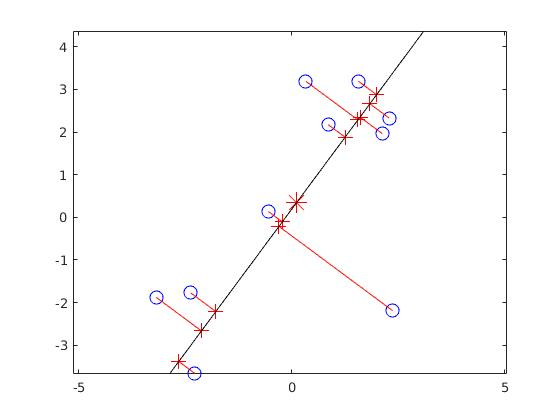
\includegraphics[width=0.8\linewidth]{./figs/pcaDemo.jpg}
% 
    \caption{Imagem retirada de \cite{machine-learning-book}. Exemplo de PCA com D = 2 e L = 1.}
    \label{fig:PCA}
\end{figure*}





\subsection{Conceitos de Probabilidade e Estatística}
\label{ssec:review-probabilidade}

Esta seção apresenta uma breve revisão de conceitos estatísticos necessários
para se entender a formulação na Seção \ref{ssec:tracking-parameter-fitting}.

\begin{itemize}

\item Variável Aleatória

Uma variável aleatória é uma variável cujos possíveis valores são resultados
numéricos de um fenômeno aleatório. Uma variável aleatória discreta é aquela
restrita a assumir valores dentre um conjunto contável de eventos. No texto que
segue, uma variável aleatória $\varkappa$ assume valores em um conjunto
$\Upsilon = \{\varphi_1, \varphi_2, \ldots\}$.

\item Probabilidade

Diz-se que a probabilidade da ocorrência de um evento é uma medida da confiança
que ele ocorra. A probabilidade é um número real entre 0 (indicando
impossibilidade) e 1 (indicando certeza). Quanto maior a probabilidade de um
evento, mais certeza há sobre sua ocorrência. No texto que segue, $\varkappa_1$
e $\varkappa_2$ são duas variáveis aleatórias, cada uma tomando valores em
$\Upsilon _1 = \{\varphi_1^1, \varphi_1^2, \ldots\}$ e $\Upsilon_2 =
\{\varphi_2^1, \varphi_2^2, \ldots\}$. Denota-se a probabilidade que
$\varkappa_1$ assuma valor $\varphi_1 \in \Upsilon_1$ como
$\mathpzc{p}(\varkappa_1 = \varphi_1)$ ou simplesmente $\mathpzc{p}(\varphi_1)$.

\item Probabilidade Conjunta

A probabilidade conjunta para $\varkappa_1$ e $\varkappa_2$ é a distribuição de
probabilidade que informa a probabilidade que $\varkappa_1 = \varphi_1$ e
$\varkappa_2 = \varphi_2$, $\forall (\varphi_1, \varphi_2) \in \Upsilon_1 \times
\Upsilon_2$, representada por $\mathpzc{p}(\varphi_1, \varphi_2)$. A definição
pode ser expandida para $k$ variáveis. Pode-se com isso definir a probabilidade
de um vetor discreto aleatório $k$-dimensional $\mathbf{\varkappa} =
[\varkappa_1, \ldots, \varkappa_k]$ como:

\begin{equation}
\mathpzc{p}(\mathbf{\varkappa}) = \mathpzc{p}(\varkappa_1, \varkappa_2, \ldots, \varkappa_k) 
\end{equation}

\item Probabilidade Condicional

Probabilidade condicional é a medida de probabilidade de um evento dado que um
outro evento ocorreu. A probabilidade condicional de $\varphi_1$ dado
$\varphi_2$ é escrita como $\mathpzc{p}(\varphi_1 | \varphi_2)$ e pode ser
calculada por:

\begin{equation}
\mathpzc{p}(\varphi_1 | \varphi_2) = \frac{\mathpzc{p}(\varphi_1, \varphi_2)}{\mathpzc{p}(\varphi_2)}
\end{equation}


\item Marginalização

Suponha que um dado processo estocástico seja governado por uma função de
probabilidade $\mathpzc{p}(\varphi_1,\varphi_2)$.  Suponha ainda que em dada
aplicação $\varphi_1$ seja uma variável de interesse e não se dê importância
para $\varphi_2$. Pode-se calcular a probabilidade $\mathpzc{p}(\varphi_1)$ ao
marginalizar-se $\varphi_2$:

\begin{equation}
\mathpzc{p}(\varphi_1) = \sum_{\varphi_2 \in \Upsilon_2} \mathpzc{p}(\varphi_1|\varphi_2)\mathpzc{p}(\varphi_2)
\end{equation}

\item Lei de Probabilidade Total

O seguinte resultado combina marginalização e probabilidade condicional:

\begin{equation}
\mathpzc{p}(\varphi_1|\varphi_3) = \sum_{\varphi_2 \in \Upsilon_2} \mathpzc{p}(\varphi_1|\varphi_2, \varphi_3)\mathpzc{p}(\varphi_2|\varphi_3)
\end{equation}

\item Distribuição Normal Multivariada

Uma função que comumente aparece em estatística é a distribuição normal. A
distribuição normal, ou gaussiana, em várias dimensões é escrita como:

\begin{equation}
\mathpzc{p}(\mathbf{\varphi}) = (2\pi)^{-\frac{k}{2}} | \mathbf{\Sigma} | ^ {-\frac{1}{2}} e^{-\frac{1}{2}(\mathbf{\varphi} - \mathbf{\mu})'\mathbf{\Sigma}^{-1}(\mathbf{\varphi} - \mathbf{\mu})}
\end{equation}

onde $\mathbf{\Sigma}$ é a matriz de co-variâncias e $\mathbf{\mu}$, um vetor
k-dimensional, é a média da distribuição. Quando uma variável k-dimensional
$\mathbf{\varkappa}$ possui distribuição de probabilidade dada por uma gaussiana
de média $\mathbf{\mu}$ e covariância $\mathbf{\Sigma}$, a seguinte notação é
utilizada:

\begin{equation}
\mathbf{\varkappa} \sim \mathcal{N}(\mathbf{\varkappa}; \mathbf{\mu}, \mathbf{\Sigma})
\end{equation}

A Figura \ref{fig:normal} mostra a forma de sino da Gaussiana bidimensional.

\begin{figure}[!htbp]
\centering
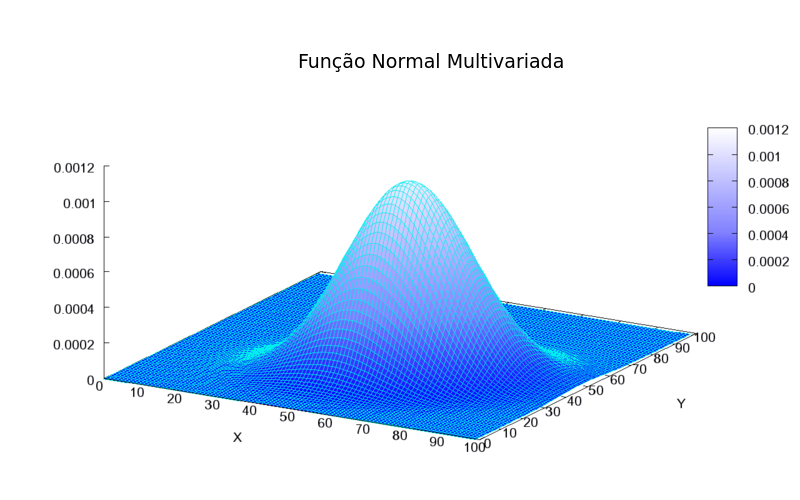
\includegraphics[width=0.7\textwidth]{figs/multivariate.png}
\caption{Distribuição Normal Bidimensional.}
%https://en.wikipedia.org/wiki/Multivariate_normal_distribution\
\label{fig:normal}
\end{figure}

\end{itemize}

\subsection{Formulação Estatística para o Ajuste de Parâmetros}
\label{ssec:tracking-parameter-fitting}

Como visto anteriormente, ajustar o PDM a uma imagem significa calcular o
conjunto $\mathbf{p} = \{s, \bm{R}, \bm{t}, \bm{q}\}$ que melhor ajusta o modelo
à imagem que se quer ajudar. Isso é feito minimizando-se a função custo

\begin{equation}
Q(\mathbf{p}) = R(\mathbf{p}) + \sum_{i=1}^n D_i(\mathbf{v}_i; \mathcal{I})
\label{eq:objective-function}
\end{equation}

na qual R é um fator de regularização que penaliza deformações complexas e $D_i$
denota uma medida de desalinhamento para o i-ésimo ponto de interesse na imagem
I \cite{facetracker}.

A Equação \ref{eq:objective-function} pode ser interpretada probabilisticamente
como a maximização da probabilidade dos parâmetros do modelo de forma que os
pontos de interesse estejam alinhados com suas respectivas localizações no
objeto em uma imagem \cite{facetracker}. A forma da função custo na Equação
\ref{eq:objective-function} assume implicitamente independência condicional
entre a detecção de cada ponto chave. Probabilisticamente falando, essa
independência condicional toma a forma:

\begin{equation}
\label{eq:conditional-independence}
\mathpzc{p}(\mathbf{p} | \{l_i = 1\}_{i=1}^n, \mathcal{I}) \varpropto \mathpzc{p}(\bf{p}) \prod_{i=1}^n \mathpzc{p}(l_i = 1 | \mathbf{v}_i, \mathcal{I})
\end{equation}

A variável discreta $l_i \in \{1, -1\}$ indica se o i-ésima ponto chave está
alinhado ou desalinhado, sendo $l_i=1$ no primeiro caso e $l_i=-1$ no segundo.
Na Equação \ref{eq:conditional-independence} o símbolo $\varpropto$ indica que
existe uma relação de proporção direta entre os termos a esquerda e a direita do
símbolo. Deixando mais claro, a notação $\mathpzc{a} \varpropto \mathpzc{b}$
significa que $\exists k \in \mathbb{R}$ tal que $\mathpzc{a} = k \mathpzc{b}$.
Como se está falando de probabilidade, vale notar que a constante deve ser
positiva e, portanto, maximizar o lado direito implica em maximizar o lado
esquerdo da Equação \ref{eq:conditional-independence}.  Para se obter a Equação
\ref{eq:objective-function}, aplica-se o logaritmo em ambos os lados da Equação
\ref{eq:conditional-independence} para transformar os produtos em somatório.
Além disso, algoritmos de otimização são comumente escritos para minimizar
funções e não para as maximizar. Por esse motivo, inverte-se o sinal da equação
obtida de forma que maximizar $f(\mathbf{x})$ é o mesmo que minimizar
$-f(\mathbf{x})$. Obtém-se então uma forma para as componentes de Q na Equação
\ref{eq:objective-function}:

\begin{equation}
\label{eq:P}
P(\mathbf{p}) = 
-\ln
(
\mathpzc{p}(\mathbf{p})
)
\end{equation}

\begin{equation}
D(\mathbf{v}_i; I) =
-\ln
(
\mathpzc{p}(l_i=1 | \mathbf{x}_1, \mathcal{I})
)
\end{equation}

Em \cite{facetracker}, utiliza-se a seguinte função para a probabilidade de alinhamento de uma localização $\bf{x}$ de um ponto chave: 

\begin{equation}
p(l_i = 1|\textbf{v},\mathcal{I}) = \frac{1}{1 + \exp{\{}l_iC_i(\textbf{v};\mathcal{I}){\}}}
\label{eq:alg1}
\end{equation}

Sendo $C_i$ o classificador que distingue locações alinhadas de desalinhadas
\cite{saragih2011deformable}. Ainda em \cite{facetracker}, o classificador $C_i$
utilizado é um de regressão logística aplicado em uma janela $\bf{\Omega_x}$ de
pixeis ao redor de $\bf{x}$.

Para completar a abordagem é preciso especificar $p(\bf{p})$ em \ref{eq:P}. Este
termo indica um conhecimento prévio sobre a distribuição dos parâmetros. Quando
se assume que todas as configurações são igualmente prováveis a formulação em
\ref{eq:conditional-independence} leva a uma estimação dos parâmetros \textbf{p}
por maximização de probabilidade, ou, em inglês, \textit{Maximum Likelihood}.
Quando, por outro lado, supõe-se uma distribuição não uniforme dos parâmetros,
tem-se uma estimação de Máximo a Priori (MAP) \cite{saragih2011deformable}.
Lembrando que para o MDP $\mathbf{p}=\{s,\mathbf{R},\mathbf{t},\mathbf{q}\}$,
$\mathpzc{p}(\mathbf{p})$ é especificado por partes. Em geral, assume-se um
modelo gaussiano para os parâmetros não rígidos $\mathbf{q}$ e uma probabilidade
uniforme sobre os parâmetros rígidos $\{s,\mathbf{R},\mathbf{t}\}$
\cite{facetracker}. O que leva a distribuição a priori:

\begin{equation}
\mathpzc{p}(\mathbf{p}) \varpropto \mathcal{N}(\mathbf{q}; 0, \mathbf{\Lambda})
\label{eq:Lambda}
\end{equation}

com $\mathbf{\Lambda} = \text{diag}\{[ \lambda_1; \ldots; \lambda_m]\}$, isto é,
a matriz diagonal contendo os autovalores dos modos de deformação aprendidos
pelo PCA. Nota-se que quanto maior o valor de $\lambda_i$ mais lentamente decai
a distribuição normal em \ref{eq:Lambda}. Colocando de outra forma, um maior
$\lambda_i$ indica que é mais provável uma componente $p_i$ em $\mathbf{p}$ de
alta magnitude.


\subsection{Otimização de Probabilidade por Deslocamento Regularizado de Média}

Devido ao erro de truncamento herdado do PCA, o modelo utilizado não pode
reconstruir perfeitamente a localização perfeita das poses chaves
\cite{saragih2011deformable}. O erro de truncamento é modelado nesta técnica
por:

\begin{align}
y_i = x_i + \epsilon_i
\label{eq:erro-trunc}
\end{align}

sendo $\epsilon_i \sim \mathcal{N}(\epsilon_i; 0, \rho I)$, $y_i$ a variável
aleatória representando a posição real da i-ésima pose chave e o parâmetro
$\rho$ pode ser aprendido durante o treinamento. A Equação \ref{eq:erro-trunc}
nos dá uma forma para $p(y_i | x_i)$:

\begin{equation}
p(y_i | v_i) = N(y_i; v_i, \rho I)
\end{equation}

Para a próxima etapa assume-se que existe um conjunto de candidatos $\Phi_i$
para cada marcador i do modelo. Por exemplo $\Phi_i$ pode denotar os pontos em
uma região de busca pelo i-ésimo ponto chave. Tratando a localização real dos
marcadores $y_i$ como uma variável escondida, pode-se marginalizá-la da
probabilidade de alinhamento dos marcadores:

\begin{equation}
p(l_i = 1|v_i, I) = \sum_{y_i \in \Phi_i} p(l_i = 1| y_i, \mathcal{I})p(y_i|v_i)
\end{equation}

O termo $p(l_i = 1| y_i, \mathcal{I})$ é renomeado $\pi_{y_i}$ e a equação é reescrita:

\begin{equation}
\label{eq:eq32}
p(l_i = 1|\mathbf{v}_i, \mathcal{I}) = \sum_{\mathbf{y}_i \in \mathbf{\Phi}_i} \pi_{\mathbf{y}_i} N(\mathbf{v}_i; \mathbf{y}_i, \rho \mathcal{I})
\end{equation}

Substituindo \ref{eq:eq32} em \ref{eq:conditional-independence}
 obtém-se:

\begin{equation}
p(p|\{l_i=1\}_{i=1}^n, \mathcal{I}) \varpropto p(p) \prod_{i=1}^n \sum_{\mathbf{y}_i \in \mathbf{\Phi}_i}
\pi_{y_i} N(\mathbf{v}_i; \mathbf{y}_i, \rho \mathbf{I})
\label{eq:eq23}
\end{equation}

A Equação \ref{eq:eq23} pode ser minimizada por um processo iterativo que
envolve calcular o vetor deslocamento de média $v = [v_1, v_2, \ldots, v_n]$ e a
atualização dos parâmetros $\Delta p$ através de:

\begin{equation}
\textbf{v}_i = \Bigg(\sum\limits_{\textbf{y}_i \in \Psi_i} \frac{\pi_{\textbf{y}_i}\mathcal{N}(\textbf{v}_i^c;\textbf{y}_i,\rho\textbf{I})}{\sum\nolimits_{\textbf{z}_i \in \Psi_i} \pi_{\textbf{z}_i}\mathcal{N}(\textbf{v}_i^c;\textbf{z}_i,\rho\textbf{I})
}\textbf{y}_i\Bigg) - \textbf{v}_i^c
\label{eq:alg3}
\end{equation}

e

\begin{equation}
\Delta\textbf{p} = -(\rho\tilde{\mathbf{\Lambda}}^{-1} + \textbf{J}^T\textbf{J})^{-1}(\rho\tilde{\mathbf{\Lambda}}^{-1}\textbf{p} - \textbf{J}^T\textbf{v})
\label{eq:alg4}
\end{equation}

onde $\tilde{\mathbf{\Lambda}}$ é a matriz diagonal cujos elementos da diagonal
são os elementos do vetor $[\mathbf{0}, \lambda_1, \ldots, \lambda_m]$,
$\mathbf{J} = [\mathbf{J}_1; \ldots; \mathbf{J}_n]$ é o jacobiano do PDM(ver
Equação \ref{eq:PDM-equation}) e $\mathbf{x}_c^i$ é a estimação atual do
$i$-ésimo marcador.




               
\section{Estimação de Profundidade}

Um problema que aparece quando se trata de visão monocular é a falta de
informação de profundidade, uma vez que o processo de formação de uma imagem
consiste na captura apenas de duas das três dimensões espaciais. Com isso, uma
infinidade de objetos tridimensionais podem ser relacionados a uma mesma imagem
bidimensional. Ou seja, uma imagem não contém informações suficientes para
reconstruir uma cena tridimensional \cite{bolles1987epipolar}. No entanto, uma
aplicação que necessite de informação de tridimensionalidade a partir de captura
de imagens pode utilizar duas ou mais câmeras cujos parâmetros intrínsecos são
conhecidos.

\subsection{Modelo da Câmera}

Nesta seção é definido o modelo de câmera necessário para a extração dos
parâmetros intrínsecos utilizados neste trabalho. 

Primeiramente, apresenta-se o modelo de projeção dos pontos do sistema de
coordenadas do mundo para o plano da imagem. Considera-se que o centro da
projeção é a origem do sistema de coordenadas e que $\{(X,Y,Z), Z = f\}$
corresponde ao plano da imagem. Usando um modelo de câmera \textit{pinhole}, um
ponto no sistema de coordenadas do mundo $\mathcal{X} = (X,Y,Z)^T$ é mapeado
para um ponto no plano da imagem como mostrado na Figura \ref{fig:projeção}.

\begin{figure}[h!]
\centering
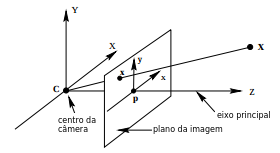
\includegraphics[width=.5\linewidth]{figs/TG_pinhole_1_pt.png}
\caption{Projeção de um ponto no mundo para o plano da imagem (adaptado de \cite{hartley2003multiple}).}
\label{fig:projeção}
\end{figure}

Por aplicação de uma semelhança de triângulos ilustrada na Figura \ref{fig:mapeamento} é possível mostrar que o ponto $(X,Y,Z)^T$ do espaço é mapeado para o ponto $(fX/Z,fY/Z,f)^T$ no domínio da imagem, ou seja:

\begin{equation}
(X,Y,Z)^T \mapsto (fX/Z,fY/Z)^T
\label{eq:3d_mapPonto}
\end{equation}


\begin{figure}[h!]
\centering
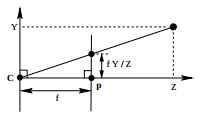
\includegraphics[width=.5\linewidth]{figs/TG_pinhole_2.png}
\caption{Mapeamento de um ponto no mundo para o plano da imagem (retirado de \cite{hartley2003multiple}).}
\label{fig:mapeamento}
\end{figure}

Sendo os pontos no mundo e na imagem representados por vetores homogêneos, então
a projeção central é expressa como um mapeamento linear de suas coordenadas
homogêneas:

\begin{align}
\left(\begin{array}{c}
X\\
Y\\
Z\\
1
\end{array}\right) \mapsto
\left(\begin{array}{c}
fX\\
fY\\
Z
\end{array}\right) =
\left[\begin{array}{cccc}
f & 0 & 0 & 0\\
0 & f & 0 & 0\\
0 & 0 & 1 & 0
\end{array}\right]
\left(\begin{array}{c}
X\\
Y\\
Z\\
1
\end{array}\right)
\label{eq:3d_vetHomogeneo1}
\end{align}

Fazendo $\mathcal{X}$ o vetor homogêneo $(X,Y,Z,1)^T$ e $\mathtt{x}$ o ponto na
imagem representado por um vetor de 3 dimensões, tem se que $\bm{\mathcal{P}}$
representa a matriz de projeção da câmera, sendo que a relação entre esses
termos dada por:

\begin{equation}
\mathtt{x} = \bm{\mathcal{P}}\mathcal{X}
\label{eq:3d_Pmatriz}
\end{equation}

Este mapeamento assume que a origem do sistema de coordenadas no plano da imagem
é a mesma do sistema de coordenadas da câmera; porém, isso nem sempre é verdade
\cite{hartley2003multiple}. Na prática tem-se que:

\begin{equation}
(X,Y,Z)^T \mapsto (fX/Z + p_x,fY/Z + p_y)^T
\label{eq:3d_mapForaCentro}
\end{equation}


sendo $p_x$ e $p_y$ são as coordenadas do \textbf{ponto principal}. Desta forma,
ao expressar em coordenadas homogêneas a equação é:

\begin{align}
\left(\begin{array}{c}
X\\
Y\\
Z\\
1
\end{array}\right) \mapsto
\left(\begin{array}{c}
fX + Zp_x\\
fY + Zp_y\\
Z
\end{array}\right) =
\left[\begin{array}{cccc}
f & 0 & p_x & 0\\
0 & f & p_y & 0\\
0 & 0 & 1 & 0
\end{array}\right]
\left(\begin{array}{c}
X\\
Y\\
Z\\
1
\end{array}\right)
\label{eq:3d_vetHomogeneo2}
\end{align}

Definindo $\bf{K}$ como:

\begin{align}
\bf{K} =
\left[\begin{array}{ccc}
f & 0 & p_x\\
0 & f & p_y\\
0 & 0 & 1
\end{array}\right]
\label{eq:3d_matIntrinseca}
\end{align}

tem-se que $\mathtt{x}$ é dado por:

\begin{equation}
\mathtt{x} = \bf{K}[\bf{I}|0]\mathcal{X}
\label{3d_camModel1}
\end{equation}

A matriz $\bf{K}$ é chamada de matriz intrínseca da câmera.

No geral, pontos no mundo serão expressados como termos de diferentes sistemas
de coordenadas. Isso implica que a origem do sistema de coordenadas do mundo
geralmente não coincide com a origem do sistema de coordenadas da câmera
\cite{hartley2003multiple}, esses dois sistemas de coordenadas são então
relacionados por rotação e translação, como visto na Figura \ref{fig:trans_rot}
.

\begin{figure}[h!]
\centering
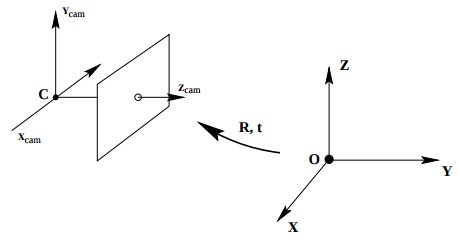
\includegraphics[width=.5\linewidth]{figs/TG_rot_tr.png}
\caption{Transformação entre as coordenadas globais e as coordenadas da câmera por rotação e translação (retirado de \cite{hartley2003multiple}).}
\label{fig:trans_rot}
\end{figure}

Se $\tilde{\mathcal{X}}$ é um vetor não homogêneo que representa um ponto no
sistema de coordenadas do mundo e $\tilde{\mathcal{X}}_{cam}$ representa o mesmo
ponto no sistema de coordenadas da câmera, então pode se dizer que
$\tilde{\mathcal{X}}_{cam} = \bf{R}(\tilde{\mathcal{X}} - \tilde{C})$, onde
$\tilde{C}$ representa o centro da câmera no sistema de coordenadas do mundo e
$\bf{R}$ é a matriz de rotação que representa a orientação do sistema de
coordenadas da câmera. A equação em termos de coordenadas homogêneas pode ser
descrita por:

\begin{align}
\mathcal{X}_{cam} =
\left[\begin{array}{cc}
\bf{R} &  -\bf{R}\tilde{C}\\
0 & 1
\end{array}\right]
\mathcal{X}
\label{eq:3d_matRot}
\end{align}

na qual $\mathtt{x}$ é descrito por:

\begin{equation}
\mathtt{x} = \bf{K}\bf{R}[\bf{I}|-\tilde{C}]\mathcal{X}
\label{eq:3d_camModel2}
\end{equation}

Usando a matriz de projeção da câmera definida na Equação \ref{eq:3d_Pmatriz},
$\bm{\mathcal{P}}$ pode ser escrito como:

\begin{equation}
\bm{\mathcal{P}} = \bf{K}\bf{R}[\bf{I}|-\tilde{C}]
\label{eq:3d_PModel1}
\end{equation}


Este é o modelo básico dado por uma câmera do tipo \textit{pinhole}. É muitas
vezes conveniente não explicitar o centro da câmera \cite{hartley2003multiple},
mas representar a transformação de um ponto no mundo para um ponto na imagem
como $\tilde{\mathcal{X}}_{cam} = \bf{R}\tilde{\mathcal{X}} + \bf{t}$, sendo
$\bf{t} =-\bf{R}\tilde{C}$. Neste caso, a matriz dos parâmetros intrínsecos da
câmera $\bm{\mathcal{P}}$  é escrita como

\begin{equation}
\bm{\mathcal{P}} = \bf{K}[\bf{R}|\bf{t}]
\label{eq:3d_PModel2}
\end{equation}

\subsection{Triangulação}

Para a reconstrução tridimensional da cena, deve se resolver o problema da
triangulação. Supondo que um ponto $\mathcal{X}$ em $R^3$ é visível em duas
imagens e que as distâncias focais $f_1$ e $f_2$ correspondentes a essas duas
imagens são conhecidas, sendo $u$ e $u'$ as projeções do ponto $\mathcal{X}$ nas
imagens, as linhas no espaço correspondentes aos dois pontos da imagem podem
ser, a partir desses dados, facilmente computadas. O problema da triangulação é
achar a interseção destas duas linhas no espaço \cite{hartley1997triangulation}.
Este modelo pode ser visualizado na Figura \ref{fig:disp_cameras}.

\begin{figure}[h!]
\centering
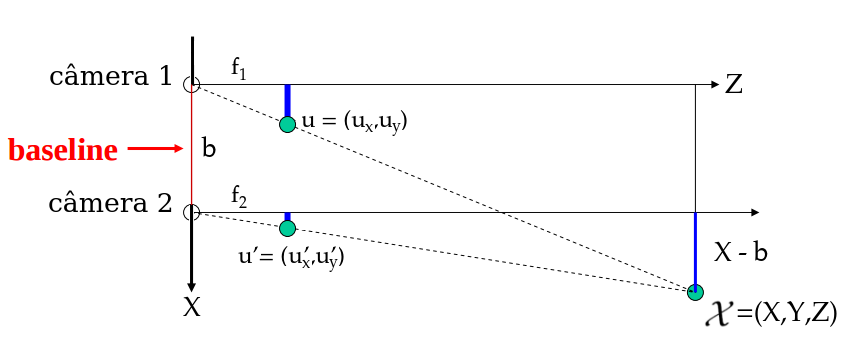
\includegraphics[width=.72\linewidth]{figs/TG_triangulation_pdf_washington_pt2.png}
\caption{Disposição das câmeras (adaptado de \cite{stereovision-washington-pdf}).}
\label{fig:disp_cameras}
\end{figure}

%https://courses.cs.washington.edu/courses/cse455/09wi/Lects/lect16.pdf

Com a Figura \ref{fig:disp_cameras} como referência, é possível, por semelhança
de triângulos, derivar as seguintes equações para o valor $X$ do ponto no
sistema de coordenadas do mundo.

\begin{equation}
X = (u_x/f_1)  Z
\label{eq:3d_realX1}
\end{equation}   

ou

\begin{equation}
X = (u'_x/f_2)  Z + b
\label{eq:3d_realX2}
\end{equation}  

A relação do valor $Y$ do ponto no sistema de coordenadas do mundo pode também
ser relacionado com sua projeção no plano da imagem por uma semelhança de
triângulos, como mostrado na Figura \ref{fig:mapeamento}. As equações de $Y$ são
mostradas a seguir.

\begin{equation}
Y = (u_y/f_1) Z
\label{eq:3d_realY1}
\end{equation}      

ou

\begin{equation}
Y = (u'_y/f_2) Z
\label{eq:3d_realY2}
\end{equation}  


A partir das Equações \ref{eq:3d_realX1} e \ref{eq:3d_realX2} é possível
expressar o valor da profundidade $Z$ do ponto como

\begin{equation}
Z = f_1  f_2  b / (u_x  f_2 - u'_x  f_1)
\label{eq:3d_Zequation}
\end{equation}


Em que $b$ se refere a \textit{baseline}, ou seja, a distância fixa entre as
câmeras, $u'_x$ e $u_x$ são os valores em $x$ da projeção do ponto no plano da
imagem das câmeras 1 e 2, respectivamente, e $f_1$ e $f_2$ são as distâncias
focais obtidas a partir da matriz intrínseca de cada câmera, esta que pode ser
derivada através da matriz da câmera, também chamada de matriz de calibração. A
matriz de calibração pode ser obtida usando a \textit{Calibration Toolbox for
Matlab}, onde a partir de uma série de imagens de um tabuleiro de xadrez
(\textit{chessboard}) capturadas pela mesma câmera é possível relacionar pontos
iguais em várias imagens e então derivar a matriz de calibração
\cite{bouguetML}.

\section{Renderização de Objetos Tridimensionais}

A renderização de objetos tridimensionais neste trabalho foi feita utilizando a
\nomenclature{API}{\textit{Application program interface}} Interface de
Programação de Aplicações (API) \nomenclature{OpenGL}{\textit{Open Graphics
Library}} \textit{Open Graphics Library} (OpenGL). Para a compreensão de como
esta renderização é feita, deve-se entender como é formado um objeto e como ele
é posicionado no sistema de coordenadas. 

Um triângulo é a estrutura mais básica em computação tridimensional
\cite{openGlWikibooks} e todos os objetos neste trabalho são representados
computacionalmente por um conjunto de pequenos triângulos texturizados. Um
triângulo é definido por três vértices e cada vértice é composto por três
coordenadas: $X_p$, $Y_p$ e $Z_p$.
% [wikibooks.org/wiki/OpenGL_Programming/Modern_OpenGL_Introduction]

A informação de um objeto tridimensional completamente renderizado é armazenada
em um \nomenclature{VAO}{\textit{Vertex Array Object}} \textit{Vertex Array
Object} (VAO), uma estrutura que contém um ou mais
\nomenclature{VBO}{\textit{Vertex Buffer Object}} \textit{Vertex Buffer Objects}
(VBOs). Um VBO é um \textit{buffer} de memória contido na memória de alta
velocidade da placa de vídeo, e contém informações sobre os vértices
\cite{openGlOrg}. Podem, por exemplo, conter as coordenadas dos vértices ou
talvez a cor associada a cada vértice.

% [opengl.org/wiki/Tutorial2:_VAOs,_VBOs,_Vertex_and_Fragment_Shaders_(C_/_SDL)]

Desta maneira é possível criar a forma de um objeto construindo um VBO que
contém as coordenadas de todos os triângulos que compõem o objeto; porém, assim
sempre existirão duplicatas quando vértices de dois triângulos compartilharem
uma aresta \cite{openGlTutorial}. Para evitar esta replicação desnecessária, os
pontos em si são guardados separadamente do objeto e a malha é construída com
índices para estes pontos. O efeito desta indexação é ilustrado na Figura
\ref{fig:VBO}.

\begin{figure}[h!]
\centering
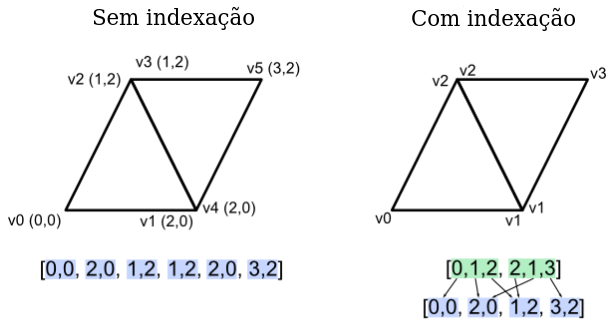
\includegraphics[width=.5\linewidth]{figs/TG_VBO_index_pt.png}
\caption{Indexação do VBO (adaptado de \cite{openGlTutorial}).}
\label{fig:VBO}
\end{figure}

Além disso, esta forma de representação tem a  vantagem de apresentar uma
estrutura bem semelhante a forma como a geometria tridimensional  é armazenada
em um arquivo no formato OBJ. Esta semelhança faz com que o carregamento destes
arquivos para a renderização utilizando OpenGL fique bem mais simples.

Para definir um objeto completamente e não apenas sua forma, se faz necessário o
uso de outros VBOs como, por exemplo, um VBO contendo informações das
coordenadas de textura e um VBO contendo informações das direções normais a
superfície de cada triângulo. A direção normal é importante para que se aplique
iluminação sobre o objeto renderizado e sem iluminação adequada não seria
possível ver os detalhes da superfície, apenas seu contorno.

% [opengl-tutorial.org/intermediate-tutorials/tutorial-9-vbo-indexing/]

Para o posicionamento do objeto no sistema de coordenadas ser definido,
primeiramente são definidas as seguintes matrizes de transformação: translação,
rotação e escala.

A matriz de translação é dada por:

\begin{align}
\left[\begin{array}{cccc}
1 & 0 & 0 & D_y\\
0 & 1 & 0 & D_x\\
0 & 0 & 1 & D_z\\
0 & 0 & 0 & 1
\end{array}\right]
\left(\begin{array}{c}
X_p\\
Y_p\\
Z_p\\
1
\end{array}\right) =
\left(\begin{array}{c}
X_p + D_x\\
Y_p + D_y\\
Z_p + D_z\\
1
\end{array}\right)
\label{eq:rend_translationMat}
\end{align}

A matriz de escala por:

\begin{align}
\left[\begin{array}{cccc}
S_x & 0 & 0 & 0\\
0 & S_y & 0 & 0\\
0 & 0 & S_z & 0\\
0 & 0 & 0 & 1
\end{array}\right]
\left(\begin{array}{c}
X_p\\
Y_p\\
Z_p\\
1
\end{array}\right) =
\left(\begin{array}{c}
S_x \cdot X_p\\
S_y \cdot Y_p\\
S_z \cdot Z_p\\
1
\end{array}\right)
\label{eq:rend_scaleMat}
\end{align}

E as matrizes de rotação:

Rotação no eixo X:

\begin{align}
\left[\begin{array}{cccc}
1 & 0 & 0 & 0\\
0 & cos\theta & -sen\theta & 0\\
0 & sen\theta & cos\theta & 0\\
0 & 0 & 0 & 1
\end{array}\right]
\left(\begin{array}{c}
X_p\\
Y_p\\
Z_p\\
1
\end{array}\right) =
\left(\begin{array}{c}
X_p\\
cos\theta \cdot Y_p - sen\theta \cdot Z_p\\
sen\theta \cdot Y_p + cos\theta \cdot Z_p\\
1
\end{array}\right)
\label{eq:rend_rotationMatX}
\end{align}

Rotação no eixo Y:

\begin{align}
\left[\begin{array}{cccc}
cos\theta & 0 & sen\theta & 0\\
0 & 1 & 0 & 0\\
-sen\theta & 0 & cos\theta & 0\\
0 & 0 & 0 & 1
\end{array}\right]
\left(\begin{array}{c}
X_p\\
Y_p\\
Z_p\\
1
\end{array}\right) =
\left(\begin{array}{c}
cos\theta \cdot X_p + sen\theta \cdot Z_p\\
Y_p\\
-sen\theta \cdot X_p + cos\theta \cdot Z_p\\
1
\end{array}\right)
\label{eq:rend_rotationMatY}
\end{align}

Rotação no eixo Z:

\begin{align}
\left[\begin{array}{cccc}
cos\theta & -sen\theta & 0 & 0\\
sen\theta & cos\theta & 0 & 0\\
0 & 0 & 1 & 0\\
0 & 0 & 0 & 1
\end{array}\right]
\left(\begin{array}{c}
X_p\\
Y_p\\
Z_p\\
1
\end{array}\right) =
\left(\begin{array}{c}
cos\theta \cdot X_p - sen\theta \cdot Y_p\\
sen\theta \cdot X_p + cos\theta \cdot Y_p\\
Z_p\\
1
\end{array}\right)
\label{eq:rend_rotationMatZ}
\end{align}

% [//open.gl/transformations]

Os vértices são aqui definidos como vetores de quatro dimensões pois em OpenGL
este quarto parâmetro, chamado de $W_p$, define se o vetor é uma posição no
espaço, caso $W_p = 1$, ou se o vetor é uma direção, caso $W_p = 0$.

Com essas matrizes definidas pode-se derivar outras três matrizes: a matriz do
modelo, a matriz de visualização e a matriz de projeção. Essas matrizes são
úteis para separar as transformações de forma eficiente.

Um objeto é definido por um conjunto de vértices e as coordenadas $X_p$, $Y_p$ e
$Z_p$ destes vértices são definidos relativamente ao centro do objeto, ou seja,
se um vértice está localizado em $(0,0,0)$, então ele está localizado no centro
do objeto \cite{openGlTutorial}. Para mover o objeto no espaço virtual
utiliza-se a matriz do modelo, que é um produto das matrizes de translação,
rotação e escala aplicadas no objeto. A aplicação desta transformação  coloca
vértices do objeto no sistema de coordenadas do espaço. A Figura
\ref{fig:mat_modelo} ilustra a transformação.

\begin{figure}[h!]
\centering
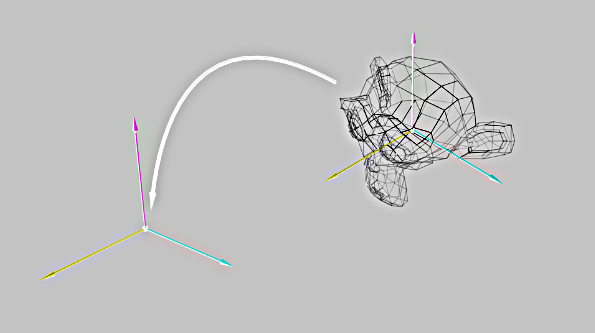
\includegraphics[width=.5\linewidth]{figs/TG_model_matrix_neg.png}
\caption{Efeito da Matriz do Modelo (adaptado de \cite{openGlTutorial}).}
\label{fig:mat_modelo}
\end{figure}

% [opengl-tutorial.org/beginners-tutorials/tutorial-3-matrices/]

A matriz de visualização pode ser interpretada como o posicionamento e angulação
de uma câmera que irá apontar para o cenário observado, de forma que é possível
mover esta câmera para observar o objeto a partir de outras posições e direções
arbitrárias. Apesar da interpretação acima, o  que realmente acontece é que não
é a câmera que move e sim todo o cenário, incluindo o objeto. A aplicação desta
transformação por meio do produto a esquerda com a matriz de visualização coloca
as coordenadas dos vértices no sistema de coordenadas da câmera. A Figura
\ref{fig:mat_visao} ilustra o que acontece.

\begin{figure}[h!]
\centering
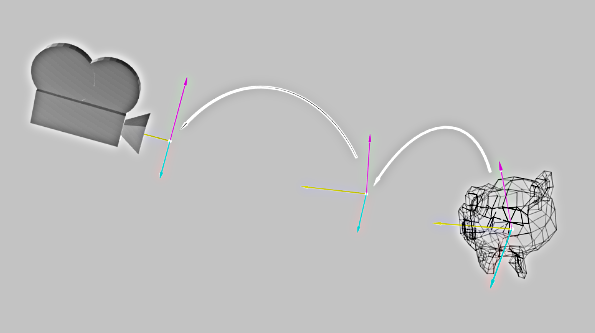
\includegraphics[width=.5\linewidth]{figs/TG_view_matrix_neg.png}
\caption{Efeito da Matriz de Visualização (adaptado de \cite{openGlTutorial}).}
\label{fig:mat_visao}
\end{figure}

A função da matriz de projeção é basicamente fazer com que objetos mais
distantes da câmera pareçam menores, como ocorre no mundo real. No sistema de
coordenadas da câmera dois vértices com um mesmo par de coordenadas $(X_p,Y_p)$
serão renderizados no mesmo local, o que não é sempre verdade. Isto acontece
pois a coordenada $Z_p$ não está sendo levada em conta. Para a profundidade ser
levada em conta e a perspectiva corrigida a matriz de projeção transforma o
espaço de visão da câmera, que inicialmente é um hexaedro irregular, em um cubo
\cite{openGlTutorial}, com isso os objetos são deformados de modo que o que está
mais próximo da câmera pareça maior e o que está mais distante da câmera pareça
menor, tendo-se, por fim, um sistema de coordenadas homogêneas. As Figura
\ref{fig:mat_proj} ilustra o que acontece.

\begin{figure*}[!htb]
   \centering
\begin{tabular}{cc}
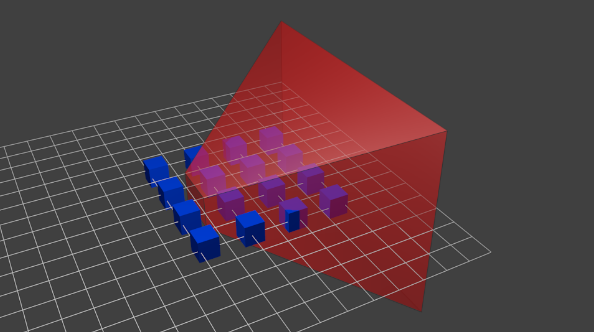
\includegraphics[width=0.4\linewidth]{./figs/TG_projection_matrix_1.png}&
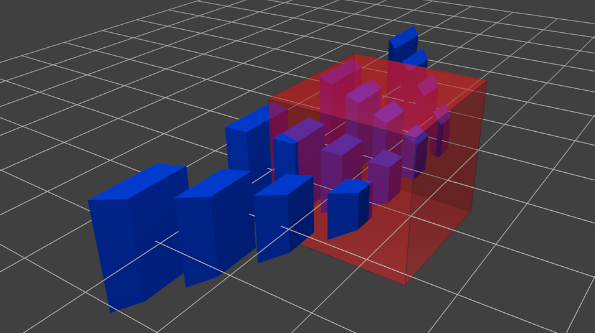
\includegraphics[width=0.4\linewidth]{./figs/TG_projection_matrix_2.png}
\end{tabular}
    \caption{Efeito da Matriz de Projeção (retirado de \cite{openGlTutorial})}
    \label{fig:mat_proj}
\end{figure*}

Um diagrama do efeito dessas três matrizes no sistemas de coordenadas onde se
encontra o objeto pode ser visualizado na Figura \ref{fig:mat_diagrama}.

\begin{figure}[h!]
\centering
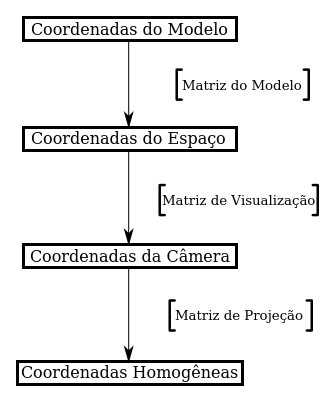
\includegraphics[width=.45\linewidth]{figs/TG_matrices_diagram_pt.png}
\caption{Diagrama do efeito das matrizes (adaptado de \cite{openGlTutorial}).}
\label{fig:mat_diagrama}
\end{figure}

\section{Mistura de Poses}

  Mesmo nas mais simples animações comerciais, um modelo tridimensional
utilizado costuma ser composto por milhares de vértices e polígonos.
Renderizar um rosto expressivo requer definir valores para cada um dos
vértices envolvidos. Adicione ao problema o fato de que um vídeo de poucos
segundos pode exigir centenas de expressões ligeiramente diferente uma da
outra para que o animação seja percebida de forma suave.
    
  Uma das técnicas utilizadas pelos animadores digitais é a Animação
Esqueletal (\textit{Skeletal Animation}) na qual se define um esqueleto
sobre o modelo tridimensional, de forma que movimento de cada ponto sobre o
modelo está atrelado ao movimento de rotação e translação das juntas. O
artista pode então posicionar as juntas em poses chaves do movimento e pedir
para que o computador interpole os pontos intermediários. Comumente, mesmo
depois da interpolação é necessário que o artista retoque manualmente alguns
pontos para que o resultado se torne ainda mais atrativo.
    
    A Figura \ref{fig:rigged-models}, retirada do tutorial em \cite{rigs-tutorial}, mostra a tela do problema \textit{Blender} enquanto o usuário define os \textit{ossos} ou a \textit{armadura} sobre o modelo. Mais tarde, pode-se movimentar os ossos individualmente e a malha do modelo se moverá juntamente.
    
    
\begin{figure*}[!htb]
   \centering
\begin{tabular}{cc}
  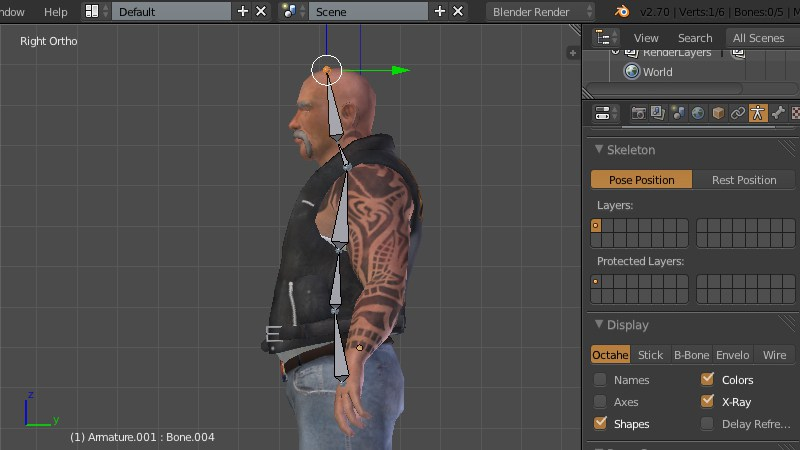
\includegraphics[width=0.4\linewidth]{./figs/blender_armature_image.jpg}
  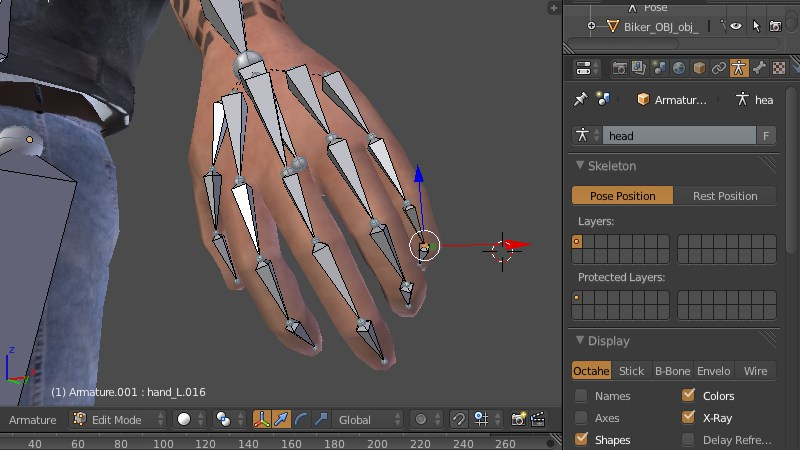
\includegraphics[width=0.4\linewidth]{./figs/blender_armature_image_14.jpg}
\end{tabular}

  \caption{ Tela do programa gratuito de código aberto \textit{Blender} (retirado de \cite{rigs-tutorial}). Cada um dos elementos em cinza é um osso do modelo. O termo utilizado no meio artístico é que se trata de um modelo \textit{rigado}.}

\label{fig:rigged-models} 
\end{figure*}
    
  O uso de \textit{rigged models} é recomendado para animar cenas onde o corpo
inteiro do personagem se mexe. No entanto, é ineficiente para animar
expressões faciais. O problema é que as transformações permitidas pelo modelo
de juntas se limita a transformações rígidas e a forma como os músculos do
rosto se comportam é melhor representada por transformações não rígidas, isto
é, deformações na geometria do corpo.
    
    A técnica de \nomenclature{MP}{\textit{Mistura de Poses}} Mistura de Poses -
MP, do inglês \textit{Blend Shapes} ou \textit{Morph Target}, é uma das
opções comumente empregadas para animar objetos deformáveis como a face
humana. Outros objetos comumente animados com essa técnica são peças de
roupa e pele, uma vez que esses objetos são dificilmente modelados por um
modelo esqueletal \cite{master-thesis-on-blend-shapes}. A técnica consiste
em gerar poses intermediárias como uma combinação linear de poses
pré-definidas. A Figura \ref{fig:blend-shapes-example-input} mostra três
poses utilizadas para a MP mostrada na Figura
\ref{fig:blend-shapes-example-output}.
    
    Em sua versão mais simples, a MP requer que cada um dos modelos
representando as poses chaves tenham a mesma quantidade de vértices. Mais do
que isso, é necessário que se seja capaz de mapear todos os pontos de um
modelo nos pontos de outro. Colocando de outra forma, dá-se um identificador
para cada vértice que compõe a malha do modelo
\cite{tutorial-supremo-on-blend-shapes}.    
    
\FloatBarrier
\begin{figure*}[!htb]
   \centering
  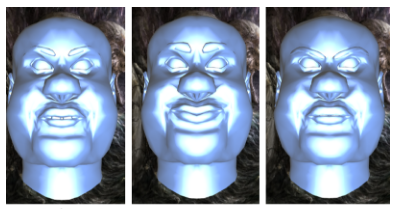
\includegraphics[width=0.7\linewidth]{./figs/inputToBlendShapes.png}

\caption{Três modelos a serem misturados pela técnica de \textit{Blend Shapes}
(retirado de \cite{tutorial-supremo-on-blend-shapes}). Respectivamente da
esquerda para a direita, os modelos representam a pose neutra, a expressão de
felicidade e de raiva. Nota-se a diferença na forma dos lábios e nas sobrancelhas.}

\label{fig:blend-shapes-example-input} 
\end{figure*}

\begin{figure*}[!htb]
   \centering
  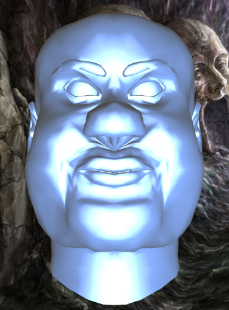
\includegraphics[width=0.6\linewidth]{./figs/outputOfBlendShapes.png}

\caption{Resultado obtido ao combinar 0.5 da pose alegre, 0.3 da pose com raiva e 0.2 da pose neutra (retirado de \cite{tutorial-supremo-on-blend-shapes}).}

\label{fig:blend-shapes-example-output} 
\end{figure*}

% \FloatBarrier
    
    Um modelo M(t) que se deforma no tempo é dado pela tupla de $N$ pontos
    tridimensionais $ ( v_1(t), v_2(t), \ldots,  v_N(t))$. Considere o espaço de
    poses ao longo do tempo $\Omega = \{ M(t), t \in R\}$  e amostre $L$ poses
    distintas $M_i = M(t_i), i = 1 \ldots L$. A MP consiste em construir o
    espaço das poses que podem ser obtidas como uma combinação linear das poses
    amostradas, limitado a fato de que a soma dos coeficientes da combinação
    seja unitária. Além disso, é comum que se defina uma das amostras como a
    pose neutra $M_1$. O peso dessa amostra neutra é escolhido como o negativo
    da soma das outras amostras mais um.
    
    Uma pose $J$ pertencente ao espaço de poses criado deve ser obtido por:    

\begin{equation}
    	J = \sum_{i=1}^L  w_i M_i
        \label{eq:J-mistura}
\end{equation}

Um pouco de manipulação pode deixar mais clara a forma como a mistura de
deformações não rígidas acontece.

\begin{equation}
    	J = w_1 M_1 + w_2 M_2 + \ldots + w_L M_L
\end{equation}

\begin{equation}
    	J = (1-(w_2 + w_3 + \ldots w_L)) M_1 + w_2 M_2 + \ldots + M_\theta + \ldots + w_L M_L
\end{equation}

\begin{equation}
    	J = M_1 + w_1(M_2 - M_1) + \ldots + w_L (M_L - M_1)
\end{equation}

\begin{equation}
    	J = M_1 + \sum_{i = 2}^L w_i \Delta M_i
        \label{eq:blendshapes}
\end{equation}

sendo $\Delta M_i = M_i - M_1$ é a deformação relativa entre $M_i$ e $M_1$. A
última equação deixa claro que as poses obtidas podem ser vistas como a soma de
deformações conhecidas superpostas com a pose neutra. 

Programas de animação utilizam a Equação \ref{eq:blendshapes} da seguinte
maneira: \begin{itemize}

  \item modela-se a pose neutra do seu personagem; 

    \item geram-se expressões chaves a partir da pose neutra apenas pela
      movimentação dos seus vértices;

    \item carrega-se a pose neutra e as demais no framework de mistura de poses
      chaves;

    \item mexendo-se em cursores associados ao peso de cada pose na mistura
      produzem-se  poses intermediárias que são marcadas a pontos no tempo do
      vídeo;

    \item pede-se então que o programa interpole as posições marcadas para que o
      resultado seja suave.

\end{itemize}

A técnica de Animação Esqueletal e a MP são semelhantes no fato em que o artista
configura poses chaves e então o computador completa as lacunas por meio de
interpolação. No entanto, as técnicas produzem resultados de natureza diferente.
Enquanto a primeira pode produzir um braço que tem a junta do cotovelo em
$45^\circ$, a MP produz um rosto que está meio bravo, meio alegre.

Colocando-se em termos bem simples, depois que os modelos para as poses chaves
estão prontos, a técnica de MP recebe um vetor de pesos e produz uma nova pose
como uma média ponderada das poses chaves.

  Programas que realizam a técnica de mistura de poses chaves não são novidade.
  O nosso objetivo é substituir a mão do artista mexendo os cursores de uma
  interface gráfica, por um programa que associa posições do cursor a
  propriedades do vídeo em execução.


\section{Estabilização do movimento}

Devido a ruídos oriundos do processo de captura de imagem e mesmo a
características estatísticas de alguns algoritmos de rastreamento, é comum que o
resultado da detecção oscile em torno do valor correto, mesmo quando a detecção
é feita adequadamente. Em muitas aplicações é desejável que se suavize o
resultado da detecção antes que este seja utilizado para a tomada de decisões. É
com esse objetivo que são utilizadas técnicas de filtragem digital. 

\subsection{Sequências e Sistemas Lineares Invariantes ao Deslocamento}
 
Para a discussão que segue, é dito que uma sequência é uma função $N_0
\rightarrow R$. Isto é, para cada número $n\in \{0,1,2,,\cdots\}$ a sequência
$\chi$ associa o número $\chi(n) \in R$.

Alguns sistemas podem ser descritos por meio de suas respostas a sequências de
entrada. Por exemplo, o sistema $H$  produz a sequência de saída $h(n)$ quando é
submetido a sequência de entrada $\chi(n)$.

Um sistema é dito linear quando vale a seguinte relação:

\begin{equation}
\gamma(n)_{\alpha \chi_1 + \beta \chi_2} = \alpha \gamma_{\chi_1}(n) + \beta \gamma_{\chi_2}(n)
\end{equation}

na qual $\gamma(n)_{\alpha \chi_1 + \beta \chi_2}$ é a resposta do sistema
quando submetido à sequência de entrada $\alpha \chi_1(n) + \beta \chi_2(n)$ e
$\gamma_{\chi_1}(n)$ e $\gamma_{\chi_2}(n)$ são as saídas do sistema quando
submetido a sequências de entrada $\chi_1(n)$ e $\chi_2(x)$ respectivamente. Em
palavras, o sistema é linear quando a sua resposta à combinação linear de dois
sinais é igual à combinação das suas respostas aos dois sinais quando aplicados
independentemente. 

Um sistema é invariante ao deslocamento quando:

\begin{equation}
\gamma_{\chi(n-k)} = \gamma_{\chi(n)}(n - k)
\end{equation}

significando que o comportamento da resposta ao sinal de entrada depende
unicamente do comportamento do sinal de entrada e não do instante em que ele foi
aplicado.

Sistemas Lineares e Invariantes ao Deslocamento (LTI) são úteis pois aproximam
adequadamente o comportamento de muitos sistemas de interesse. Para tais
sistemas vale a seguinte relação: seja $h(n)$ a resposta finita ($h(n) = 0$
$\forall$ $n \geq \mathcal{M}$) de um sistema \nomenclature{LTI}{\textit{Linear
time-invariant}} LTI ao sinal de entrada $\delta(n)$ dado por:

\begin{equation}
    \delta(n)= 
\begin{cases}
    1,& \text{se } n = 0\\
    0,              & \text{caso contrário}
\end{cases}
\end{equation}

o sinal $\gamma(n)$ da resposta do mesmo sistema a um sinal de entrada $\chi(n)$
qualquer será dada por:

\begin{equation}
\gamma(n) = \sum_{k=0} ^{\mathcal{M}-1} h(k)\chi(n-k) = h(n) * \chi(n)
\end{equation}

Com isso, um sistema LTI é muitas vezes representado pela sua resposta $h(n)$ ao
impulso $\delta(n)$.



\subsection{A Transformada Z}

Existem várias maneiras de se representar uma sequência, e a transformada Z pode
ser vista como uma delas. A transformada Z quando aplicada a uma sequência
$\chi:N_t\rightarrow R$ retorna uma função $X_z:C_z\rightarrow X_z$. A
transformada é dada pela Equação \ref{eq:z-trans}:

\begin{equation}
\mathcal{Z} \{ \chi(n) \} = X_z(\mathpzc{z}) = \sum_{i=0}^{\infty} \chi(i)\mathpzc{z}^{-i}
\label{eq:z-trans}
\end{equation}


A informação contida na transformada $\mathpzc{z}$ é, a princípio, a mesma
contida na sequência inicial, mas ao mudar a representação da sequência algumas
de suas características podem ser melhor entendidas. Por exemplo, se $H_z(z) =
\mathcal{Z}\{h(n)\}$ é a transformada da resposta ao impulso do sistema, então é
possível mostrar que a transformada $Y_z(\mathpzc{z})$ da resposta do sistema a
um sinal de transformada $X_z(\mathpzc{z})$ é dada por:

\begin{equation}
Y_z(\mathpzc{z}) = H_z(\mathpzc{z})X_z(\mathpzc{z})
\end{equation}

Outro resultado importante permite recuperar a sequência $\chi(n)$ a partir de
$X_z(\mathpzc{z})$ através da transformada Z inversa:

\begin{equation}
\mathcal{Z}^{-1}\{X_z(\mathpzc{z})\} = \frac{1}{2 \pi} \oint X_z(\mathpzc{z}) \mathpzc{z}^{n-1}dz = \chi(n)
\end{equation}

\subsection{Resposta em Frequência}

A função $X_z(z)$ pode ser avaliada em qualquer ponto $\mathpzc{z} \in C_z$. Em
particular ela pode ser avaliada nos pontos $\mathpzc{z} = e^{j\omega}$ do
círculo unitário. Quando isso é feito, tem-se a transformada de Fourrier em
Tempo Discreto:

\begin{equation}
\label{eq:DFT-transform}
X_d(\omega) = X_z(\mathpzc{z})|_{\mathpzc{z} = e^{j\omega n}} = \sum _{n=0}^{\infty} \chi(n) e^{-j\omega} 
\end{equation}

com transformada inversa:

\begin{equation}
\label{eq:DFT-inverse-transform}
\chi(n) = \frac{1}{2 \pi j} \int _{- \pi}^{\pi} X_d(\omega) e^{j\omega}d\omega
\end{equation}

Este último resultado tem uma interpretação interessante: ele nos diz que uma
sequência x(n) qualquer pode ser obtida como uma combinação de um número
infinito de sequências de uma coleção de sequências exponenciais $\{e^{j\omega},
-\pi \leq \omega \leq \pi \}$. Conhecendo a equação de Euler:

\begin{equation}
\label{eq:euler-equation}
e^{wj} = cos(\omega) + j sen(\omega)
\end{equation}

e com $\omega = 2\pi f_q$, $f_q$ a frequência do sinal, diz-se que uma
\textbf{sequência qualquer $\bm{\chi(n)}$ pode ser escrita como uma combinação
de sequências senoidais primitivas}. A vantagem desta análise é que em muitas
aplicações as componentes senoidais primitivas representam características
físicas do sistema em que se deseja trabalhar. 

Por exemplo, uma sequência obtida por amostragem de um sensor ruidoso é composta
pela justaposição da variável real medida e de diversas interferências. Se em
uma dada aplicação sabe-se que todas as interferências estão associadas a sinais
de alta frequência, é possível se blindar do ruído e recuperar o sinal
verdadeiro apenas filtrando as componentes de alta frequência.

\subsection{Equação de Diferenças}

Uma equação de diferença calcula uma amostra de saída no tempo $n$ baseado em
amostras de entradas passadas e presentes e amostras de saída passadas no
domínio do tempo \cite{classnote-on-difference-equation}. A equação geral para
um sistema causal, linear e invariante no tempo pode ser escrita como:

\begin{equation}
\gamma(n) = \sum_{i=0}^{M_l}b_i \chi(n-i) - \sum_{j=1}^{N_l}a_j \gamma(n-j) 
\end{equation}

Quando a equação de diferenças utiliza amostras de saída passadas (como
$\gamma(n-1)$) no cálculo da amostra de saída presente $\gamma(n)$ dizemos que
há realimentação no sistema. Os coeficientes $b_i$ são chamados de coeficientes
diretos e os $a_j$ são ditos os coeficientes de realimentação
\cite{classnote-on-difference-equation}.

Equações de diferença podem ser utilizadas para implementar filtros digitais.

\subsection{Filtros Digitas}

Um filtro digital é uma forma de ir de um sinal digital para um outro
\cite{classnote-on-intro-to-digital-filters}, podendo ser implementado em
\textit{software}, por meio de uma sub-rotina de computador, como em
\textit{hardware}, por meio de um projeto de circuito integrado. Em aplicações,
filtros digitais são comumente empregados para realçar características do sinal
de interesse ou remover características indesejadas.

Uma forma comum de especificar um filtro digital é por meio da resposta em
frequência. A Figura \ref{fig:filtro-passa-baixas-ideal-freq} mostra a
especificação de um filtro passa baixas ideal. Nesse tipo de filtro, é desejado
remover do sinal de entrada qualquer componente de frequência $\omega >
\omega_c$, na qual $\omega_c$ é a frequência de corte do filtro (em
radianos/segundo).

\subsection{Filtros Digitais de Resposta Finita ao Impulso}

Um filtro digital é dito de \nomenclature{FIR}{\textit{Finite Impulse Response}}
Resposta Finita ao Impulso, do inglês \textit{Finite Impulse Response} (FIR), é
aquele cuja resposta ao impulso tem comprimento finito. Seja $h(n)$ a resposta
do filtro ao impulso $\delta(n)$, o filtro é FIR se $\exists \mathcal{M} \geq 0$
tal que $h(n) = 0$ para todo $n \geq \mathcal{M}$.

Um resultado útil da teoria de Processamento de Sinais Digitais é que um filtro
FIR pode ser implementado por uma equação de diferenças sem realimentação, ou
seja, uma equação da forma:

\begin{equation}
    \gamma(n) = 	\sum_{i=0}^{\mathcal{M}} b_i \chi(n-i)
\end{equation}

Filtros com a forma acima são desejáveis pois são mais facilmente
implementáveis.

\subsection{Projeto de Filtro Passa-Baixa pela Técnica de Janela}

O princípio por trás dessa técnica é se aproximar do filtro passa-baixas ideal,
mostrado na Figura \ref{fig:filtro-passa-baixas-ideal-freq}. A Equação
\ref{eq:DFT-inverse-transform} permite calcular a resposta ao impulso $h(n)$ que
produziria tal filtro ideal.

\begin{figure}[!htb]
  \centering
  \begin{subfigure}[]{\label{fig:filter3}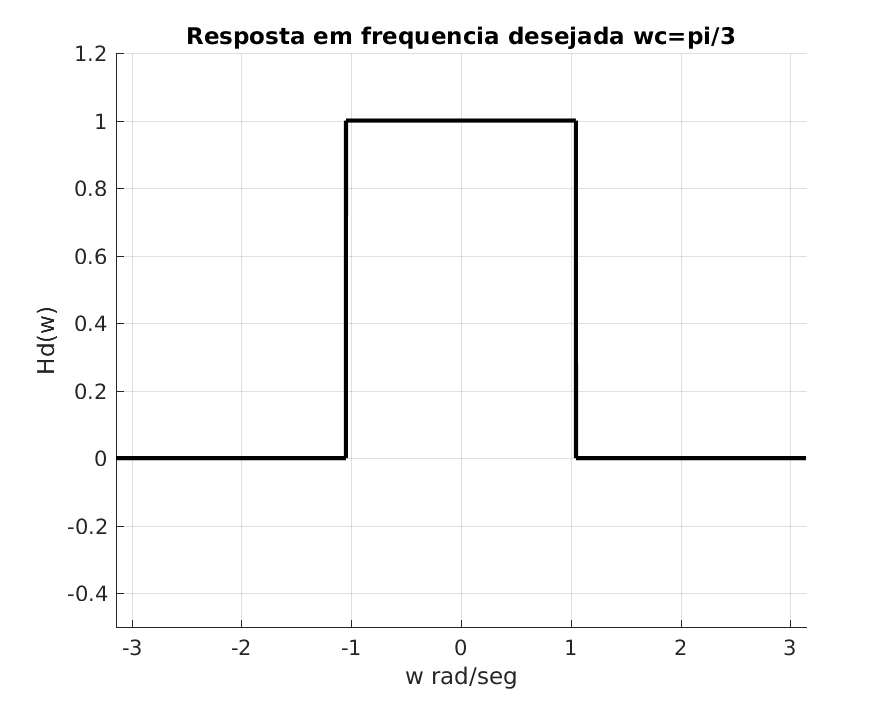
\includegraphics[width=0.4\textwidth]{./figs/idealLowPassFilterResponse.png}}
  \end{subfigure}   
  \begin{subfigure}[]{\label{fig:filter4}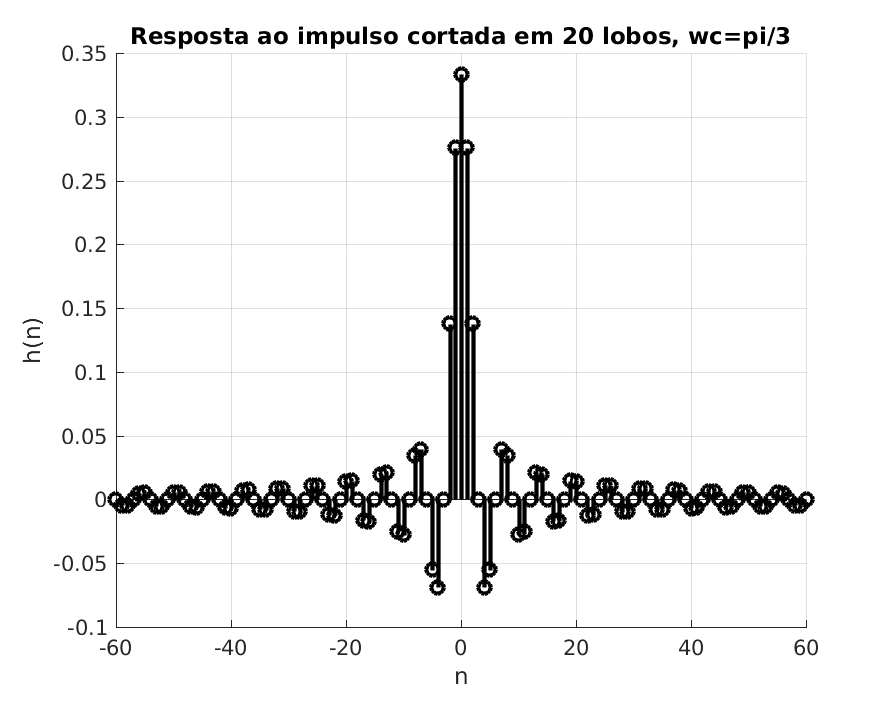
\includegraphics[width=0.4\textwidth]{./figs/infiniteIdealResponse.png}}
  \end{subfigure}

  \caption{Em (a) é observada a resposta ao impulso em frequência ideal de um
    filtro passa-baixas. A frequência de corte projetada é $\omega_c=\frac{\pi}{3}$
    rad/segundos. Em (b) são observados alguns pontos de $h(n)$. Na realidade a sequência é infinita para ambos os lados do eixo.  }

  \label{fig:filtro-passa-baixas-ideal-freq}
\end{figure}

Pode ser observado que além da resposta ser infinita, ela é não causal pois
possui termos não nulos para $n < 0$. Ou seja, o sistema precisaria começar a
responder antes mesmo que a entrada impulso fosse aplicada. Fica claro que a
realização de tal filtro é impossível. Notando que a forma de onda de $h(n)$ é
composta por lobos positivos e negativos, a técnica de janela busca aproximar o
filtro ideal ao limitar $h(n)$ a um número finito de pontos não nulos, de forma
a manter um número inteiro de lobos simétricos. Além disso, $h(n)$ precisa ser
deslocado para a direita caso o objetivo seja um filtro fisicamente realizável. 

A Figura \ref{fig:filtro-passa-baixas-3-lobos} mostra o filtro e a resposta em
frequência obtidos caso a resposta ideal seja cortada com o lobo central e mais
dois lobos simétricos.  A Figura \ref{fig:filtro-passa-baixas-1-lobo} mostra o
filtro e a resposta em frequência obtidos caso mantenha-se somente o lobo
central.  Nota-se que no primeiro caso são necessários 18 valores, enquanto no
segundo apenas 6. Por outro lado, a resposta em frequência no primeiro caso se
aproxima melhor do filtro passa-baixas ideal. Nota-se que há um compromisso que
precisa ser feito entre a qualidade do filtro e a quantidade de memória e
processamento necessários para implementar o filtro.

Para efeito de comparação, a Figura \ref{fig:filtro-passa-baixas-mais-curto}
mostra o mesmo projeto aplicado para a frequência de corte
$\omega_c=\frac{\pi}{10}$. Nota-se que uma frequência de corte mais baixa requer
uma quantidade de pontos não nulos no filtro maior que aquela vista na Figura
\ref{fig:filtro-passa-baixas-3-lobos}.

\begin{figure}[!htb]
  \centering
  \begin{subfigure}[]{\label{fig:filter1}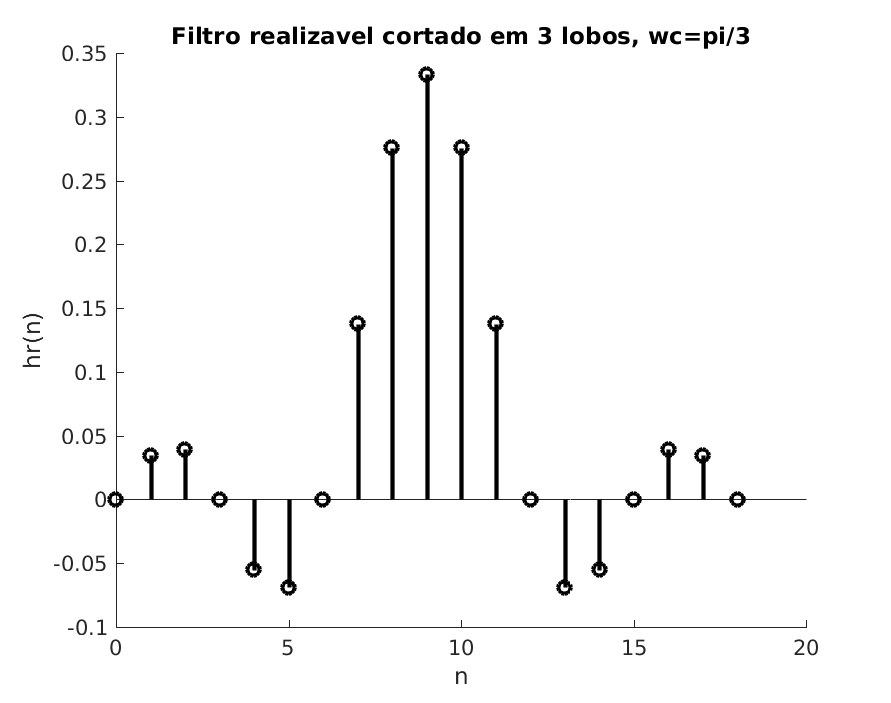
\includegraphics[width=0.4\textwidth]{./figs/realizableFilter3L3.png}}
  \end{subfigure}   
  \begin{subfigure}[]{\label{fig:filter2}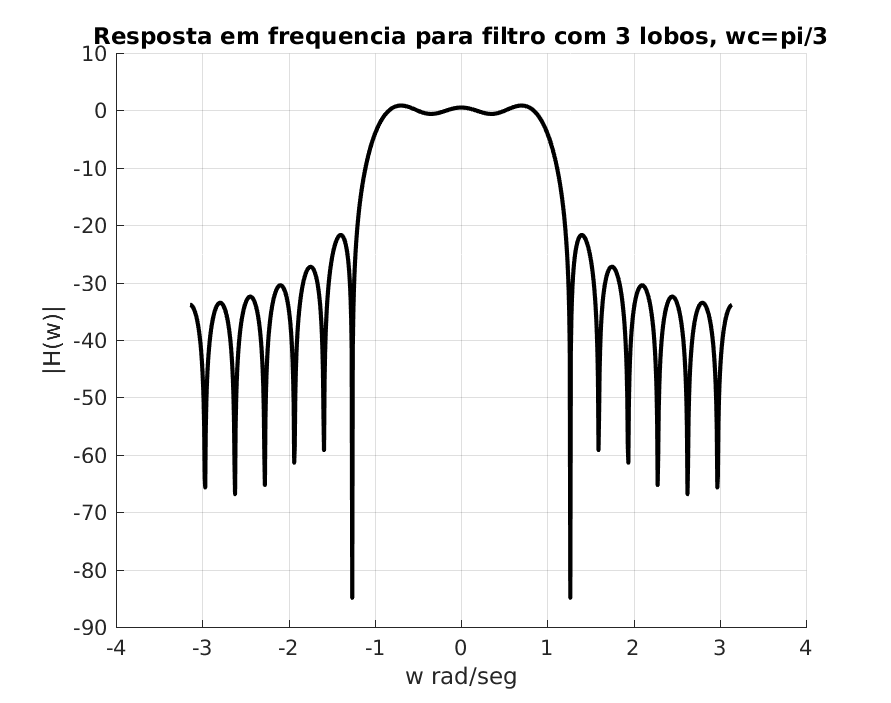
\includegraphics[width=0.4\textwidth]{./figs/filterResponse3L3.png}}
  \end{subfigure}

  \caption{Em (a) é observada a resposta ao impulso do filtro realizável obtido
    cortando-se o lobo principal mais dois lobos para cada lado da resposta
    ideal.  Note que o eixo horizontal foi transladado para permitir uma
    resposta realizável. Em (b) é observada a resposta em frequência obtida com
    esse filtro.  Nota-se que o eixo vertical é mostrado em decibéis.}

  \label{fig:filtro-passa-baixas-3-lobos}
\end{figure}

\begin{figure}[!htb]
  \centering
  \begin{subfigure}[]{\label{fig:filter3}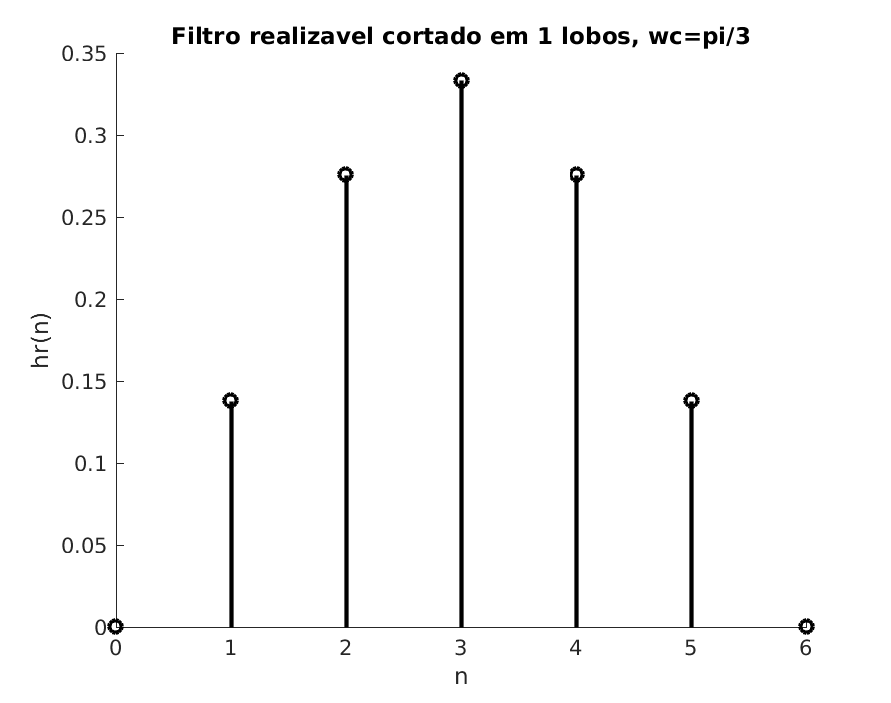
\includegraphics[width=0.4\textwidth]{./figs/realizableFilter1L3.png}}
  \end{subfigure}   
  \begin{subfigure}[]{\label{fig:filter4}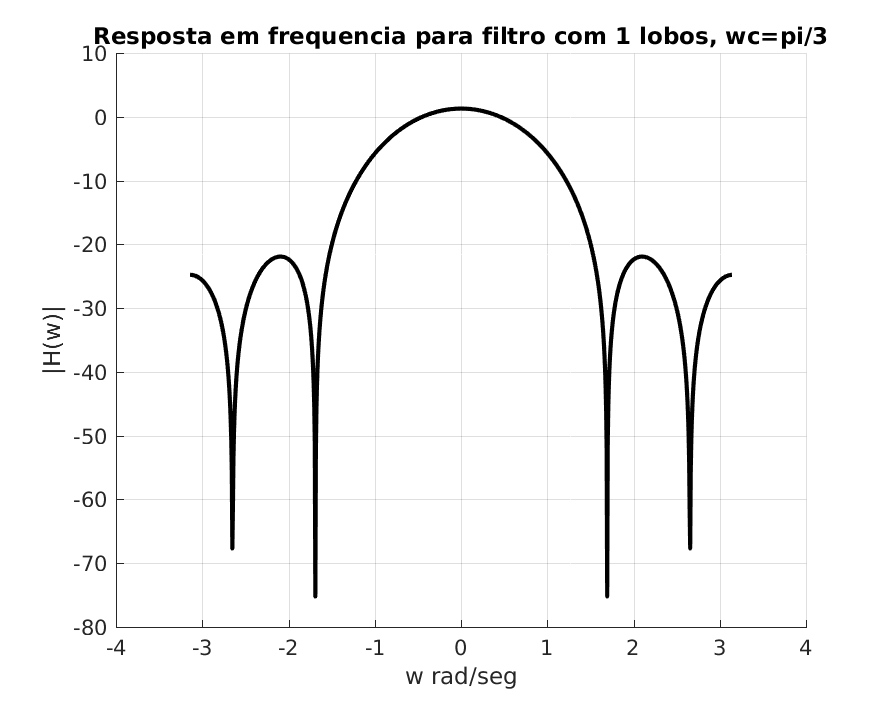
\includegraphics[width=0.4\textwidth]{./figs/filterResponse1L3.png}}
  \end{subfigure}

  \caption{Em (a) é observada a resposta ao impulso do filtro realizável obtido
  cortando-se o lobo principal somente. Em (b) é observada a resposta em
frequência obtida com esse filtro.}

  \label{fig:filtro-passa-baixas-1-lobo}
\end{figure}

\begin{figure}[!htb]
  \centering
  \begin{subfigure}[]{\label{fig:filter3}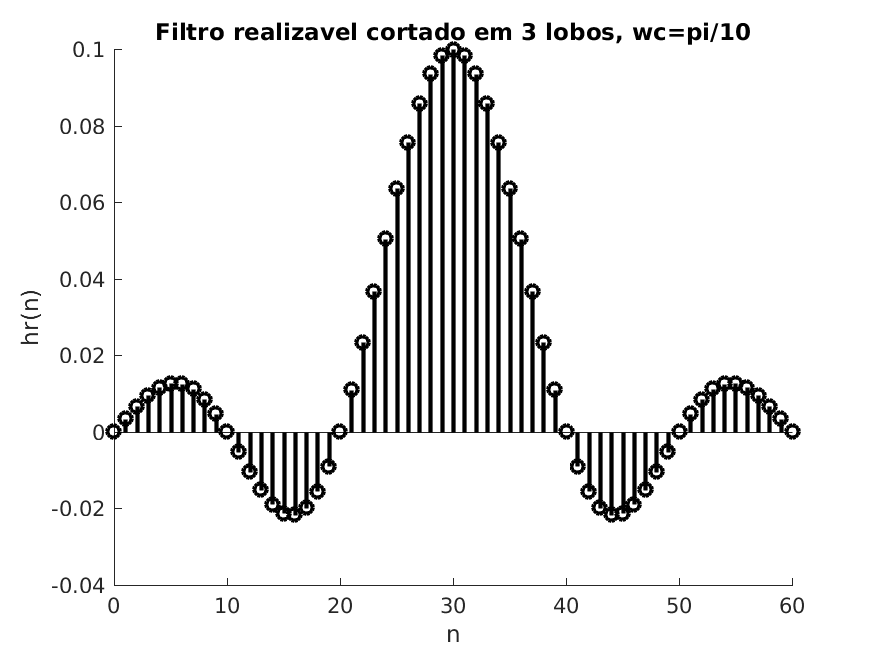
\includegraphics[width=0.4\textwidth]{./figs/realizableFilter3L10.png}}
  \end{subfigure}   
  \begin{subfigure}[]{\label{fig:filter4}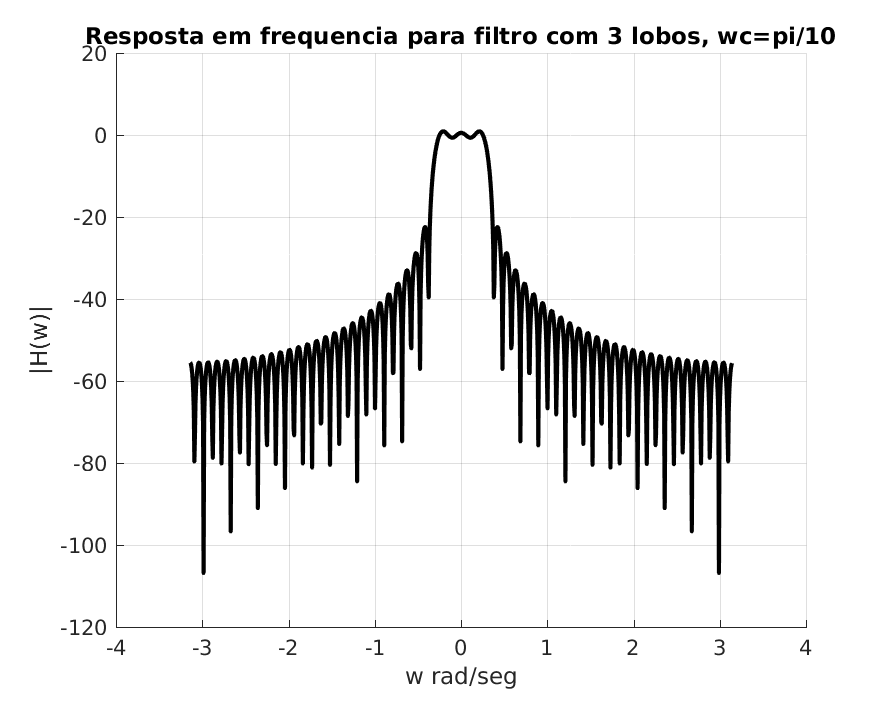
\includegraphics[width=0.4\textwidth]{./figs/filterResponse3L10.png}}
  \end{subfigure}

  \caption{Filtro projetado com 3 lobos e frequência de corte
  $w_c=\frac{\pi}{10}$.}

  \label{fig:filtro-passa-baixas-mais-curto}
\end{figure}



\chapter{Metodologia}

Este capítulo descreve a sequência de passos utilizada para extrair movimento
facial a partir de um par de imagens e transferi-lo para um modelo
tridimensional. O objetivo do sistema de animação computacional de baixo 
custo proposto é a transferência de movimento
da imagem para o modelo. Portanto a qualidade do resultado final deve ser
analisada através da comparação entre o movimento esperado e aquele efetivamente
gerado. Este trabalho não propõe uma metodologia formal para a avaliação da
qualidade final, essa avaliação é feita de forma qualitativa pela observação dos
resultados. No entanto, métricas consideradas mais quantitativas podem ser
definidas para as etapas intermediárias da aplicação e alguns experimentos são
propostos com o objetivo de avaliá-las. Este capítulo é dividido em duas partes:
a primeira descreve as etapas da aplicação proposta e a segunda descreve os
experimentos de validação dessas etapas.

\section{Etapas de Desenvolvimento}

A Figura \ref{fig:metodologia} apresenta um diagrama que ilustra as etapas da
implementação do método bem como relaciona todas as técnicas utilizadas. As
etapas apresentadas representam  o caminho dos dados dentro de cada iteração do
programa em execução.  Como sugerido pelo diagrama, as etapas são as seguintes:
Posicionamento das Câmeras para Captura das Imagens de Entrada, Rastreamento de
Pontos do Rosto, Estimação da Profundidade, Atualização dos Pesos de Mistura -
Razão de Distância, Filtros e Mistura de Poses. 

\begin{figure}
\centering
\includegraphics[width=0.9\linewidth]{figs/TG-metodologia-correta-2.png}

\caption{Diagrama completo para a animação de cada \textit{frame}. As setas
verticais representam o fluxo entre as técnicas dentro de cada iteração do
programa. As setas horizontais indicam dados provenientes de uma etapa de
calibração do sistema.}

\label{fig:metodologia}
\end{figure}



\subsection{Posicionamento das Câmeras para Captura das Imagens de Entrada}


A estrutura utilizada neste trabalho para captura de vídeo consiste na fixação
de duas \textit{webcams} comuns posicionadas paralelamente sobre uma plataforma
de madeira. A Figura \ref{fig:setupCameras} mostra a fixação do par de câmeras
utilizado, sendo `$b = 18cm$'  a distância entre os centros das câmeras e `$a =
2 cm$' a distância entre o centro de captura da câmera e a aresta do suporte.
Este parâmetro $a$ deve ser conhecido pois durante os experimentos é necessário
medir a distância do alvo ao centro das câmeras e isso é mais facilmente feito
tomando-se a distância do alvo ao suporte e utilizando o parâmetro $a$ para
recuperar a medida necessária. O parâmetro $b$ é utilizado durante a etapa de
estimação de profundidade e é equivalente ao que foi chamado de
\textit{baseline} na Figura \ref{fig:disp_cameras}. A câmera de índice 1 é
aquela que fica à direita do usuário quando este encontra-se de frente para a
montagem na Figura \ref{fig:setupCameras} e a de índice 2 é aquela que se
encontra à esquerda. Ao relacionar os pontos da câmera aos termos da Equação
\ref{eq:3d_Zequation}, chama-se o ponto alvo projetado no plano da imagem da
câmera 1 de $u$ e o ponto alvo projetado no plano da imagem da câmera 2 de $u'$.
Além disso, ao conectar as câmeras às entradas USB do computador que roda a
aplicação, deve-se conectar primeiramente a câmera 1 e em seguida a câmera 2.
Isso deve ser feito para que o programa localize corretamente as câmeras,
definindo qual imagem de entrada é proveniente da câmera da direita e qual é
proveniente da câmera da esquerda. 


\begin{figure}[!htb]
\centering
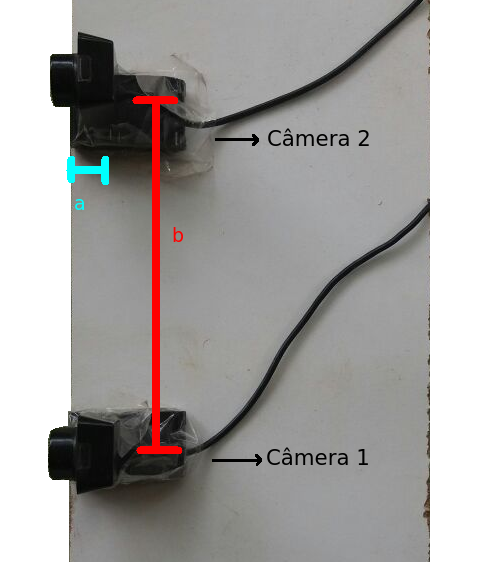
\includegraphics[width=0.7\textwidth]{figs/setupExperimento-marcado_edit-2.png}
\caption{Fixação das câmeras. Estrutura utilizada neste trabalho para a captura das imagens de entrada.}
\label{fig:setupCameras}
\end{figure}



\subsection{Rastreamento de Pontos do Rosto}

O rastreamento de pontos do rosto é a segunda etapa do processo iterativo de
animação implementado neste trabalho. Como pode ser visto na Figura
\ref{fig:metodologia}, em cada iteração do programa em execução as duas imagens
de entrada passam por esse processo separadamente.

Para fins de rastreamento de pontos do rosto, utiliza-se a
\nomenclature{SDK}{\textit{Software Development Kit}} \textit{Software
Development Kit} (SDK) \textit{CSIRO Face Analysis} \cite{cox2013csiro}
desenvolvida utilizando a biblioteca \nomenclature{OpenCV}{\textit{Open Source
Computer Vision}} \textit{Open Source Computer Vision} (OpenCV) para
representação e manipulação de imagens e vídeos. Para que ocorra o rastreamento
de pontos exige-se que a imagem de entrada esteja no formato \textit{grayscale}
(níveis de cinza). Caso não esteja, deve-se primeiramente transformar a imagem
de entrada para este formato. 

Para rastrear pontos da face a SDK implementa a técnica RMLS introduzida na
fundamentação. O Algoritmo \ref{alg:rlms} descreve de forma simplificada os
passos tomados para se obter o rastreamento \cite{saragih2011deformable}. A
variável $\mathbf{p}$ no algoritmo representa os parâmetros do PDM e com ela
calculada pode-se obter a posição dos pontos de interesse através da Equação
\ref{eq:PDM-equation}. Um detalhamento da técnica pode ser encontrado em
\cite{saragih2011deformable}.

\begin{algorithm}[!htb]
\caption{RLMS (\textit{Regularized landmark mean-shift})}\label{alg:rlms}
\begin{algorithmic}[1]
\Require{$\mathcal{I}$ e $\mathbf{p}$} \Comment{$\mathcal{I}$ sendo a imagem e $\textbf{p}$ como definido na Equação \ref{eq:alg1}}
\State Computar respostas [Equações \ref{eq:alg1}]
   \While{nao{\_}convergiu(\textbf{p})}
   \State Linearizar o modelo de forma [Equação \ref{eq:alg2}]
   \State Computar os vetores do deslocamento da média [Equação \ref{eq:alg3}]
   \State Computar a atualização dos parâmetros PDM [Equação \ref{eq:alg4}]
   \State Atualizar parâmetros: $\textbf{p} \leftarrow \textbf{p} + \Delta\textbf{p}$
   \EndWhile
   \State \textbf{return} $\textbf{p}$
\end{algorithmic}
\end{algorithm}





O resultado do rastreamento é um arranjo de 66 pontos contendo os valores das
coordenadas $(x,y)$ na imagem de cada ponto chave. A SDK ordena os pontos
retornados de forma que cada ponto chave esteja sempre em uma mesma posição do
arranjo. Os pontos rastreados e a numeração associada a cada um deles são
mostrados na  Figura \ref{fig:tracked-facial-points}. 

\begin{figure*}
\centering
\begin{tabular}{cc}
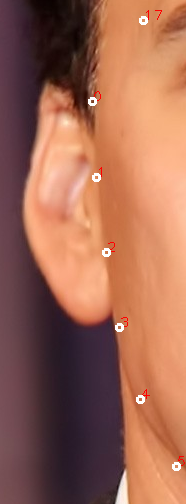
\includegraphics[width=0.4\linewidth, height=5cm]{figs/nick-marked-l-ear.png} &
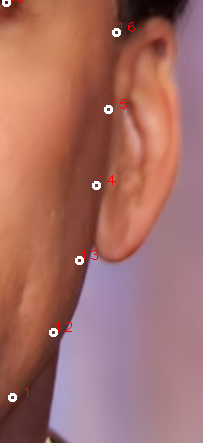
\includegraphics[width=0.4\linewidth, height=5cm]{figs/nick-marked-r-ear.png} \\
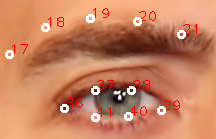
\includegraphics[width=0.4\linewidth, height=5cm]{figs/nick-marked-l-eye.png} &
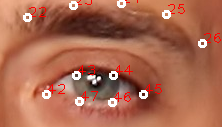
\includegraphics[width=0.4\linewidth, height=5cm]{figs/nick-marked-r-eye.png} \\
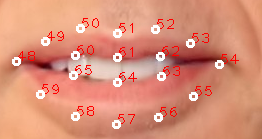
\includegraphics[width=0.4\linewidth, height=5cm]{figs/nick-marked-mouth.png} &
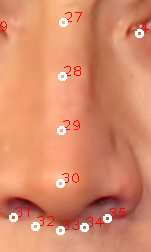
\includegraphics[width=0.4\linewidth, height=5cm]{figs/nick-marked-nose.png} \\
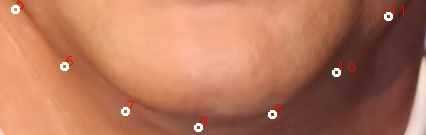
\includegraphics[width=0.4\linewidth, height=5cm]{figs/nick-marked-queixo.png} &
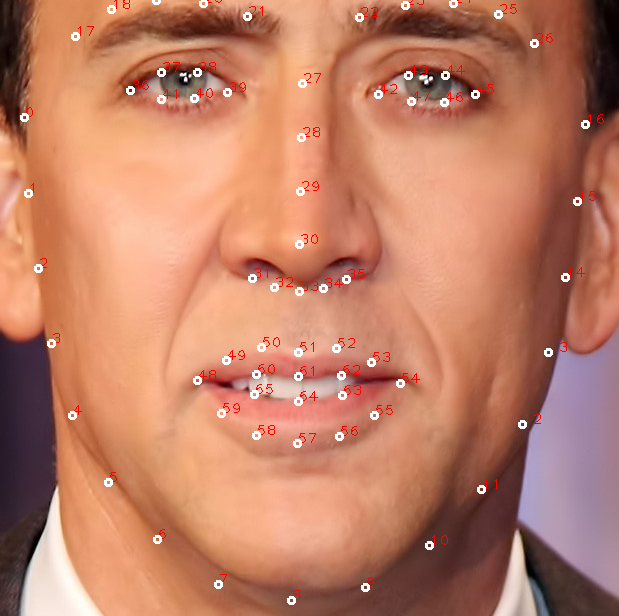
\includegraphics[width=0.4\linewidth, height=5cm]{figs/nick-marked.png}
\end{tabular}
\caption{Pontos retornados pelo rastreamento facial e a numeração associada a cada ponto. A imagem sobre a qual se realiza o rastreamento (retirado de \cite{nicolas}).}
\label{fig:tracked-facial-points}
\end{figure*}


Além dos pontos retornados, um valor entre zero e dez representando a qualidade
da detecção é fornecido ao final de cada rastreamento. Esse valor serve para
avaliar se a detecção do quadro atual deve ser utilizada, para assim atualizar a
malha tridimensional: caso o valor da qualidade de detecção seja zero em uma
iteração, o modelo não é atualizado. Além disso, uma qualidade de zero indica
que o rastreamento perdeu completamente os pontos de interesse e é necessário
reinicializar o rastreador para que a detecção tenha chance de ser realizada com
sucesso na próxima iteração.

Além disso, como o rastreamento é aplicado independentemente a cada uma das
imagens de entrada, é importante que se mantenham dois rastreadores
inicializados e atualizados independentemente. Isso deve ser feito pois a SDK
reutiliza informações de estados anteriores para acelerar o rastreamento no
quadro atual e não se deve misturar o estado do rastreamento na imagem esquerda
com o estado do rastreamento na imagem direita. 

A saída desta etapa como um todo consiste de dois conjuntos de 66 pontos
bidimensionais enumerados, uma para cada imagem, bem como dois parâmetros que
representam a qualidade do rastreamento feito em cada imagem. 

\subsection{Estimação da Profundidade}

Como ficará colocado em mais detalhes nas próxima seções, esta aplicação utiliza
a distância entre pontos do rosto para interpretar a posição que deve ser
transferida para o modelo. Sem a estimação de profundidade, a distância entre
dois pontos do rosto diminuiria a medida que o usuário se afastasse do par de
câmeras e colocaria sobre o usuário a responsabilidade de realizar gravações
sempre a uma mesma distância. Além disso, uma leve movimentação despercebida
durante as gravações poderia ser erroneamente interpretada pelo programa, já que
decisões são tomadas a partir do movimento entre os pontos e um afastamento do
usuário causaria uma redução em todas as distâncias.  A estimação da
profundidade permite que medidas retiradas da imagem sejam independentes da
distância em que o usuário se encontra das câmeras, o que garante maior
flexibilidade de uso e uma maior estabilidade na animação. Com a estimação da
profundidade é possível aproximar os valores $X$, $Y$ e $Z$ dos pontos de
interesse no sistema de coordenadas do mundo. Por exemplo, a distância entre os
dois olhos do usuário deve ser sempre a mesma e pode ser medida em centímetros e
não mais em pixeis.

A estimação da profundidade é feita utilizando-se os dois conjuntos de pontos
fornecidos pela etapa de rastreamento. Um exemplo de um par de imagens de
entrada onde o rastreamento foi aplicado e os pontos marcados pode ser observado
na Figura \ref{fig:input_images}. As imagens tiradas em uma mesma iteração do
programa por câmeras diferentes mostram o usuário em  uma posição ligeiramente
deslocada em relação a outra, e é justamente essa diferença horizontal que é
utilizada para estimar a profundidade. Além disso, uma vez estimada a
profundidade, pode-se corrigir a posição horizontal dos pontos de
interesse\footnote{Vale lembrar que assume-se que os centros de captura das
câmeras estão alinhados verticalmente e, portanto, não espera-se diferença entre
as coordenadas Y de um mesmo ponto do rosto nas duas imagens.}.

\begin{figure}[!htb]
  \centering
  \begin{subfigure}[]{\label{fig:filter3}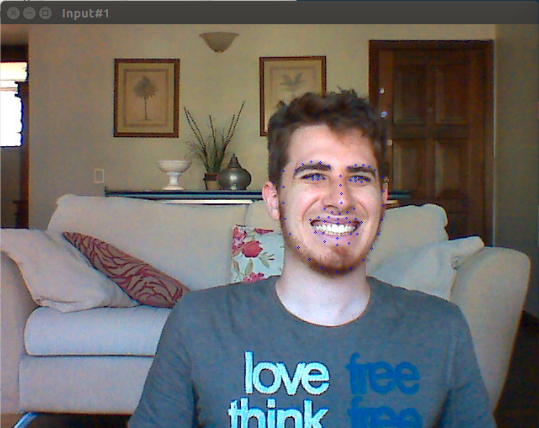
\includegraphics[width=0.45\textwidth]{./figs/TG_input_image1.png}}
  \end{subfigure}   
  \begin{subfigure}[]{\label{fig:filter4}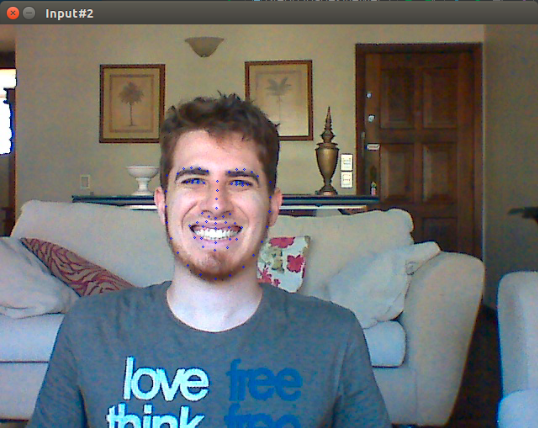
\includegraphics[width=0.45\textwidth]{./figs/TG_input_image2.png}}
  \end{subfigure}

  \caption{ Imagens extraídas da câmera 1 (a) e da câmera 2 (b) em uma mesma
  iteração do programa em execução. Ao comparar as duas imagens, nota-se que o
usuário aparece deslocado horizontalmente em uma imagem quando comparado a
outra. Os pontos de interesse foram rastreados e marcados com círculos azuis.}

\label{fig:input_images}
\end{figure}

Como o cojunto de pontos rastreados é sempre ordenado da mesma maneira, é fácil
localizar o mesmo ponto do rosto em cada uma das imagens: basta tomar os mesmos
índices em cada um dos vetores retornados pela etapa de rastreamento. Esse
mapeamento de pontos é utilizado para estimar a posição no mundo de cada um dos
pontos rastreados, isso é feito através de uma semelhança de triângulos, como
foi resumido na Equação \ref{eq:3d_Zequation} apresentada na fundamentação
teórica.

Vale notar que para a aplicação da Equação \ref{eq:3d_Zequation} deve-se
anteriormente conhecer a distância focal de cada uma das câmeras, o que pode ser
obtido pela utilização da ferramenta \textit{Calibration Toolbox}, uma extensão
disponível para Matlab. O processo de calibração de uma câmera por meio dessa
ferramenta consiste na captura de vinte imagens de um tabuleiro de xadrez em
diferentes posições. Após a marcação manual das extremidades desse tabuleiro, o
algoritmo de calibração realiza um processo de detecção em cada uma das imagens
de um conjunto de pontos conhecidos - as quinas de cada um dos quadrados do
tabuleiro de xadrez . O mapeamento desses pontos em cada uma das imagens em
conjunto com o conhecimento do tamanho real de cada uma das casas do tabuleiro
permite determinar a matriz de calibração da câmera, que inclui, dentre outros
valores, os parâmetros intrínsecos da câmera. Um exemplo do conjunto de imagens
utilizado durante a etapa de calibração pode ser observado na Figura
\ref{fig:calib_imagens}.  A calibração\footnote{O termo `calibração' aqui
significa a realização de um processo que estima os parâmetros de interesse.
Nenhuma modificação é aplicada sobre os sensores em si.} é feita após o processo
de fixação das câmeras e os resultados guardados para utilização enquanto os
resultados da estimação de profundidade se mostrarem satisfatórios. Vale notar
que choques ocasionais aplicados a montagem podem alterar os parâmetros das
câmeras e requerer uma recalibração destes. 

\begin{figure}[h!]
\centering
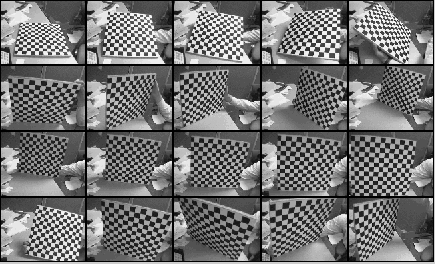
\includegraphics[width=.6\linewidth]{figs/TG_calib_images.png}
\caption{Exemplo de imagens utilizadas em uma calibração (retirado de \cite{bouguetML}).}
\label{fig:calib_imagens}
\end{figure}

A matriz $KK$ dos parâmetros intrínsecos da câmera obtida por uma calibração
feita utilizando a \textit{Calibration Toolbox for Matlab} é mostrada na Equação
\ref{eq:calib_matIntrinseca}.

\begin{align}
KK =
\left[\begin{array}{ccc}
f_c(1) & alpha_c*f_c(1) & cc(1)\\
0 & f_c(2) & cc(2)\\
0 & 0 & 1
\end{array}\right]
\label{eq:calib_matIntrinseca}
\end{align}

Onde $f_c(1)$ e $f_c(2)$ são as distâncias focais descritas em unidades de
pixeis horizontais e verticais, o coeficiente $alpha_c$ é o ângulo entre os
eixos de coordenadas $x$ e $y$ e os valores de $cc(1)$ e $cc(2)$ representam as
coordenadas $x$ e $y$ do ponto principal da câmera.

Caso seja considerado um pixel quadrado, ou seja, $alpha_c = 0$ e $f_c(1) =
f_c(2)$, essa matriz intrínseca será igual a matriz definida na Equação
\ref{eq:3d_matIntrinseca}.

De posse de todas as variáveis é então possível estimar o valor $Z$ de um ponto
no mundo e com isso estimar também os valores $X$ e $Y$ deste mesmo ponto. O
cálculo dos valores $X$ e $Y$ é feito por meio das Equações \ref{eq:3d_realX1} e
\ref{eq:3d_realX2} e das Equações \ref{eq:3d_realY1} e \ref{eq:3d_realY2},
respectivamente.    

Sumarizando, a etapa de estimação de profundidade utiliza os \textbf{dois}
conjuntos de pontos \textbf{bidimensionais} provenientes da etapa de
rastreamento para produzir \textbf{um} conjunto de sessenta e seis pontos
\textbf{tridimensionais} contendo cada um os valores $(X,Y,Z)$ referentes às
coordenadas de cada ponto rastreado no sistema de coordenadas do mundo. Além de
adicionar a componente de profundidade, esta etapa retorna os valores em
centímetros das componentes dos elementos do conjunto produzido.

\subsection{Atualização dos Pesos de Mistura - Razão de Distância}

Até este ponto a aplicação obteve uma estimação para as coordenadas espaciais de
um conjunto de pontos de interesse da face humana. Passa-se agora para a etapa
de extração de informação de pose a partir desse conjunto de pontos. Como será
detalhado na próxima seção, isso é feito por meio da técnica de mistura de poses
que requer como entrada um vetor de pesos. O objetivo desta etapa pode ser posto
como inferir um vetor de pesos que adequadamente produzirá uma mistura de poses
cujo resultado se assemelha com a expressão facial na imagem de entrada.

Define-se cada uma das componentes do vetor de peso independentemente como uma
\textbf{razão de distâncias} entre dois pontos do conjunto de pontos fornecidos
pela etapa de rastreamento. A razão é tomada entre a distância entre os pontos
medida no quadro considerado e a distância entre esses mesmos pontos em quadros
de uma etapa de calibração. Como o interesse é a variação percentual, o que é
medido é de fato a fração que a distância atual se encontra entre a distância
máxima e a mínima medida para o par de pontos.

Seja o peso $w_i^j$ associado com o par de pontos $(\bm{p_1^i}, \bm{p_2^i})$ no
quadro j e seja $d_i^j = |\bm{p_1^i} - \bm{p_2^i}|$ a distância medida entre
esse par de pontos nesse quadro, o peso da i-ésima pose é dado por:

\begin{equation}
	w_i^j = \frac{|d_i^j - d_i^{\text{min}}|}{|d_i^{\text{max}} - d_i^{\text{min}}|}
   \label{eq:pesos1}
\end{equation}

onde $d_i^{\text{min}}$ e $d_i^{\text{max}}$ são as distâncias mínimas e máximas
respectivamente para o par de pontos associado ao peso $w_i$ obtidas em uma
etapa de calibração. 

A Equação \ref{eq:pesos1} descreve poses onde um aumento na razão de distância
significa um aumento no peso da pose associada. No caso de poses onde o oposto
deve acontecer, ou seja, uma diminuição da razão de distância significa um
aumento do peso da pose associada, a equação de peso é dada por: 

\begin{equation}
	w_i^j = 1 - \frac{|d_i^j - d_i^{\text{min}}|}{|d_i^{\text{max}} - d_i^{\text{min}}|}
    \label{eq:pesos2}
\end{equation}

A Equação \ref{eq:pesos2} é utilizada, por exemplo, para o peso associado a pose
que fecha um dos olhos. Nesta pose, quanto maior o peso associado, mais fechado
o olho se encontra. Por outro lado, quando mais fechado o olho, menor a
distância vertical entre pontos ao longo das pálpebras de cima e de baixo desse
olho.

Nota-se que as equações apresentadas descrevem cada peso como um valor entre 0 e
1. No entanto, o modelo de poses utilizado requer que a soma dos pesos resulte
em 1. Para garantir essa condição, o peso da pose neutra é escolhido como:

\begin{equation}
	w_{\text{neutra}}^j = 1 - \sum_{i} w_i^j
    \label{eq:pesos3}
\end{equation}

onde i varia no intervalo de índices das poses de ação (as poses excluindo a
pose neutra).

Resumindo, para cada pose disponível na mistura de poses escolhe-se dois pontos
do conjunto de pontos da etapa de estimação de profundidade e define-se o peso
da pose associada a partir da comparação entre a  distância entre esses dois
pontos no quadro atual e a a distância entre esses dois pontos em quadros de uma
etapa de calibração. Os quadros da etapa de calibração são dois: um
correspondente a 0\% da pose e outro correspondendo a 100\% da aplicação da
pose.

O par de pontos utilizados para cada uma das poses disponíveis para mistura são
listados na Tabela \ref{tab:sensors}. Para cada ponto apresenta-se o índice
correspondente no vetor de 66 pontos da etapa de rastreamento, bem como uma
descrição de sua localização no rosto. O mapeamento entre o índice de pose e a
sua descrição é apresentado na Tabela \ref{tab:poses-descr}. 

\begin{table}[!htb]
\centering
\begin{tabular}{|l|l|l|l|l|}
\hline
k &  $i_k$ & descrição de $p_{i_k}$ & $j_k$ & descrição de $p_{j_k}$ \\ \hline
1 &  54 & canto esquerdo da boca & 48  & canto direito da boca \\ \hline
2 & 24 & centro da sobrancelha esquerda & 42 & canto direito do olho esquerdo \\ \hline
3 & 19 & centro da sobrancelha direita & 39 & canto esquerdo do olho direito \\ 	\hline
4 &  43 & canto superior do olho esquerdo & 47 & canto inferior do olho esquerdo \\ \hline
5 &  37 & canto superior do olho direito & 41 & canto inferior do olho direito \\ \hline
6 &  61 & centro inferior do lábio superior& 64 & centro superior do lábio inferior \\ \hline
\end{tabular}
\caption{Pares de pontos utilizados para razão de distâncias. O peso $w_k$ está associado com o par $(p_{i_k},p_{j_k})$. Os índices dos pontos podem ser comparados com os índices da Figura \ref{fig:tracked-facial-points}}
\label{tab:sensors}
\end{table}

\begin{table}[!htb]
\centering
\begin{tabular}{|l|l|}
\hline
k & pose k  \\ \hline
1 & sorrir  \\ \hline
2 & levantar da sobrancelha esquerda\\ \hline
3 & levantar da sobrancelha direita \\ 	\hline
4 & fechar do olho esquerdo  \\ \hline
5 & fechar do olho direito \\ \hline
6 & abrir da boca  \\ \hline
\end{tabular}
\caption{Mapeamento do índice da pose no vetor de pesos com ação realizada pela aplicação da pose.}
\label{tab:poses-descr}
\end{table}



\subsection{Filtros}

Os pesos de mistura calculados anteriormente não são utilizados diretamente no
processo de mistura de poses, antes disso eles são filtrados. O objetivo dos
filtros digitais é remover componentes de altas frequências associadas a ruídos
presentes no processo de captura de imagem e na própria detecção. 

Os filtros digitais projetados para suavizar a detecção foram filtros FIR
passa-baixas, implementados no domínio do tempo por meio de equações de
diferenças. Para a implementação dos filtros é necessário que se mantenha em
memória os valores das entradas em instantes de tempo anteriores. Uma primeira
implementação consiste em mover cada uma das entradas para a próxima posição do
vetor de entradas anteriores em cada atualização do filtro. Para evitar esse
laço de deslocamento, utiliza-se nesta aplicação a técnica de \text{buffer}
circular que mantém um índice para a posição mais recente e atualiza esse índice
ao invés de atualizar a posição dos dados em si.


Para o projeto dos coeficientes do filtro, duas técnicas foram utilizadas:
filtros de média móvel e projeto por janela. Para este último, a janela de
Hamming foi utilizada para realizar cortes sobre o filtro de resposta infinita
que geraria a resposta ideal. O motivo de se projetar vários filtros é permitir
que diferentes bandas sejam filtradas em cada um dos pesos de mistura. Isso se
faz necessário pois, por exemplo, enquanto altas frequências representam ruídos
na detecção da ação de sorrir, elas podem ser necessárias para capturar
movimentos rápidos como o piscar de olhos. Durante a execução do programa,
cursores de seleção permitem selecionar o filtro utilizado para cada um dos
pesos de mistura.

Os gráficos na Figura \ref{fig:filter-design-frequency-response} mostram a
resposta em frequência de cada filtro. O Filtro de Média Móvel de Hamming é
descrito na Equação \ref{eq:filter-hanning}.

\begin{align}
\label{eq:filter-hanning}
y(n) = \frac{1}{4}(1 x(n) + 2 x(n-1) + x(n-2))
\end{align}

Os filtros projetados com a técnica da janela seguem a seguinte equação:

\begin{equation}
	y(n) = \sum_{k=0}^L b_k x(n-k)
\end{equation}

Para L=16, a Tabela \ref{tab:fir-filters-coefs} mostra os coeficientes para
alguns dos filtros projetados pela técnica de corte com janela de Hanning.

\begin{table}
\centering
\begin{tabular}{|l|l|l|l|}\hline
k \/$w_c$ & $0.1\pi$ & $0.1\pi$ & $0.1\pi$ \\ \hline
  0	& 0.0025	&   -0.0000	&		0.0030 \\		
 1	& 0.0057	&   -0.0052	&	   -0.0050 \\	
 2	& 0.0147	&    0.0000	&	    0.0067 \\	
 3	& 0.0315	&    0.0232	&	   -0.0000 \\	
 4	& 0.0555	&   -0.0000	&	   -0.0252 \\	
 5	& 0.0834	&   -0.0761	&	    0.0721 \\	
 6	& 0.1099	&    0.0000	&	   -0.1306 \\	
 7	& 0.1289	&    0.3077	&	    0.1801 \\	
 8	& 0.1358	&    0.5009	&	    0.7979 \\	
 9	& 0.1289	&    0.3077	&	    0.1801 \\	
10	& 0.1099	&    0.0000	&	   -0.1306 \\	
11	& 0.0834	&   -0.0761	&	    0.0721 \\	
12	& 0.0555	&   -0.0000	&	   -0.0252 \\	
13	& 0.0315	&    0.0232	&	   -0.0000 \\	
14	& 0.0147	&    0.0000	&	    0.0067 \\	
15	& 0.0057	&   -0.0052	&	   -0.0050 \\	
16	& 0.0025	&   -0.0000	&	    0.0030 \\
\hline
\end{tabular}

\caption{Coeficientes para os filtros projetados com técnica de janela,
utilizando a janela de Hanning.}

\label{tab:fir-filters-coefs}
\end{table}


\begin{figure}[!hbt]
\centering
\begin{tabular}{cc}
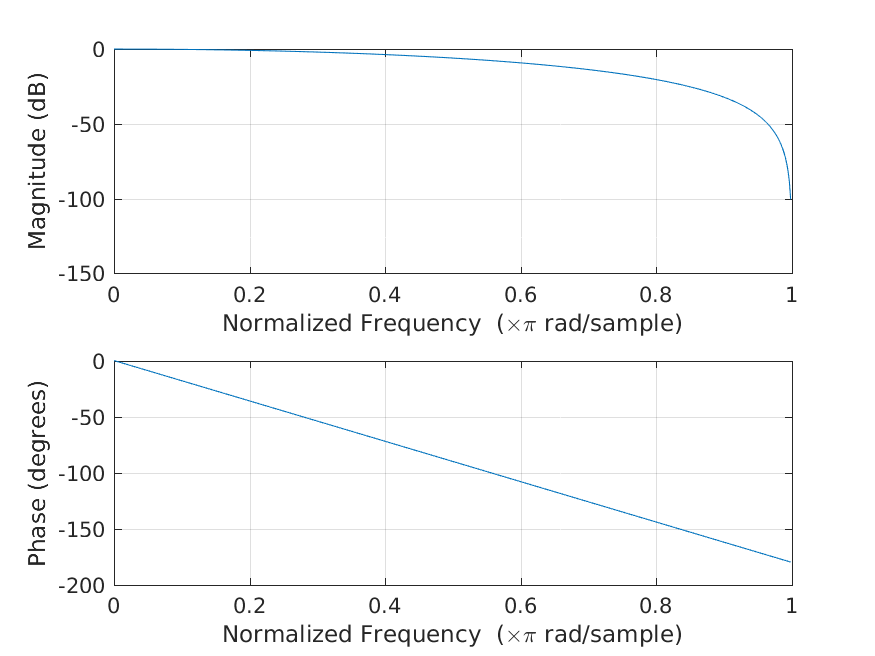
\includegraphics[width=0.45\linewidth]{figs/filter-response-hanningFilter.png} &
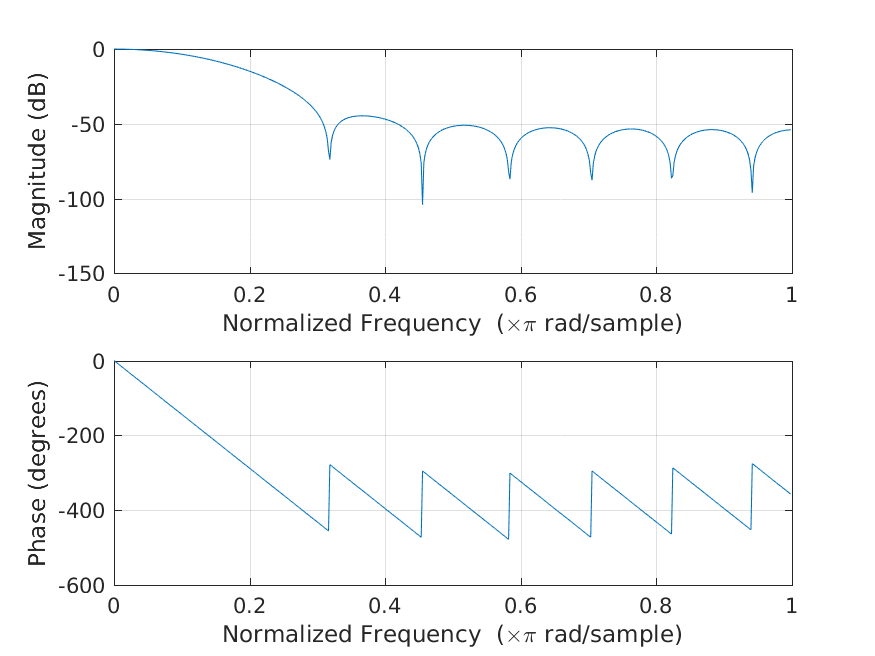
\includegraphics[width=0.45\linewidth]{figs/filter-response-wc_0_1pi.png}\\
(a) Filtro de Média móvel de Hamming & (b) Projeto com janela de Hanning $w_c=\frac{\pi}{10}$ \\
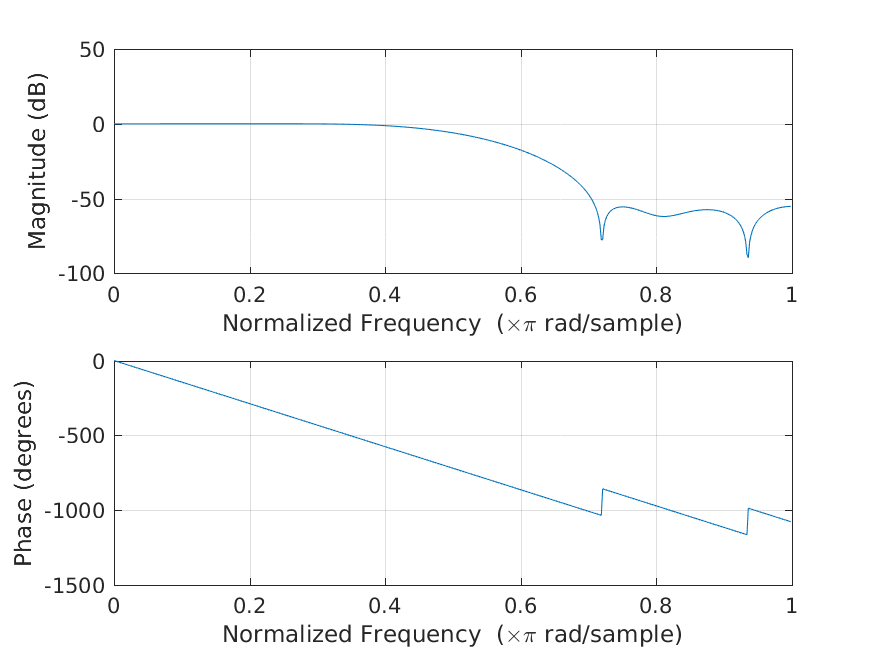
\includegraphics[width=0.45\linewidth]{figs/filter-response-wc_0_5pi.png} &
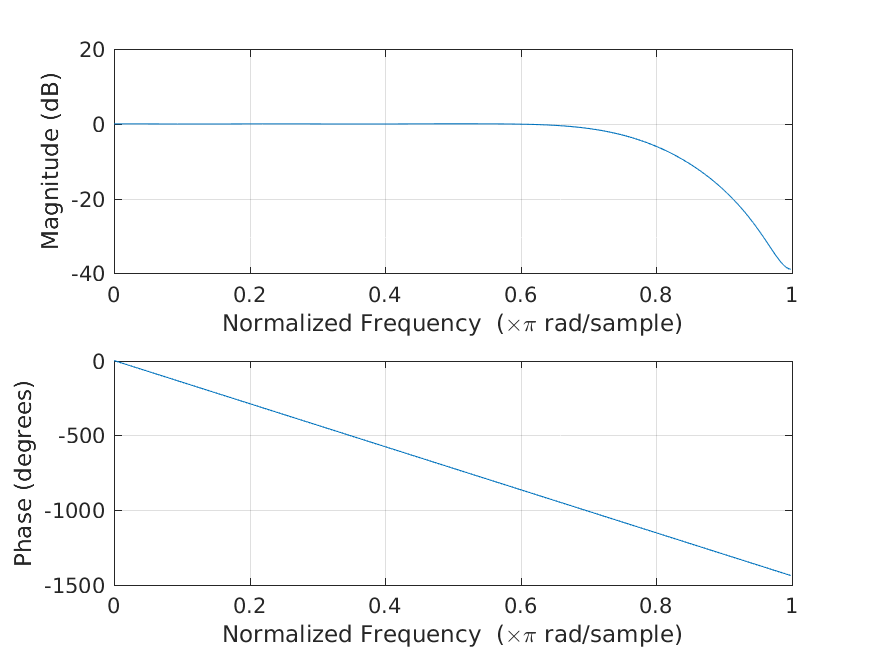
\includegraphics[width=0.45\linewidth]{figs/filter-response-wc_0_8pi.png} \\
(c) Projeto com janela de Hanning $w_c=\frac{\pi}{2}$ & (d) Projeto com janela de Hanning $w_c=\frac{4\pi}{5}$ \\
\end{tabular}

\caption{Magnitude e fase da resposta em frequência para alguns dos filtros
utilizados na aplicação.}

\label{fig:filter-design-frequency-response}
\end{figure}

\subsection{Mistura de Poses}

O conceito básico por trás da Mistura de Poses está em criar poses
intermediárias a partir da interpolação linear de poses pré-definidas.

A pose base utilizada para a mistura de poses deve ser uma onde todas as razões
de distância estão no mínimo, ou seja, deve ser uma pose onde a face esteja em
repouso. O modelo utilizado para a pose neutra é mostrada na Figura
\ref{fig:blend-shapes-base-model}.

\begin{figure*}[!htb]
   \centering
  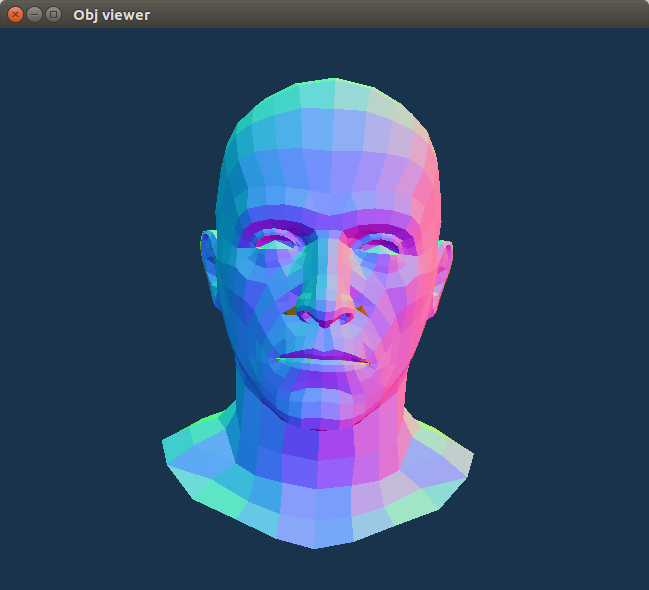
\includegraphics[width=0.8\linewidth]{./figs/rosto-neutro.png}
\caption{Pose base (neutra).}
\label{fig:blend-shapes-base-model}
\end{figure*}

Aos demais modelos renderizados é atribuído um peso de mistura definido como a
saída de um filtro que recebe como entrada uma sequência de valores de uma razão
de distância.

Alguns detalhes são necessários para que a mistura de poses ocorra com sucesso.
Dentre eles, é necessário que os pontos na malha do modelo apareçam enumerados
na mesma ordem em todas as poses utilizadas para a mistura. Isso pode ser
garantido requerendo-se do software que exporta os modelos para formato de
arquivo OBJ que mantenha os pontos na mesma ordem. Essa é uma opção comum nos
softwares de modelagem, mas que nem sempre é habilitada por padrão e o requisito
de manutenção da ordem dos pontos deve ser informado ao artista responsável pela
produção dos modelos para que ele configure o software adequadamente. Outro
requisito é que os modelos utilizem um mesmo sistema de coordenas e que os
triângulos da malha utilizem uma mesma indexação de VBOs. O primeiro requisito
não apresentou problemas na realização deste trabalho, sendo suficiente centrar
o objeto em (0,0,0), porém o segundo requisito apresentou problemas. Enquanto o
número e a ordem na listagem de triângulos se mantém o mesmo, verificou-se que
os softwares de modelagem nem sempre mantêm a mesma ordem da listagem dos pontos
de um dado triângulo. Ou seja, os pontos de um triângulo são sempre os mesmos em
dois arquivos OBJ, mas não necessariamente aparecem listados na mesma ordem, o
que causa problemas durante o processo de mistura. Para resolver este problema,
a construção da malha por meio de triângulos para todos os modelos utilizados é
feita com a listagem de triângulos da malha da pose neutra. Ou seja, os
triângulos são definidos pela pose neutra e carrega-se dos OBJ de cada uma das
outras poses apenas o posicionamento dos pontos da malha.

Caso os arquivos sejam carregados adequadamente e a mistura de poses seja
realizada com sucesso é possível verificar uma transição natural entre o modelo
da Pose Neutra para qualquer outro modelo pré-definido ao fazer a mistura de
poses utilizando-se somente a pose neutra e uma das outras poses.

Como o modelo final renderizado é uma interpolação dos pontos de todos os
modelos após a aplicação dos pesos calculados, esse modelo será igual a uma pose
pré-definida apenas se a razão de distância referente a ela for máxima, enquanto
todas as outras forem mínimas. Caso contrário, se o rosto não está em repouso, o
modelo final sempre será igual a uma pose intermediária. As poses pré-definidas
utilizadas neste trabalho são mostradas na Figura
\ref{fig:blend-shapes-base-simple-shapes1} e na Figura
\ref{fig:blend-shapes-base-simple-shapes2}.



\begin{figure}[!htpb]
  \centering
  \begin{subfigure}[Pose Olho Esquerdo]{\label{fig:pose_l_eye}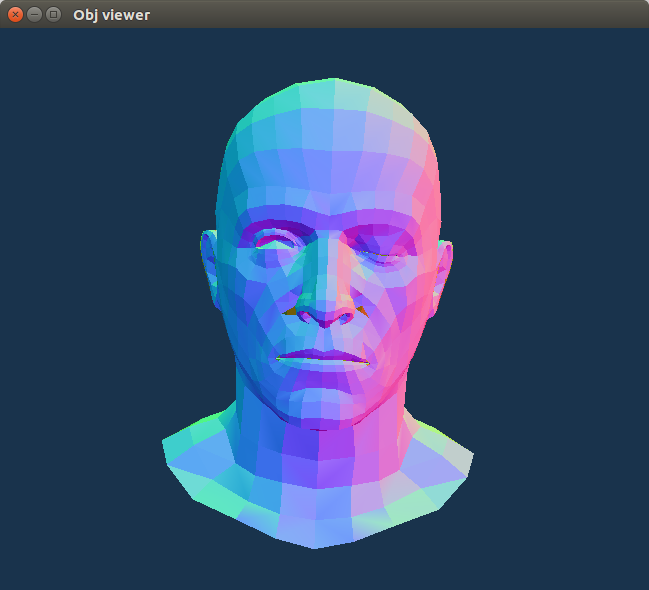
\includegraphics[width=0.4\textwidth]{./figs/left-closed-eye.png}}
  \end{subfigure}   
  \begin{subfigure}[Pose Olho Direito]{\label{fig:pose_r_eye}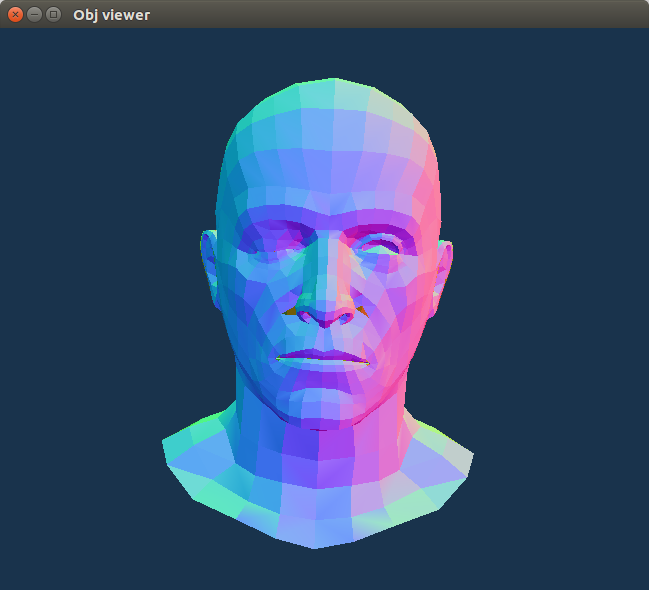
\includegraphics[width=0.4\textwidth]{./figs/right-closed-eye.png}}
  \end{subfigure}
  
  \begin{subfigure}[Pose Sobrancelha Esquerda]{  \label{fig:pose_l_eyebrow}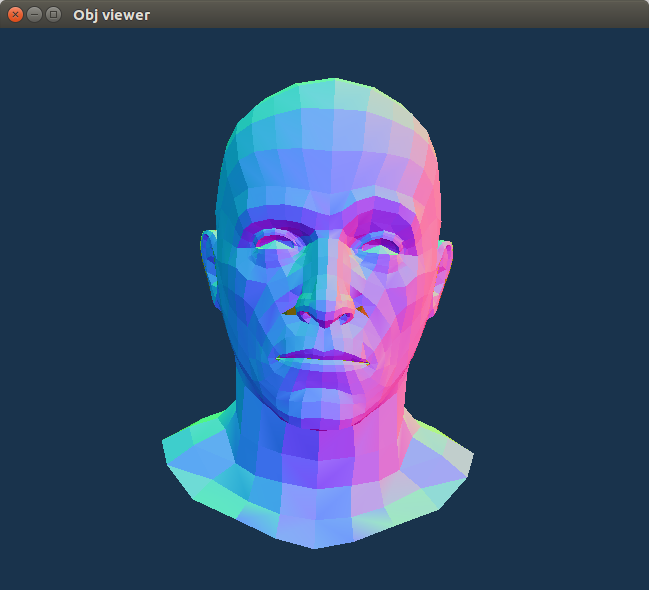
\includegraphics[width=0.4\textwidth]{./figs/left-eyebrow.png}}
  \end{subfigure} 
  \begin{subfigure}[Pose Sobrancelha Direita]{  \label{fig:pose_r_eyebrow}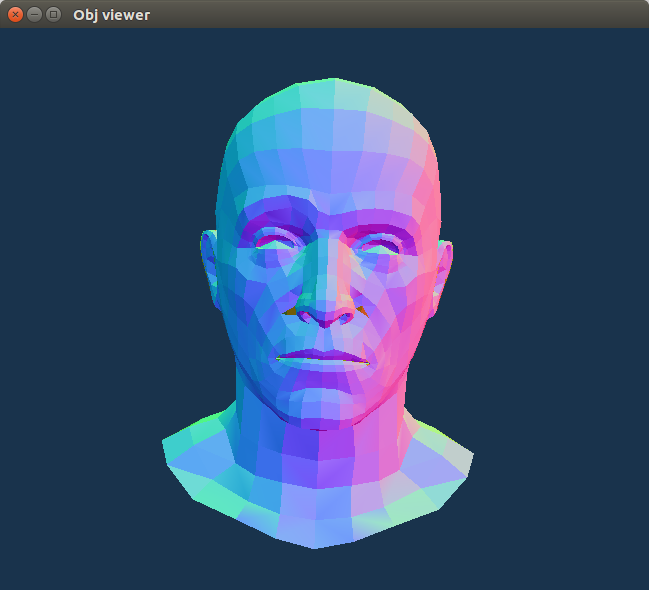
\includegraphics[width=0.4\textwidth]{./figs/right-eyebrow.png}}
  \end{subfigure}
  
  \begin{subfigure}[Pose Boca Fechada]{\label{fig:pose_c_mouth}\includegraphics[width=0.4\textwidth]{./figs/mouth-closed.png}}
  \end{subfigure}
  \begin{subfigure}[Pose Boca Aberta]{\label{fig:pose_o_mouth}\includegraphics[width=0.4\textwidth]{./figs/open-mouth.png}}
  \end{subfigure}

  \caption{Exemplos de modelos usados como poses pré definidas.}

  \label{fig:blend-shapes-base-simple-shapes1}
\end{figure}



\begin{figure}[!htpb]
  \centering
  \begin{subfigure}[Pose Bochecha Esquerda]{\label{fig:pose_l_cheek}\includegraphics[width=0.4\textwidth]{./figs/bochecha-esquerda.png}}
  \end{subfigure}   
  \begin{subfigure}[Pose Bochecha Direita]{\label{fig:pose_r_cheek}\includegraphics[width=0.4\textwidth]{./figs/bochecha-direita.png}}
  \end{subfigure}
  
  \begin{subfigure}[Pose Sorrindo]{  \label{fig:pose_happy}\includegraphics[width=0.4\textwidth]{./figs/rosto-feliz.png}}
  \end{subfigure} 
  \begin{subfigure}[Pose Bravo]{  \label{fig:pose_angry}\includegraphics[width=0.4\textwidth]{./figs/rosto-bravo.png}}
  \end{subfigure}
  
  \begin{subfigure}[Pose Nariz Aberto]{\label{fig:pose_nose}\includegraphics[width=0.4\textwidth]{./figs/nose.png}}
  \end{subfigure}

  \caption{Exemplos de modelos usados como poses pré definidas.}

  \label{fig:blend-shapes-base-simple-shapes2}
\end{figure}

A Equação \ref{eq:blendshapes} descreve como as poses pré-definidas podem ser
combinadas com a pose neutra de forma a obter  uma quantidade imensa de poses
intermediárias. 

Conectando as etapas apresentas até agora dentro de um laço de execução, os
pesos de mistura são atualizados iterativamente de acordo com o movimento dos
pontos rastreados, produzindo mudanças suaves na forma do modelo resultante
renderizado. A sequência de configurações pelas quais passa o modelo renderizado
a medida que as imagens são capturadas e processadas resultam na animação
computacional que é o objetivo da aplicação.


% O resultado dessa animação pode ser observado na Figura \ref{fig:final_model1}, onde o modelo final é uma pose intermediária entre, essencialmente, o modelo de sorriso e o modelo de boca aberta.

% \begin{figure*}[!htb]
%    \centering
% \begin{tabular}{cc}
%   \includegraphics[width=0.4\linewidth]{./figs/mouth-closed.png}
%   \includegraphics[width=0.4\linewidth]{./figs/rosto-bravo.png}
% \end{tabular}

% \caption{legenda}

% \label{fig:blend-shapes-base-complex-shapes}
% \end{figure*}

% \begin{figure*}[!htb]
%    \centering
% \begin{tabular}{cc}
%   \includegraphics[width=0.4\linewidth]{./figs/TG_pose_inter_input1.png}
%   \includegraphics[width=0.4\linewidth]{./figs/TG_pose_inter_model1.png}
% \end{tabular}

% \caption{legenda}

% \label{fig:final_model1}
% \end{figure*}

\section{Experimentos de Validação dos Métodos Utilizados}

Como não se dispõe de um método para medir a qualidade final dos resultados de
modo quantitativo, propõem-se alguns experimentos com o objetivo de validar as
etapas do processo. Os experimentos visam revelar as limitações atuais da
técnica ao medir a precisão de cada etapa.

Uma das dificuldades enfrentadas no experimento é que a aplicação envolve o
rastreamento de um rosto humano e não é encontrada uma boa maneira de substituir
o alvo humano por um objeto que possa ser facilmente fixado e ter a posição
controlada. Com isso, pessoas são utilizadas como parte do experimento e
certamente há erros introduzidos nas medidas. Para exemplificar, em um dos
experimentos propostos o objetivo é tirar várias fotos do usuário há uma
distância fixa, no entanto, é difícil garantir que o alvo não tenha se movido
entre uma foto e outra. Há ainda o problema da iluminação que pode variar
ligeiramente a medida que as horas de experimentos passam. Tendo isso em mente,
o objetivo dos experimentos é que eles forneçam uma ideia das limitações da
técnica e não que sejam uma metodologia precisa de estimação dos erros
envolvidos.

A Figura \ref{fig:exp-montagem} mostra a montagem utilizada nos experimentos que
se seguem. Antes de cada medida, os passos a seguir são tomados como uma
configuração inicial:

\begin{enumerate}

\item O par de câmeras é posicionado na altura do rosto alvo. Seja a direção da
  linha ligando as câmeras chamada de $\vec{A}$.

\item A ponta da trena horizontal é posta no ponto médio entre as câmeras e é
  puxada em direção $\vec{B}$ perpendicular a $\vec{A}$ e no sentido apontando
  para o usuário.

\item O usuário segura a trena e se afasta do par de câmeras se movendo na
  direção $\vec{B}$ até atingir a distância desejada.

\item Nesse ponto uma segunda régua (segmento vermelho na Figura
  \ref{fig:exp-montagem}) é posta verticalmente e ortogonalmente sobre a trena e
  o usuário encosta o nariz na ponta da régua vertical. 

\item Esta é a posição que o ator deve manter durante o resto do experimento o
  mais fielmente possível.

\end{enumerate}

\begin{figure}[!htp]
\centering
\includegraphics[width=0.8\linewidth]{figs/setupExperimento-comentado.png}
\caption{\textit{Setup} experimental utilizado para captura repetitiva de fotos do mesmo alvo em várias posições controladas.}
\label{fig:exp-montagem}
\end{figure}

\subsection{Rastreamento de Pontos da Face e Estimação do Tridimensional}

O Rastreamento de Pontos da Face retorna o valor das coordenadas dos pontos em
pixeis, fazendo com que as distâncias entre pares de pontos associados a uma
pose, quando avaliadas diretamente na imagem, mudem à medida que o usuário se
afasta ou se aproxima do sistema de captura. Por outro lado, a técnica de
estimação de profundidade almeja garantir que essas distâncias, agora medidas em
centímetros, se mantenham as mesmas se as distâncias assim se mantiverem no
objeto real. Para mostrar que a recuperação da profundidade está sendo feita de
forma adequada, propõe-se um experimento que irá medir a distância em
centímetros de um par de pontos do rosto, à medida que o usuário se afasta do
par de câmeras. Se o processo for feito como esperado, a distância entre os
pontos do rosto será sempre a mesma, independentemente das distância do alvo às
câmeras.  Outro ponto a ser notado é que para o rastreamento ser considerado
preciso, as distâncias medidas não podem variar no caso de o face alvo estar
imóvel. Para verificar isso, propõe-se também medir o desvio padrão na sequência
de medidas de distância entre dois pontos de uma face imóvel em uma série de
capturas.


Para ambos os experimentos o par de pontos escolhidos para se medir em cada
quadro é composto pelos pontos laterais extremos dos lábios (pontos 48 e 54 na
Figura \ref{fig:tracked-facial-points}). As mesmas imagens capturadas foram
utilizadas em ambos os experimentos.

Para a realização dos experimentos, os seguintes passos foram tomados:

\begin{enumerate}
      
\item A montagem inicial é executada posicionando o nariz do alvo a 40
  centímetros de distância.

\item Capturam-se 30 quadros de cada câmera enquanto o alvo se mantém o mais
  estático possível.

\item Repete-se o processo afastando-se o alvo do par de câmeras 5 centímetros
  em cada etapa, até que se atinja a distância de 80 cm do par de câmeras.

\end{enumerate}

Após a captura, as imagens são entradas aos pares em um programa que:

\begin{enumerate}

\item Aplica o algoritmo de rastreamento dos 66 pontos do rosto no par de
  imagens.

\item Mede a distância entre os pontos 48 e 54 em pixeis para cada câmera.

\item Aplica a técnica de estimação de profundidade para corrigir as coordenadas
  (x,y) de cada ponto detectado

\item Mede a distância entre os pontos 48 e 54 em centímetros.

\end{enumerate}

Para cada par de quadros, os seguintes valores são salvos em arquivo: a
distância entre os pontos 48 e 54 em pixeis da imagem capturada com a câmera 1,
a distância entre os pontos 48 e 54 em pixeis da imagem capturada com a câmera 2
e a distância entre os pontos 48 e 54 estimada em centímetros. 


\subsection{Filtragem Digital}

Neste experimento o objetivo é comparar a sequência de coeficientes de mistura
filtrada e não-filtrada.  Para cada um dos pesos de mistura grava-se um par de
vídeos, um para cada câmera, onde o ator centrado na tela movimenta
intencionalmente os músculos do rosto associados com o peso de mistura que se
quer examinar. 

Apenas um vídeo é gravado para cada pose examinada. Todos os vídeos são gravados
a uma mesma distância da câmera e sobre condição de iluminação semelhante. No
caso de poses simétricas, como o fechar do olho esquerdo e do direito, apenas o
movimento do lado esquerdo do rosto é examinado. Para cada movimento avaliado,
os vídeos gravados são colocados em um programa que aplica o rastreamento visual
dos pontos do rosto e mede apenas a razão de distância considerada (por exemplo,
no vídeo que examina o olho, mede-se somente a abertura dos olhos e no vídeo que
examina o sorrir, apenas o comprimento horizontal dos lábios é medido). 

A razão obtida é entrada independentemente em cada um dos filtros projetados. A
razão medida e a saída de cada um dos filtros é guardada em arquivo para análise
posterior.

O próximo capítulo apresenta os resultados obtidos neste trabalho, para cada etapa 
intermediária e para o sistema de animação completo em funcionamento.




\chapter{Resultados}

Este capítulo apresenta os resultados obtidos nos experimentos feitos para validação das técnicas utilizadas neste trabalho, bem como o resultado final da aplicação.

É importante notar que apesar da limitação dos experimentos feitos para o rastreamento de pontos do rosto e para a estimação tridimensional foi possível obter dados suficientes para uma análise de precisão das técnicas.

\section{Calibração das Câmeras}

A Tabela \ref{tab:params_intrisecos} mostra os parâmetros intrínsecos das câmeras utilizadas obtidos utilizando a ferramenta \textit{Camera Calibration Toolbox for Matlab}.

\begin{table}[!htb]
\centering
\begin{tabular}{|c|c|c|}
\hline
Parâmetros intrínsecos & Câmera 1 (pixel) & Câmera 2 (pixel)\\ \hline
$f_c(1)$ & $854 \pm 4$ &  $834 \pm 6$ \\ \hline
$f_c(2)$ & $858 \pm 4$ & $836 \pm 6$ \\ \hline
$cc(1)$ & $298 \pm 6$ & $300 \pm 7$ \\ \hline
$cc(2)$ & $232 \pm 6$ & $217 \pm 7$ \\ \hline
$alpha_c$ & 0 & 0 \\ \hline
\end{tabular}

\caption{Parâmetros intrínsecos da câmera medidos em pixeis.}
\label{tab:params_intrisecos}
\end{table}

Como pode ser observado os valores de $f_c(1)$ e $f_c(2)$, referentes a distância focal medida em pixeis horizontais e verticais, são bem próximos para ambas as câmeras. Com isso pode-se assumir que a câmera possui um pixel quadrado e assim tem uma distância focal $f = (f_c(1) + f_c(2))/2$, sendo $f$ o valor em pixeis.

As câmeras utilizadas neste trabalho são do mesmo modelo e seu foco é ajustável. O foco das câmeras foi ajustado para ficar parecido, a partir de uma avaliação visual apenas. Todos estes fatores explicam os resultado similares obtidos para as duas câmeras.

A partir destes dados é possível estimar a profundidade de um ponto alvo utilizando a Equação \ref{eq:3d_Zequation} e assim estimar o valor de $X$ em centímetros, pelas Equações \ref{eq:3d_realX1} e \ref{eq:3d_realX1}, assim como estimar o valor de $Y$ em centímetros, pelas Equações \ref{eq:3d_realY1} e \ref{eq:3d_realY2}.

\section{Rastreamento de Pontos da Face}

Os experimentos realizados nesta seção foram feitos com o objetivo de avaliar a precisão da detecção de pontos da face utilizando a SDK \textit{CSIRO Face Analysis}, bem como justificar o uso de técnicas de estimação tridimensional e filtragem digital.

Duas poses foram avaliadas, a Pose Neutra e a Pose Sorrindo, com isso a razão de distância avaliada foi a do \textbf{comprimento dos lábios}, já que é essa razão que varia entre as poses e que consequentemente, após a filtragem, se torna um dos pesos aplicados ao modelo final.

Para ambas câmeras 1 e 2 foi obtida a média e o desvio padrão para essa razão de distância, em pixeis, a partir de vários valores de profundidade. A média e o desvio padrão foram calculados a partir do valores medidos em trinta imagens de uma face imóvel capturadas sucessivamente com intervalos de tempo menores que um segundo.

A Tabela \ref{tab:exp-px-variando-dist-cam1} exibe os valores obtidos através da câmera 1. Enquanto a Figura \ref{fig:graf-cam1-dsv-dist} mostra um gráfico da variação do desvio padrão do comprimento dos lábios, para a Pose Neutra e a para Sorrindo, em relação a distância entre a câmera 1 e o alvo.


\begin{table}[!htb]
\centering
\begin{tabular}{|*{6}{>{\centering\arraybackslash}p{.16\linewidth}|}}
\cline{2-5}
	\multicolumn{1}{c|}{} & \multicolumn{2}{c|}{Câmera 1 - Pose Neutra (pixel)} & \multicolumn{2}{c|}{Câmera 1 - Pose Sorrindo (pixel)} \\ \hline
    \begin{tabular}{@{}c@{}}Distância da \\ câmera (cm)\end{tabular} & Média &  Desvio padrão & Média &  Desvio padrão \\ \hline
40 & 93.4096 & 0.5575 & 92.1488 & 1.3473 \\ \hline
45 & 83.7242 & 0.6406 & 84.694  & 0.8848 \\ \hline
50 & 75.6548 & 0.7163 & 78.1044 & 1.0881 \\ \hline
55 & 67.9294 & 0.6772 & 69.1071 & 0.9671 \\ \hline
60 & 65.1105 & 0.3884 & 65.8582 & 0.8114 \\ \hline
65 & 58.8054 & 0.3392 & 59.7229 & 0.5219 \\ \hline
70 & 54.7137 & 0.5925 & 55.7597 & 0.6367 \\ \hline
75 & 53.4555 & 0.4781 & 53.7684 & 0.6277 \\ \hline
80 & 49.1185 & 0.3156 & 49.7219 & 0.2373 \\ \hline
\end{tabular}
\caption{Comprimento horizontal dos lábios medido em pixeis a partir de imagens capturadas do rosto alvo pela câmera 1 em distâncias variáveis.}
\label{tab:exp-px-variando-dist-cam1}
\end{table}

\begin{figure}[!htb]
\centering
\includegraphics[width=0.8\textwidth]{figs/thumbnail_cameraEsquerda.jpg} 
\caption{Gráfico da variação do desvio padrão, em pixeis, em relação a distância, em centímetros, de pontos rastreados nas imagens capturadas pela câmera 1.}
\label{fig:graf-cam1-dsv-dist}
\end{figure}

A Tabela \ref{tab:exp-px-variando-dist-cam2} exibe os valores obtidos através da câmera 2. Enquanto a Figura \ref{fig:graf-cam2-dsv-dist} mostra um gráfico da variação do desvio padrão do comprimento dos lábios, para a Pose Neutra e a para Sorrindo, em relação a distância entre a câmera 2 e o alvo.

\begin{table}[!htb]
\centering
\begin{tabular}{|*{6}{>{\centering\arraybackslash}p{.16\linewidth}|}}
\cline{2-5}
	\multicolumn{1}{c|}{} & \multicolumn{2}{c|}{Câmera 2 - Pose Neutra (pixel)} & \multicolumn{2}{c|}{Câmera 2 - Pose Sorrindo (pixel)} \\ \hline
    \begin{tabular}{@{}c@{}}Distância da \\ câmera (cm)\end{tabular} & Média &  Desvio padrão & Média &  Desvio padrão \\ \hline
40 & 92.1488 & 1.3473 & 119.6076 & 2.2723 \\ \hline
45 & 84.694  & 0.8848 & 106.7452 & 2.23   \\ \hline
50 & 78.1044 & 1.0881 & 108.4763 & 1.2881 \\ \hline
55 & 69.1071 & 0.9671 & 94.7001  & 1.2003 \\ \hline
60 & 65.8582 & 0.8114 & 87.5216  & 0.5491 \\ \hline
65 & 59.7229 & 0.5219 & 82.719   & 0.9558 \\ \hline
70 & 55.7597 & 0.6367 & 75.3994  & 0.4099 \\ \hline
75 & 53.7684 & 0.6277 & 67.9172  & 1.0836 \\ \hline
80 & 49.7219 & 0.2373 & 68.2629  & 1.0946 \\ \hline
\end{tabular}
\caption{Comprimento horizontal dos lábios medido em pixeis a partir de imagens capturadas do rosto alvo pela câmera 2 em distâncias variáveis.}
\label{tab:exp-px-variando-dist-cam2}
\end{table}

\begin{figure}[!htb]
\centering
\includegraphics[width=0.8\textwidth]{figs/thumbnail_cameraDireita.jpg} 
\caption{Gráfico da variação do desvio padrão, em pixeis, em relação a distância, em centímetros, de pontos rastreados nas imagens capturadas pela câmera 2.}
\label{fig:graf-cam2-dsv-dist}
\end{figure}

Os gráficos exibidos na Figura \ref{fig:graf-cam1-dsv-dist} e na Figura \ref{fig:graf-cam2-dsv-dist} mostram que existe uma instabilidade no rastreamento de pontos da face, que apesar de pequena pode afetar o modelo final. Essa variação dos pontos acontecem em altas frequências, visto que as imagens foram capturadas sucessivamente em pequenos intervalos de tempo, assim essa instabilidade pode ser tratada com a utilização de filtragem digital. 

Outro comportamento exibido pelos gráficos é o de que o desvio padrão é quase sempre maior quando a razão de distância é medida na Pose Sorrindo do que quando ela é medida na Pose Neutra, ou seja, o rastreamento geralmente é mais estável quando feito em uma face sem expressões.

Como observado o desvio padrão em geral diminui com o aumento da distância, porém esse acontecimento pode ser atribuído ao fato de que, como a razão de distância esta avaliada em pixeis, quanto maior a distância menor o valor da razão de distância.

Observando as tabelas é possível reparar na diminuição drástica da média a medida que o valor de profundidade aumenta, de forma que o valor obtido do comprimento dos lábios a uma distância de 80cm é quase a metade do valor a 40cm. 

Essa mudança brusca impossibilita uma boa calibração para as razões de distância, visto que a razão de distância, e consequentemente o modelo final, pode mudar com uma variação de profundidade, mesmo se o alvo estiver na mesma pose. Para isso é usada a estimação tridimensional, com ela é possível manter uma mesma razão de distância, caso a pose seja a mesma, não importa a profundidade, não alterando assim o modelo final.

\section{Estimação do Tridimensional}

O objetivo dos experimentos nessa seção é avaliar a precisão da técnica de estimação tridimensional. Deve-se notar que uma precisão na estimação do $X$ e do $Y$ no sistema de coordenadas do mundo só é possível caso haja precisão na estimação do $Z$, como pode ser observado nas Equações \ref{eq:3d_realX1}, \ref{eq:3d_realX2}, \ref{eq:3d_realY1} e \ref{eq:3d_realY2}.

Como nos experimentos da seção anterior, em que foi avaliada a precisão do rastreamento de pontos da face, a razão de distância analisada foi a referente ao comprimento dos lábios. Foram utilizadas as mesmas imagens, porém agora essa razão de distância foi estimada em centímetros, ou seja os pontos foram estimados no sistema de coordenadas do mundo.

A Tabela \ref{tab:exp-px-variando-dist-3d} exibe os valores estimados em centímetros. Enquanto a Figura \ref{fig:graf-3d-dsv-dist} e a Figura \ref{fig:graf-3d-media-dist} mostram um gráfico da variação do desvio padrão e da média, respectivamente, do comprimento dos lábios, para a Pose Neutra e a para Sorrindo, em relação a distância entre as câmeras e o alvo.


\begin{table}[!htb]
\centering
\begin{tabular}{|*{6}{>{\centering\arraybackslash}p{.16\linewidth}|}}
\cline{2-5}
	\multicolumn{1}{c|}{} & \multicolumn{2}{c|}{Pose Neutra (cm)} & \multicolumn{2}{c|}{ Pose Sorrindo (cm)} \\ \hline
    \begin{tabular}{@{}c@{}}Distância da \\ câmera (cm)\end{tabular} & Média &  Desvio padrão & Média &  Desvio padrão \\ \hline
40 & 5.2755 & 0.1155 & 6.8652 & 0.2549 \\ \hline
45 & 5.5857 & 0.0991 & 6.8311 & 0.1564 \\ \hline
50 & 5.4356 & 0.0959 & 7.3474 & 0.116  \\ \hline
55 & 5.3663 & 0.1135 & 7.3599 & 0.1574 \\ \hline
60 & 5.5722 & 0.1144 & 7.4396 & 0.1107 \\ \hline
65 & 5.4381 & 0.0932 & 7.4996 & 0.1433 \\ \hline
70 & 5.8243 & 0.0879 & 7.7648 & 0.1024 \\ \hline
75 & 5.7759 & 0.1494 & 7.1711 & 0.2339 \\ \hline
80 & 5.5645 & 0.0716 & 7.7803 & 0.1659 \\ \hline
\end{tabular}
\caption{Comprimento horizontal dos lábios medido em centímetros a partir de imagens capturadas do rosto alvo em distâncias variáveis.}
\label{tab:exp-px-variando-dist-3d}
\end{table}

\begin{figure}[!htpb]
\centering
\includegraphics[width=0.8\textwidth]{figs/thumbnail_distanciaCorrigida.jpg} 
\caption{Gráfico da variação do desvio padrão, em centímetros, em relação a distância, em centímetros, de pontos estimados no sistema de coordenadas do mundo.}
\label{fig:graf-3d-dsv-dist}
\end{figure}

O gráfico exibido na Figura \ref{fig:graf-3d-dsv-dist} mostra o desvio padrão do valor em centímetros da razão de distância, ele pode ser diretamente relacionado com a instabilidade do rastreamento de pontos. Essa instabilidade é exibida na Figura \ref{fig:graf-cam1-dsv-dist} e na Figura \ref{fig:graf-cam2-dsv-dist}. 

\begin{figure}[!htpb]
\centering
\includegraphics[width=0.8\textwidth]{figs/media3d.png} 
\caption{Gráfico da variação média, em centímetros, em relação a distância, em centímetros, de pontos estimados no sistema de coordenadas do mundo.}
\label{fig:graf-3d-media-dist}
\end{figure}

A precisão da estimação tridimensional pode ser verificada ao se avaliar a variação da média em relação a distância. Esses dados são exibidos na Figura \ref{fig:graf-3d-media-dist}, nota-se que a média se mantém suficientemente constante, principalmente nos intervalos entre 50cm e 65cm. Com isso pode-se concluir que mesmo que aconteça uma variação da distância do alvo em relação as câmeras, a razão de distância se manterá estável, garantindo estabilidade para o modelo final.

\section{Filtros}

Neste experimentos foram gerados gráficos de sequências para os pesos de mistura de 3 das poses utilizadas. Cada gráfico mostra medidas de pesos de mistura para uma das poses, com um curva para os valor não-filtrado e curvas para alguns dos filtros projetados.  As sequências foram obtidas em um vídeo gravado com o objetivo de movimentar especificamente a pose sendo testada. Os gráficos foram gerados selecionando-se parte das sequências gravadas.

A Figuras \ref{fig:filter-left-eye}, \ref{fig:filter-open-mouth} e \ref{fig:filter-smile} demonstram a atuação dos filtros sobre a variação do peso de mistura para as poses Olho Esquerdo, Boca Aberta e Sorriso.

\begin{figure}[!htb]
\centering
\includegraphics[width=1.0\textwidth]{figs/filter-result-open-mouth.pdf} 
\caption{Peso de mistura para a Pose Olho Esquerdo}
\label{fig:filter-left-eye}
\end{figure}

\begin{figure}[!htb]
\centering
\includegraphics[width=0.8\textwidth]{figs/filter-result-left-eye.pdf} 
\caption{Peso de mistura para a Pose Boca Aberta}
\label{fig:filter-open-mouth}
\end{figure}

\begin{figure}[!htb]
\centering
\includegraphics[width=0.8\textwidth]{figs/filter-result-smile-2.pdf} 
\caption{Peso de mistura para a Pose Sorriso}
\label{fig:filter-smile}
\end{figure}

Como visto nas Figuras \ref{fig:graf-cam1-dsv-dist} e \ref{fig:graf-cam2-dsv-dist} o rastreamento em si não é totalmente preciso nem quando o rosto está imóvel, logo em um vídeo longo onde ocorre movimentação e variação de luminosidade é esperado que o sinal sem filtragem seja mais ruidoso, como é mostrados no gráficos. 

A filtragem suaviza o sinal e consequentemente melhora a animação final. Vários tipos de filtro foram analisados e seus desempenhos foram variados.

Como pode ser observado os filtros projetados pela técnica de janela acabam atrasando atrasando o sinal e, apesar de eles serem eficientes em filtrar altas frequências, esses tipos de filtro acabam prejudicando a performance da animação em tempo real.

Por outro lado o filtro de hanning conseguiu seguir o sinal original e manter uma boa filtragem das altas frequências, isso acontece pois este tipo de filtro possui muito menos parâmetros que os outros projetados. Para este trabalho, onde um dos objetivos é a animação em tempo real, esse tipo filtro apresentou o melhor resultado.

\section{Mistura de Poses}

Neste experimento foi avaliada somente a técnica de mistura de poses, ou seja, foi renderizado um modelo final sem a influência do rastreamento de pontos da face. Para isso foram atribuídos manualmente os valores de peso.

Alguns exemplos de modelos finais de poses intermediárias renderizados com sucesso podem ser vistos na Figura \ref{fig:blend-shapes-inter-simple-shapes}.

\begin{figure}[!htb]
  \centering
  \begin{subfigure}[]{\label{fig:inter1}\includegraphics[width=0.4\textwidth]{./figs/TG_angry60_leftcheek75_lefteye55_closemouth35.png}}
  \end{subfigure}   
  \begin{subfigure}[]{\label{fig:inter2}\includegraphics[width=0.4\textwidth]{./figs/TG_happy40_righteyebrow95_openmouth60.png}}
  \end{subfigure}
  
  \begin{subfigure}[]
  {\label{fig:inter3}\includegraphics[width=0.4\textwidth]{./figs/TG_lefteye100_rigtheye100_openmouth60.png}}
  \end{subfigure} 
  \begin{subfigure}[]
  {\label{fig:inter4}\includegraphics[width=0.4\textwidth]{./figs/TG_happy70_angry90.png}}
  \end{subfigure}
  
  \begin{subfigure}[]{\label{fig:inter5}\includegraphics[width=0.4\textwidth]{./figs/TG_angry100_openmouth90.png}}
  \end{subfigure}
  \begin{subfigure}[]{\label{fig:inter6}\includegraphics[width=0.4\textwidth]{./figs/TG_angry100_leftcheek100_rightcheek65_closemouth100.png}}
  \end{subfigure}

  \caption{Exemplo de misturas geradas configurando os parâmetros de mistura manualmente. Pesos da Figura \ref{fig:inter1}: Olho Esquerdo - 0.55, Boca Fechada - 0.35, Bochecha Esquerda - 0.75 e Bravo - 0.6. Pesos da Figura \ref{fig:inter2}: Sobrancelha Direita - 0.95, Boca Aberta - 0.6 e Sorrindo - 0.4. Pesos da Figura \ref{fig:inter3}: Olho Esquerdo - 1.0, Olho Direito - 1.0 e Boca Aberta - 0.6. Pesos da Figura \ref{fig:inter4}: Sorrindo - 0.7 e Bravo - 0.6. Pesos da Figura \ref{fig:inter5}: Boca Aberta - 1.0 e Bravo - 0.9. Pesos da Figura \ref{fig:inter6}: Boca Fechada - 1.0, Bochecha Esquerda - 1.0, Bochecha Direita - 0.65, e Bravo - 1.0.}

  \label{fig:blend-shapes-inter-simple-shapes}
\end{figure}

Como pode ser observado nos modelos finais exibidos a técnica de mistura de poses teve ótimos resultados. 

A indexação dos VBOs e a ordenação dos vetores foi constante, pois se não sendo este o caso seria possível observar algumas falhas óbvias no modelo, como alguns buracos aparecendo ou deformações irregulares se formando.

As significância de cada pose pré-definida no modelo final está bem relacionada com os pesos aplicados e essa relação pode ser claramente visualizada nas figuras, ou seja, ao aplicar a Equação \ref{eq:blendshapes} é possível criar, a partir de poucas poses pré-definidas, uma quantidade enorme de poses intermediárias significativamente diferentes.

Com esses resultados pode se concluir que caso ocorra uma boa estimação das razões de distância, a partir de um rastreamento de pontos, estimação tridimensional e filtragem, o modelo final correto será renderizado com sucesso.

\section{Sistema em Funcionamento}

A avaliação do sistema em funcionamento, similarmente ao que foi feito para a mistura de poses, é qualitativa. Quadros comparativos entre a imagem de entrada e o modelo final foram exibidos na \ref{fig:sist-func}, de forma a observar a qualidade da animação, avaliando o impacto do movimento dos pontos utilizados como referências para as razões de distância no modelo final. Para isso é necessária uma boa calibração dos valores de distância mínima e máxima para cada razão de distância. Esta avaliação é porém embasada nos resultados dos experimento obtidos para cada etapa.

O sistema em funcionamento pode ser observado na Figura \ref{fig:sist-func} em que o modelo final segue os movimentos do rosto alvo a partir das razões de distância consideradas.

\begin{figure}[!htb]
  \centering
  \begin{subfigure}[]{\label{fig:inter1}\includegraphics[width=0.35\textwidth]{./figs/TG-resultado-par-4-img-1.png}}
  \end{subfigure}   
  \begin{subfigure}[]{\label{fig:inter2}\includegraphics[width=0.35\textwidth]{./figs/TG-resultado-par-4-img-2.png}}
  \end{subfigure}
  
  \begin{subfigure}[]
  {\label{fig:inter3}\includegraphics[width=0.35\textwidth]{./figs/TG-resultado-par-5-img-1.png}}
  \end{subfigure} 
  \begin{subfigure}[]
  {\label{fig:inter4}\includegraphics[width=0.35\textwidth]{./figs/TG-resultado-par-5-img-2.png}}
  \end{subfigure}

  \caption{Imagens que demonstram o sistema em funcionamento.}

  \label{fig:sist-func}
\end{figure}




\chapter{Conclusões}

\label{CapConclusoes}

Desenvolveu-se um sistema que permite transferir um conjunto de movimentos
faciais para um avatar computacional a partir de uma sequência de imagens
capturadas por um par de câmeras. O sistema realiza a tarefa utilizando
\textit{webcams} simples e não exige um ambiente controlado, marcadores no
usuário ou mesmo uso de iluminação especial. Para se ter uma ideia da robustez
dos resultados, o sistema foi testado com sucesso em ambientes como uma sala de
escritório e até mesmo a sala de estar de um dos autores.

Os movimentos independentemente transferidos incluem: sorrir, abrir a boca,
fechar os olhos e levantar as sobrancelhas. A técnica chave utilizada foi
conectar características de um conjunto de pontos obtidos de um processo de
rastreamento visual com os pesos de mistura da técnica de Mistura de Poses,
permitindo gerar expressões variadas para o avatar a partir da combinação de um
conjunto reduzido de expressões chave. 

Para o rastreamento visual, utilizou-se a biblioteca FaceAnalysis SDK para
capturar 66 pontos chaves do rosto humano em uma sequência de imagens. Já para
gerar os pesos de mistura, foi utilizada uma regra simples baseada na razão
entre distâncias de pontos nomeados. Com o objetivo de tornar o processo robusto
à distância do usuário ao par de câmeras, se utilizou estimação de
tridimensionalidade para tornar os pesos de mistura uma função das distâncias
reais entre os pontos e não das distâncias em pixeis das câmeras. Para isso, foi
preciso uma etapa prévia de calibração das câmeras utilizadas.

Além disso, com o intuito de suavizar os resultados ao eliminar ruídos, os pesos
de mistura passam por um filtro digital. Dois tipos de filtros foram utilizados:
um filtro de de média móvel de Hanning de comprimento três e um conjunto de
filtros projetados pela técnica de corte de janela.  Apesar de muito menos
elaborado, o primeiro filtro apresentou melhores resultados que os últimos.
Entende-se que o ruído presente no sinal não possui comportamento espectral que
justifique um projeto cuidadoso de um filtro passa-baixas. Um filtro curto, que
ainda assim atenue frequências altas, performa melhor por impor um atraso menor
no sinal de saída.

Uma série de experimentos foi realizada com o objetivo de medir a confiança
em cada etapa do processo. A partir desses experimentos pôde-se inferir a
distância que o usuário deve se posicionar do par de câmeras para que a técnica
transfira os movimentos para o avatar de forma mais efetiva. Outro resultado foi
que apesar de adequada para capturar o movimento da boca e das sobrancelhas, a
regra associativa entre pontos e pesos de mistura não foi capaz de capturar
outros movimentos faciais, como o movimento de bochechas e o piscar dos olhos.
Isso se deve, em parte, à certa rigidez do algoritmo de rastreamento utilizado
quanto ao formato do rosto, o que impede que este seja aplicado, pelo menos
diretamente, para capturar nuâncias de certas expressões. Com isso, algumas das
poses chave disponíveis não foram utilizadas na aplicação final.

Os resultados obtidos mostram a validade da técnica. Por exemplo, o programa
desenvolvido foi capaz de sincronizar a abertura e o fechamento da boca do
avatar enquanto o usuário conversava com a câmera em um dos vídeos de teste.
Além disso, quando executando em máquinas comuns e ligado diretamente nas
câmeras, o programa mostra os resultados em tempo de execução sem atraso
perceptível entre entrada e saída. Por rodar em máquinas ordinárias, não exigir
longas horas de processamento e não exigir controle especial do ambiente de
filmagem a metodologia proposta se confirma como uma de baixo custo.



\section{Trabalhos Futuros}

A técnica de mistura de poses chaves se mostrou uma maneira simples de gerar
expressões complexas a partir de medidas simples obtidas em uma imagem. No
entanto, na implementação atual os pontos na malha das poses chaves estão
limitados a serem os mesmos dos pontos da pose base a menos de uma translação.
Com isso não pode-se animar uma pose chave onde, por exemplo, o avatar vira o
pescoço. A geometria vetorial na mistura de poses não funcionaria adequadamente.
É possível aplicar a técnica de mistura de poses com rotação dos pontos do
modelo, desde que se conheça a transformação completa que deve ocorrer em cada
ponto, não apenas sua translação. Uma possível direção para o trabalho seria
implementar estas transformações e as misturas delas. Nota-se que isso
implicaria, possivelmente, em mudar a representação dos modelos e acarretaria
maior custo na renderização. 

Ainda sobre as poses chaves, durante o projeto o artista gráfico foi capaz de
produzir mais poses bases do que criou-se regras associativas entre os pontos do
rastreamento visual e os pesos de mistura. Por exemplo, o programa não possui
regra capaz de reconhecer uma face com bochecha inchada. O problema principal é
que o algoritmo de rastreamento visual não segue bem o contorno da bochecha
nessa situação em particular, possivelmente devido à falta desta expressão nos
dados onde foi treinado. Uma direção natural para a continuação do trabalho é o
desenvolvimento de mais regras de associação entre imagem e pesos de mistura. O
processo de treinamento descrito em \cite{facetracker} poderia ser repetido,
sendo fornecido, dessa vez, um conjunto maior de dados de treinamento, incluindo
as expressões que se deseja capturar. Uma abordagem mais simples seria construir
rastreadores especializados que trabalhariam com dicas dos dados já capturados
pela FaceAnalysis SDK. Apesar do algoritmo de rastreamento desta SDK não ser
perfeito, ele fornece uma excelente pista de onde localizar as partes do rosto e
essa informação poderia ser utilizada para construir rastreadores específicos
para o que se quer medir. Por exemplo, é possível utilizar os pontos fornecidos
para delimitar uma pequena janela de busca ao redor da bochecha onde se
aplicaria algum truque para detectar bochechas cheias.

Tais melhorias poderiam tornar a execução do programa mais pesada e justificaria
o desenvolvimento de um código que melhor aproveitasse ferramentas de aceleração
gráfica. O código atual utiliza aceleração gráfica somente para renderizar o
resultado final, de forma que todas as outras operações são realizadas por
código  de máquina executado no processador principal  e em apenas uma linha de
execução. Outra justificativa para o uso de aceleração gráfica em outras etapas
da aplicação seria permitir que o programa rodasse suavemente com malhas mais
pesadas. Na implementação atual deste trabalho obtém-se atraso significativo
quando os modelos envolvidos apresentam dezenas de milhares de pontos.

Finalmente, em relação à captura de dados, a aplicação desenvolvida neste
trabalho utiliza apenas um par de câmeras baratas. Apesar de resultados
interessantes terem sido atingidos, certamente há limitações, ou no mínimo
dificuldades, impostas pelo método de captura utilizado.  Uma direção
interessante em que se poderia evoluir seria a adição de um sensor de nuvem de
pontos, como o Kinect, ao pipeline das técnicas. Apesar deste tipo de sensor ser
mais caro que um par de câmeras, a adição de um sensor de nuvem de pontos não
desclassificaria a aplicação como uma de baixo custo, ao se considerar o custo
total do desenvolvimento de animação. Porém, como essa adição mudaria
drasticamente o formato dos dados, seria necessário também desenvolver novas
regras que associem pesos de mistura à nuvem de pontos.



\renewcommand{\bibname}{REFERÊNCIAS BIBLIOGRÁFICAS} 
\addcontentsline{toc}{chapter}{REFERÊNCIAS BIBLIOGRÁFICAS} 

\bibliographystyle{abnt-num}
\bibliography{bibliography.bib}

%\anexos 
\makeatletter 
% não retirar estes comandos 
\renewcommand{\@makechapterhead}[1]{%
  {\parindent \z@ \raggedleft \setfontarial\bfseries          
\LARGE \thechapter. \space\space      
\uppercase{#1}\par     
\vskip 40\p@   
} 
} 
\makeatother


\end{document}
